\chapter{Language Bindings}
\mpitermtitleindex{language binding}
\label{sec:binding-2}
\label{chap:binding-2}

\section{Support for Fortran}
\mpitermtitleindex{Fortran support}
\mpitermtitleindex{Fortran!language binding}
\label{sec:fortran}

\subsection{Overview}
\label{f90:overview}

The Fortran \MPI/ language bindings have been designed to be
compatible with the Fortran 90 standard
with additional features from Fortran 2018\mpitermindex{Fortran 2018}~\cite{fortran2018}.
In previous versions of this document, references were made to
Fortran 2003 and Fortran 2008~\cite{fortran2008} with
TS 29113~\cite{fortran2008:ts29113-interop}\mpitermindex{TS 29113};
where appropriate, the specific features of Fortran 2018 that
\MPI/ requires will be noted explicitly.

\begin{rationale} Fortran 90 contains numerous features designed to
make it a more ``modern'' language than Fortran 77. It seems natural
that \MPI/ should be able to take advantage of these new features with
a set of bindings tailored to Fortran 90.
In Fortran 2008 with TS 29113\mpitermindex{TS 29113} and later Fortran 2018\mpitermindex{Fortran 2018},
the major new language features
used are the \ftype{ASYNCHRONOUS} attribute to protect nonblocking \MPI/ operations,
and assumed-type and assumed-rank dummy arguments for choice buffer arguments.
Further requirements for compiler support are listed in
\sectionref{sec:f90:requirements}.
\end{rationale}

\MPI/ defines three methods of Fortran support:

\begin{enumerate}
\item\textbf{USE mpi\_f08:}
This method is described in Section~\ref{f90:mpif08}.
It requires compile-time argument checking
with unique \MPI/ handle types and provides techniques to fully solve
the optimization problems with nonblocking calls.
This is the only Fortran support method that is consistent with
the Fortran standard (Fortran 2008 with TS 29113\mpitermindex{TS 29113} and later Fortran 2018\mpitermindex{Fortran 2018}).
This method is highly recommended for all \MPI/ applications.
\item\textbf{USE mpi:}
This method is
described in Section~\ref{f90:extended} and requires
compile-time argument checking. Handles are defined as \ftype{INTEGER}.
This Fortran support method is inconsistent with the Fortran
standard, and its use is therefore not recommended.
It exists only for backwards compatibility.
\item\textbf{INCLUDE 'mpif.h':}
This method is described in Section~\ref{f90:basic}.
The use of the include file \code{mpif.h} has been strongly
discouraged starting with \MPIIIIDOTO/ and deprecated with \MPIIVDOTI/, because this method neither guarantees
compile-time argument checking nor provides sufficient techniques to solve
the optimization problems with nonblocking calls,
and is therefore inconsistent with the Fortran standard.
It exists only for backwards compatibility with legacy \MPI/ applications.
\end{enumerate}

\MPI/ implementations providing a Fortran interface
must provide
one or both of the following:
\begin{itemize}
\item The \code{USE mpi\_f08} Fortran support method.
\item The \code{USE mpi} and \code{INCLUDE 'mpif.h'} Fortran support methods.
\end{itemize}
\sectionref{sec:f90:different-fortran-versions}
describes restrictions if the compiler does not support all the needed features.


Application subroutines and functions may use either
one of the modules or the
(deprecated) \code{mpif.h} include file. An implementation may
require the use of one of the modules
to prevent type mismatch errors.
\begin{users}
Users are advised to utilize one of the \MPI/ modules even if
\code{mpif.h} enforces type checking
on a particular system.
Using a module provides several
potential advantages over using an include file;
the \code{mpi\_f08} module offers the most robust and complete Fortran support.
\end{users}

In a single application, it must be possible to link together routines
that \code{USE mpi\_f08}, \code{USE mpi}, and \code{INCLUDE 'mpif.h'}.

The \ftype{LOGICAL} constant \mpiconstmain{MPI\_SUBARRAYS\_SUPPORTED}
is set to \code{.TRUE.} if all buffer choice arguments are
defined in explicit interfaces with assumed-type
and assumed-rank \cite{fortran2018};
otherwise it is set to \code{.FALSE.}.
The  \ftype{LOGICAL} constant
\mpiconstmain{MPI\_ASYNC\_PROTECTS\_NONBLOCKING} is set to \code{.TRUE.}
if the \ftype{ASYNCHRONOUS} attribute was added to
the choice buffer arguments of all nonblocking interfaces
\textbf{and} the underlying Fortran compiler supports the \ftype{ASYNCHRONOUS}
attribute for \MPI/ communication (as part of TS 29113\mpitermindex{TS 29113},
which has been superceded by Fortran 2018\mpitermindex{Fortran 2018}),
otherwise it is set to \code{.FALSE.}.
These constants exist for each Fortran support method,
but not in the C header file.
The values may be different for each Fortran support method.
All other constants and the integer values of handles
must be the same for each Fortran support method.

Sections~\ref{f90:mpif08} through~\ref{f90:basic} define the Fortran support methods.
The Fortran interfaces of each \MPI/ routine are shorthands.
Section~\ref{sec:f90:linker-names} defines the corresponding full
interface specification together with the specific procedure names and implications
for the profiling interface.
Section~\ref{sec:f90:different-fortran-versions} describes the implementation
of the \MPI/ routines for different versions of the Fortran standard.
Section~\ref{sec:f90:requirements} summarizes major requirements
for \MPI/ implementations with Fortran support.
Section~\ref{f90:syncreg} and Section~\ref{f90:types}
describe additional functionality that is part of the Fortran support.
\mpifunc{MPI\_F\_SYNC\_REG} is needed for one of the methods to prevent
register optimization problems.
A set of functions provides additional support for Fortran
intrinsic numeric types, including parameterized types:
\mpifunc{MPI\_TYPE\_MATCH\_SIZE}, \mpifunc{MPI\_TYPE\_CREATE\_F90\_INTEGER},
\mpifunc{MPI\_TYPE\_CREATE\_F90\_REAL} and
\mpifunc{MPI\_TYPE\_CREATE\_F90\_COMPLEX}.
In the context of \MPI/, parameterized
types are Fortran intrinsic types that are specified
using \code{KIND} type parameters.
Sections~\ref{sec:misc-problems}
through~\ref{sec:f90-problems:perm-data-movements} give an overview and details on known
problems when using Fortran together with \MPI/;
Section~\ref{sec:f90-problems:comparison-with-C} compares the Fortran problems with those in C.

\subsection{Fortran Support Through the \texorpdfstring{\code{mpi\_f08}}{mpi\_f08} Module}
\mpitermtitleindex{mpi\_f08 module@\protect\code{mpi\_f08} module!Fortran support}
\label{f90:mpif08}

An \MPI/ implementation providing a Fortran interface must
provide a module named \code{mpi\_f08}
that can be used in a Fortran program.
\sectionref{sec:f90:different-fortran-versions}
describes restrictions if the compiler does not support all the needed features.
Within all \MPI/ function specifications,
the first of the set of two Fortran routine interface specifications is provided by this module.
This module must:

\begin{itemize}
\item Define all named \MPI/ constants.
\item Declare \MPI/ functions that return a value.
\item Provide explicit interfaces according to the Fortran routine interface specifications.
This module therefore guarantees compile-time argument checking
for all arguments that are not \ftype{TYPE(*)},
with the following exception:
\begin{itemize}
\item[] Only one Fortran interface is defined
for functions that are deprecated as of \MPIIIIDOTO/.
This interface must be provided as an explicit interface according to the rules
defined for the \code{mpi} module, see
\sectionref{f90:extended}.
\begin{users}
It is strongly recommended that developers substitute calls to deprecated routines
when upgrading from the (deprecated) \code{mpif.h} or the \code{mpi} module to the
\code{mpi\_f08} module.
\end{users}
\end{itemize}
\item Define the derived type \mpiftype{MPI\_Status}, and define all \MPI/ handles with uniquely named handle types
(instead of \ftype{INTEGER} handles, as in the \code{mpi} module).
This is reflected in the first Fortran
binding in each \MPI/ function definition throughout this document
(except for the deprecated routines).
\item Overload the operators \code{.EQ.} and \code{.NE.} to allow the comparison
of these \MPI/ handles with \code{.EQ.}, \code{.NE.}, \code{==} and \code{/=}.
\item Use the \ftype{ASYNCHRONOUS} attribute to protect the buffers
of nonblocking operations,
and set the  \ftype{LOGICAL} constant
\mpiconst{MPI\_ASYNC\_PROTECTS\_NONBLOCKING} to \code{.TRUE.}
if the underlying Fortran compiler supports the \ftype{ASYNCHRONOUS}
attribute for \MPI/ communication (as part of TS 29113\mpitermindex{TS 29113}).
See \sectionref{sec:f90:different-fortran-versions}
for older compiler versions.
\item Set the \ftype{LOGICAL} constant
\mpiconst{MPI\_SUBARRAYS\_SUPPORTED} to \code{.TRUE.} and
declare choice buffers using the Fortran 2018\mpitermindex{Fortran 2018}
features assumed-type
and assumed-rank, i.e., \code{TYPE(*), DIMENSION(..)}
in all nonblocking, split collective and persistent communication routines,
if the underlying Fortran compiler supports it.
With this, noncontiguous sub-arrays can be used as buffers
in nonblocking routines.
\begin{rationale}
In all blocking routines, i.e., if the choice-buffer
is not declared as \ftype{ASYNCHRONOUS}, the
Fortran 2018\mpitermindex{Fortran 2018} feature is not needed
for the support of noncontiguous buffers because the compiler
can pass the buffer by in-and-out-copy through a contiguous scratch
array.
\end{rationale}
\item Set the \mpiconst{MPI\_SUBARRAYS\_SUPPORTED}
constant to \code{.FALSE.} and
declare choice buffers with a compiler-dependent mechanism that
overrides type checking if the underlying Fortran compiler does not
support the Fortran 2018\mpitermindex{Fortran 2018} assumed-type
and assumed-rank notation.
In this case, the use of noncontiguous sub-arrays as buffers
in nonblocking calls may be invalid.
See \sectionref{sec:f90:different-fortran-versions} for details.
\end{itemize}

\begin{itemize}
\item Declare each argument with an \ftype{INTENT} of \ftype{IN},
\ftype{OUT}, or \ftype{INOUT} as defined in this standard.
\end{itemize}
\begin{rationale}
  For these definitions in the \code{mpi\_f08} bindings,
  in most cases, \ftype{INTENT(IN)} is used if the C interface
  uses call-by-value. For all buffer arguments and for
  \ftype{OUT} and \ftype{INOUT} dummy arguments
  that allow one of the nonordinary Fortran constants
  (see \mpiconst{MPI\_BOTTOM}, etc.\ in \sectionref{subsec:named-constants})
  as input, an \ftype{INTENT} is not specified.
\end{rationale}
\begin{users}
If a dummy argument is declared with \ftype{INTENT(OUT)},
then the Fortran standard stipulates that the actual argument
becomes undefined upon invocation of the \MPI/ routine,
i.e., it may be overwritten by some other values, e.g. zeros;
according to \cite{fortran2008}, 12.5.2.4 Ordinary dummy variables,
Paragraph 17:
``If a dummy argument has INTENT(OUT), the actual argument becomes undefined
at the time the association is established, except [$\ldots$]''.
For example, if the dummy argument is an
assumed-size array and the actual argument is a strided array,
the call may be implemented with copy-in and copy-out
of the argument. In the case of \ftype{INTENT(OUT)} the copy-in may
be suppressed by the optimization and the routine starts execution using
an array of undefined values. If the routine stores fewer
elements into the dummy argument than is provided in the actual
argument, then the remaining locations are overwritten with these
undefined values.
See also both advices to implementors in
\sectionref{f90:extended}.
\end{users}
\begin{itemize}
\item Declare all \mpiarg{ierror} output arguments as \ftype{OPTIONAL},
except for user-defined callback functions
(e.g., of type \mpicallback{MPI\_Comm\_copy\_attr\_function} or\flushline
\mpicallback{COMM\_COPY\_ATTR\_FUNCTION})
and predefined callbacks (e.g., \mpiconstfunc{MPI\_COMM\_NULL\_COPY\_FN}).
\end{itemize}
\begin{rationale}
For user-defined callback functions
(e.g., of type \mpicallback{MPI\_Comm\_copy\_attr\_function} or \mpicallback{COMM\_COPY\_ATTR\_FUNCTION}) and their
predefined callbacks (e.g., \mpiconstfunc{MPI\_COMM\_NULL\_COPY\_FN}),
the \mpiarg{ierror} argument is not optional.
The \MPI/ library must always call these routines with an actual \mpiarg{ierror} argument.
Therefore, these user-defined functions need not check whether the \MPI/
library calls these routines with or without an actual \mpiarg{ierror} output argument.
\end{rationale}

The \MPI/ Fortran bindings in the \code{mpi\_f08} module are designed based on
the Fortran 2008 standard \cite{fortran2008} together with the
Technical Specification ``TS 29113 Further Interoperability with C''
\cite{fortran2008:ts29113-interop}
of the ISO/IEC JTC1/SC22/WG5 (Fortran) working group, 
which is now integrated in Fortran 2018\mpitermindex{Fortran 2018} standard \cite{fortran2018}.

\begin{rationale}
The features in TS 29113\mpitermindex{TS 29113} on further interoperability
with C were decided on by
ISO/IEC JTC1/SC22/WG5 and designed by PL22.3 (formerly J3) to support a higher level of integration
between Fortran-specific features and C than was provided in the Fortran 2008 standard;
part of this design is based on requirements from the \MPI/ Forum to support \MPIIIIDOTO/.
These features became part of Fortran 2018\mpitermindex{Fortran 2018} \cite{fortran2018}, so references
to TS 29113\mpitermindex{TS 29113} are obsolete, except insofar as to specify
a particular feature set from Fortran 2018 or minimal requirements to a compiler.

Fortran 2018 contains the following language features
that are needed for the \MPI/ bindings
in the \code{mpi\_f08} module: assumed-type and assumed-rank.
It is important that any possible actual argument can be used
for such dummy arguments, e.g., scalars, arrays, assumed-shape arrays, assumed-size arrays,
allocatable arrays, and with any element type, e.g., \ftype{REAL},
\ftype{CHARACTER*5}, \ftype{CHARACTER*(*)}, sequence derived types, or \ftype{BIND(C)} derived types.
Especially for backward compatibility reasons,
it is important that any possible actual argument
in an implicit interface implementation of a choice buffer dummy argument
(e.g., with the deprecated \code{mpif.h} without argument-checking)
can be used in an implementation with assumed-type and assumed-rank
argument in an explicit interface (e.g., with the \code{mpi\_f08} module).

A further feature useful for \MPI/ is the extension of the
semantics of the \ftype{ASYNCHRONOUS} attribute:
In F2003 and F2008, this attribute could be used only to
protect buffers of Fortran asynchronous I/O.
With TS 29113\mpitermindex{TS 29113} and now Fortran 2018\mpitermindex{Fortran 2018}, this attribute also covers
asynchronous communication
occurring within library routines written in C.

The \MPI/ Forum hereby wishes to acknowledge this
important effort by the Fortran PL22.3 and WG5 committee.
\end{rationale}

\subsection{Fortran Support Through the \texorpdfstring{\code{mpi}}{mpi} Module}
\mpitermtitleindex{mpi module@\protect\code{mpi} module!Fortran support}
\label{f90:extended}

An \MPI/ implementation providing a Fortran interface must provide a module named \code{mpi} that
can be used in a Fortran program.
Within all \MPI/ function specifications,
the second of the set of two Fortran routine interface specifications is provided by this module.
This module must:
\begin{itemize}
\item Define all named \MPI/ constants.
\item Declare \MPI/ functions that return a value.
\item Provide explicit interfaces according to the Fortran routine interface specifications.
      This module therefore guarantees compile-time argument checking
      and allows positional and keyword-based argument lists.
      If an implementation is paired with a compiler that either does
      not support \code{TYPE(*), DIMENSION(..)} from
      Fortran 2018\mpitermindex{Fortran 2018}, or is
      otherwise unable to ignore the types of choice buffers, then the
      implementation must provide explicit interfaces only for \MPI/
      routines with no choice buffer arguments. See
      \sectionref{sec:f90:different-fortran-versions} for more
      details.
\item Define all \MPI/ handles as type \ftype{INTEGER}.
\item Define the derived type \mpiftype{MPI\_Status}
      and all named handle types that are used in the \code{mpi\_f08} module.
For these named handle types, overload the
operators \code{.EQ.} and \code{.NE.} to allow handle comparison
via the \code{.EQ.}, \code{.NE.}, \code{==} and \code{/=} operators.
\end{itemize}

\begin{rationale}
                             They are needed only when the application
                             converts old-style \ftype{INTEGER}
                             handles into new-style handles with a named type.
\end{rationale}
\begin{itemize}
\item A high quality \MPI/ implementation may enhance the interface
by using the \ftype{ASYNCHRONOUS} attribute in the same way
as in the \code{mpi\_f08} module
if it is supported by the underlying compiler.
\item Set the  \ftype{LOGICAL} constant
\mpiconst{MPI\_ASYNC\_PROTECTS\_NONBLOCKING} to \gb\code{.TRUE.}
if the \ftype{ASYNCHRONOUS} attribute is used in all nonblocking interfaces
\textbf{and} the underlying Fortran compiler supports the \ftype{ASYNCHRONOUS}
attribute for \MPI/ communication (as part of Fortran 2018\mpitermindex{Fortran 2018}),
otherwise to \code{.FALSE.}.
\end{itemize}

\begin{users}
For an \MPI/ implementation that fully supports nonblocking
calls with the \ftype{ASYNCHRONOUS} attribute for choice buffers,
an existing \MPIIIDOTII/ application may fail to compile even
if it compiled and executed with expected results with an \MPIIIDOTII/ implementation.
One reason may be that the application uses ``contiguous'' but not ``simply contiguous''
\ftype{ASYNCHRONOUS} arrays as actual arguments for choice buffers of nonblocking routines,
e.g., by using subscript triplets with stride one or specifying \code{(1:n)}
for a whole dimension instead of using \code{(:)}. This should be fixed
to fulfill the Fortran constraints for \ftype{ASYNCHRONOUS}
dummy arguments.
This is not considered a violation of backward compatibility because
existing applications can not use the  \ftype{ASYNCHRONOUS} attribute
to protect nonblocking calls.
Another reason may be that
the application does not conform either to the \MPI/ standard
or to the Fortran standard,
typically because the program forces the compiler to
perform copy-in/out for a choice buffer argument in a
nonblocking \MPI/ call.
This is also not a violation of backward compatibility because
the application itself is nonconforming.
See \sectionref{sec:misc-sequence} for more details.
\end{users}
\begin{itemize}
\item A high quality \MPI/ implementation may enhance the interface
by using \code{TYPE(*), DIMENSION(..)} choice buffer dummy arguments
instead of using
nonstandardized extensions such as \code{!\$PRAGMA IGNORE\_TKR}
or a set of overloaded functions as described by
M. Hennecke in \cite{hennecke}, if the compiler
supports this Fortran 2018\mpitermindex{Fortran 2018} language feature.
See \sectionref{sec:f90:different-fortran-versions}
for further details.
\item
Set the \ftype{LOGICAL} constant
\mpiconst{MPI\_SUBARRAYS\_SUPPORTED} to \code{.TRUE.}
if all choice buffer arguments
in all nonblocking, split collective and persistent communication routines
are declared with
\code{TYPE(*), DIMENSION(..)}, otherwise set it to \code{.FALSE.}.
When \mpiconst{MPI\_SUBARRAYS\_SUPPORTED} is defined as \code{.TRUE.},
noncontiguous sub-arrays can be used as buffers
in nonblocking routines.
\item Set the \mpiconst{MPI\_SUBARRAYS\_SUPPORTED}
constant to \code{.FALSE.} and
declare choice buffers with a compiler-dependent mechanism that
overrides type checking if the underlying Fortran compiler does not
support the Fortran 2018\mpitermindex{Fortran 2018} assumed-type and assumed-rank
features.
In this case, the use of noncontiguous sub-arrays
in nonblocking calls may be disallowed.
See \sectionref{sec:f90:different-fortran-versions} for details.
\end{itemize}

An \MPI/ implementation may provide other features in the \code{mpi} module
that enhance the usability of \MPI/ while
maintaining adherence to the standard. For example, it
may provide \ftype{INTENT} information in these interface blocks.

\begin{implementors}
The appropriate \ftype{INTENT} may be different from what is given in the
\MPI/ language-neutral bindings.
Implementations must choose \ftype{INTENT} so that
the function adheres to the \MPI/ standard, e.g., by defining the \ftype{INTENT}
as provided in the \code{mpi\_f08} bindings.
\end{implementors}

\begin{rationale}
The intent given by the \MPI/ generic interface is not precisely
defined and does not in all cases correspond to the correct Fortran
\ftype{INTENT}. For instance, receiving into a buffer specified by a datatype
with absolute addresses may require associating \mpiconst{MPI\_BOTTOM}
with a dummy \ftype{OUT} argument.  Moreover, ``constants'' such as
\mpiconst{MPI\_BOTTOM} and \mpiconst{MPI\_STATUS\_IGNORE} are not constants
as defined by Fortran, but ``special addresses'' used in a nonstandard
way.  Finally, the \MPII/ generic intent was changed in several places
in \MPIII/.
For instance, \mpiconst{MPI\_IN\_PLACE} changes the intent of
an \ftype{OUT} argument to be \ftype{INOUT}.
\end{rationale}

\begin{implementors}
The Fortran 2008 standard illustrates in its Note 5.17 that
``INTENT(OUT) means that the value of the argument
after invoking the procedure is entirely the result
of executing that procedure. If an argument should
retain its value rather than being redefined, INTENT(INOUT)
should be used rather than INTENT(OUT), even if there is
no explicit reference to the value of the dummy argument.
Furthermore,
INTENT(INOUT) is not equivalent to omitting the INTENT attribute,
because INTENT(INOUT) always requires that
the associated actual argument is definable.''
Applications that include the (deprecated) \code{mpif.h} may not expect
that \ftype{INTENT(OUT)} is used. In particular, output array
arguments are expected to keep their content as long as the
\MPI/ routine does not modify them.
To keep this behavior, it is recommended that implementations
not use \ftype{INTENT(OUT)}
in the \code{mpi} module and the (deprecated) \code{mpif.h} include file,
even though \ftype{INTENT(OUT)} is specified in
an interface description of the \code{mpi\_f08} module.
\end{implementors}

\subsection{Fortran Support Through the \texorpdfstring{\code{mpif.h}}{mpif.h} Include File}
\mpitermtitleindex{mpif.h include file@\protect\code{mpif.h} include file!Fortran support}
\label{f90:basic}

The use of the \code{mpif.h} include file has been deprecated in \MPIIVDOTI/.

An \MPI/ implementation providing a Fortran interface must provide an include file named \code{mpif.h} that
can be used in a Fortran program.
Within all \MPI/ function specifications,
the second of the set of two Fortran routine interface specifications is supported by this include file.
This include file must:

\begin{itemize}
\item Define all named \MPI/ constants.
\item Declare \MPI/ functions that return a value.
\item Define all handles as \ftype{INTEGER}.
\item Be valid and equivalent for both
      fixed and free source form.
\end{itemize}
For each \MPI/ routine, an implementation can choose
to use an implicit or explicit interface
for the second Fortran binding
(in deprecated routines, the first one may be omitted).
\begin{itemize}
\item Set the \ftype{LOGICAL} constants
      \mpiconst{MPI\_SUBARRAYS\_SUPPORTED} and
      \mpiconst{MPI\_ASYNC\_PROTECTS\_NONBLOCKING}
      according to the same rules as for the
      \code{mpi} module.
      In the case of implicit interfaces for choice buffer
      or nonblocking routines, the constants must be set
      to \code{.FALSE.}.
\end{itemize}
\begin{users}
  Instead of using \code{mpif.h}, the use of the \code{mpi\_f08} or
  \code{mpi} module is strongly encouraged
  for the following reasons:
  \begin{itemize}
  \item Most \code{mpif.h} implementations do not include
        compile-time argument checking.
  \item Therefore, many bugs in \MPI/ applications remain
        undetected at compile-time, such as:
        \begin{itemize}
        \item Missing \mpiarg{ierror} as last argument in
              most Fortran bindings.
        \item Declaration of a \mpiarg{status} as an \ftype{INTEGER}
              variable instead of an \ftype{INTEGER} array with
              size \mpiconst{MPI\_STATUS\_SIZE}.
        \item Incorrect argument positions; e.g., interchanging the
              \mpiarg{count} and \mpiarg{datatype} arguments.
        \item Passing incorrect \MPI/ handles;
              e.g., passing a datatype instead of a communicator.
        \end{itemize}
  \item The migration from \code{mpif.h} to the \code{mpi} module
        should be relatively straightforward
        (i.e., substituting \code{INCLUDE 'mpif.h'} after
        an \code{implicit} statement by \code{use mpi}
        before that \code{implicit} statement)
        as long as the application syntax is correct.
  \item Migrating portable and correctly written
        applications to the \code{mpi} module
        is not expected to be difficult. No compile or runtime
        problems should occur because an \code{mpif.h} include file
        was always allowed to provide explicit
        Fortran interfaces.
  \end{itemize}
\end{users}

\subsection{Interface Specifications, Procedure Names, and the Profiling Interface}
\label{sec:f90:linker-names}

The Fortran interface specification of each \MPI/ routine
specifies the routine name that must be called by the application program,
and the names and types of the dummy arguments together with
additional attributes.
The Fortran standard allows
a given Fortran interface to be implemented
with several methods, e.g., within or outside of a module,
with or without \ftype{BIND(C)}, or the buffers with or without
Fortran 2018\mpitermindex{Fortran 2018} (as successor of Fortran 2008 with TS 29113\mpitermindex{TS 29113}).
Such implementation decisions imply different binary interfaces
and different specific procedure names.
The requirements for
several implementation schemes together with the
rules for the specific procedure names and
its implications for the profiling interface are specified
within this section, but not the implementation details.

\begin{rationale}
When this section was originally introduced in \MPIIIIDOTO/,
the major goals for the three
Fortran support methods were:
\begin{itemize}
  \item
  Portable implementation of the wrappers
  from the \MPI/ Fortran interfaces to the \MPI/ routines in C.
  \item
  Binary backward compatible implementation path when switching
  \mpiconst{MPI\_SUBARRAYS\_SUPPORTED} from \code{.FALSE.} to \code{.TRUE.}.
  \item
  The Fortran \mpiskipfunc{PMPI} interface need not be backward compatible,
  but a method must be included that a tools layer can use to examine the
  \MPI/ library about the specific procedure names and interfaces used.
  \item
  No performance drawbacks.
  \item
  Consistency between all three Fortran support methods.
  \item
  Consistent with Fortran 2018\mpitermindex{Fortran 2018}.
\end{itemize}
The design expected that all dummy arguments in the
\MPI/ Fortran interfaces are interoperable with C according
to Fortran 2018\mpitermindex{Fortran 2018}.
This expectation was not fulfilled.
The \ftype{LOGICAL} arguments are not interoperable with C,
mainly because the internal representations for \code{.FALSE.} and
\code{.TRUE.} are compiler dependent.
The provided interface was mainly based on \ftype{BIND(C)} interfaces
and therefore inconsistent with Fortran.
To be consistent with Fortran, the \ftype{BIND(C)} had to be
removed from the callback procedure interfaces and the predefined callbacks,
e.g., \mpiconstfunc{MPI\_COMM\_DUP\_FN}.
Non-\ftype{BIND(C)} procedures are also not interoperable with C,
and therefore the \ftype{BIND(C)} had to be removed from all routines
with \ftypeshort{PROCEDURE} arguments,
e.g., from \mpifunc{MPI\_OP\_CREATE}.

Therefore, this section was rewritten as an erratum to \MPIIIIDOTO/.
\end{rationale}

A Fortran call to an \MPI/ routine shall result in a call to a procedure
with one of the specific procedure names and calling conventions, as described in
\namedref{Table}{tab:specific-fortran-proc-names}.
Case is not significant in the names.

\begin{table}[tb]
\caption[Specific Fortran procedure names and related calling conventions]%
{Specific Fortran procedure names and related calling conventions.
\mpifunc{MPI\_ISEND} is used as an example.
For routines without choice buffers, only 1A and 2A apply.}
\label{tab:specific-fortran-proc-names}
\begin{center}
\begin{tabular}{llp{10cm}}
\hline
\textbf{No.} & \textbf{Specific pro-} & \textbf{Calling convention} \\
    & \textbf{cedure name}   &                    \\
\hline
1A & \ffunc{MPI\_Isend\_f08}
                            & Fortran interface and arguments, as in Annex~\ref{sec:lang:fortran-mpi-f08-module}, except that
                              in routines with a choice buffer dummy argument, this
                              dummy argument is implemented with nonstandard
                              extensions like \code{!\$PRAGMA IGNORE\_TKR}, which
                              provides a call-by-reference argument without type, kind,
                              and dimension checking.
\\[2pt]
1B & \ffunc{MPI\_Isend\_f08ts}
                            & Fortran interface and arguments, as in Annex~\ref{sec:lang:fortran-mpi-f08-module},
                              but only for routines with one or more choice buffer dummy arguments;
                              these dummy arguments are implemented
                              with \code{TYPE(*), DIMENSION(..)}.
\\[2pt]
2A & \ffunc{MPI\_ISEND}
                            & Fortran interface and arguments, as in Annex~\ref{sec:lang:fortran-mpifh-and-mpi-module}, except that
                              in routines with a choice buffer dummy argument, this
                              dummy argument is implemented with nonstandard
                              extensions like \code{!\$PRAGMA IGNORE\_TKR}, which
                              provides a call-by-reference argument without type, kind,
                              and dimension checking.
\\[2pt]
2B & \ffunc{MPI\_ISEND\_FTS}
                            & Fortran interface and arguments, as in Annex~\ref{sec:lang:fortran-mpifh-and-mpi-module},
                              but only for routines with one or more choice buffer dummy arguments;
                              these dummy arguments are implemented
                              with \code{TYPE(*), DIMENSION(..)}.
                              In the (deprecated) \code{mpif.h} only, the postfix ``\ffunc{\_FTS}'' for 
                              \mpifunc{MPI\_NEIGHBOR\_ALLGATHERV\_INIT}, \mpifunc{MPI\_NEIGHBOR\_ALLTOALLV\_INIT},
                              and \mpifunc{MPI\_NEIGHBOR\_ALLTOALLW\_INIT} is shortened to ``\ffunc{\_F}''.
\\
\hline
\end{tabular}
\end{center}
\end{table}

Note that for the deprecated routines in
\sectionref{sec:deprecated:since20},
which are reported only in
Annex~\ref{sec:lang:fortran-mpifh-and-mpi-module},
scheme 2A is utilized in the \code{mpi} module and (deprecated) \code{mpif.h},
and also in the \code{mpi\_f08} module.

To set \mpiconst{MPI\_SUBARRAYS\_SUPPORTED} to \code{.TRUE.}
within a Fortran support method, it is required that
all nonblocking and split-collective routines with buffer arguments
are implemented according to 1B and 2B, i.e.,
with \ffunc{MPI\_Xxxx\_f08ts} in the \code{mpi\_f08} module,
and with \ffunc{MPI\_XXXX\_FTS} in the \code{mpi} module
and the (deprecated) \code{mpif.h} include file.

The \code{mpi} and \code{mpi\_f08} modules and the (deprecated) \code{mpif.h}
include file
will each correspond to exactly one implementation scheme from
\namedref{Table}{tab:specific-fortran-proc-names}.
However, the \MPI/ library may contain multiple implementation schemes from
Table~\ref{tab:specific-fortran-proc-names}.
\begin{implementors}
This may be desirable for backwards binary compatibility
in the scope of a single \MPI/ implementation, for example.
\end{implementors}

\begin{rationale}
After a compiler provides the facilities
\code{TYPE(*), DIMENSION(..)} from Fortran 2018\mpitermindex{Fortran 2018},
it is possible to change the bindings within a Fortran support method
to support subarrays
without recompiling the complete application
provided that the previous interfaces
with their specific procedure names are still included in the library.
Of course, only recompiled routines can benefit from the
added facilities.
There is no binary compatibility conflict
because each interface uses its own
specific procedure names and
all interfaces use the same constants
(except the value of \mpiconst{MPI\_SUBARRAYS\_SUPPORTED} and \mpiconst{MPI\_ASYNC\_PROTECTS\_NONBLOCKING})
and type definitions.
After a compiler also ensures that buffer arguments of nonblocking \MPI/ operations
can be protected through the \ftype{ASYNCHRONOUS} attribute,
and the procedure declarations in the \code{mpi\_f08} and \code{mpi} module
and the (deprecated) \code{mpif.h} include file declare choice buffers
with the \ftype{ASYNCHRONOUS} attribute, then
the value of \mpiconst{MPI\_ASYNC\_PROTECTS\_NONBLOCKING} can be switched to \code{.TRUE.}
in the module definition and include file.
\end{rationale}

\begin{users}
Partial recompilation of user applications when upgrading \MPI/ implementations
is a highly complex and subtle topic.
Users are strongly advised to consult their \MPI/ implementation's documentation
to see exactly what is---and what is not---supported.
\end{users}

Within the \code{mpi\_f08} and \code{mpi} modules and (deprecated) \code{mpif.h} include file,
for all \MPI/ procedures, a second
procedure with the same calling conventions shall be
supplied, except that the name is modified by prefixing with the
letter ``P'', e.g., \ffunc{PMPI\_Isend}\mpitermindex{profiling interface!Fortran}.
The specific procedure names
for these \mpifuncskip{PMPI\_Xxxx} procedures must be different from the
specific procedure names for the \mpiskipfunc{MPI\_Xxxx} procedures
and are not specified by this standard.

A user-written or middleware profiling routine
should provide the same specific Fortran
procedure names and calling conventions, and therefore
can interpose itself as the \MPI/ library routine.
The profiling routine can internally call the matching \mpiskipfunc{PMPI}
routine with any of its existing bindings,
except for routines that have callback routine dummy arguments,
choice buffer arguments, or that are attribute caching routines
\mpifuncindex{MPI\_COMM\_SET\_ATTR}\mpifuncindex{MPI\_COMM\_GET\_ATTR}%
\mpifuncindex{MPI\_WIN\_SET\_ATTR}\mpifuncindex{MPI\_WIN\_GET\_ATTR}%
\mpifuncindex{MPI\_TYPE\_SET\_ATTR}\mpifuncindex{MPI\_TYPE\_GET\_ATTR}%
(\mpiskipfunc{MPI\_\{COMM$|$WIN$|$TYPE\}\_\{SET$|$GET\}\_ATTR}).
In this case, the profiling software
should
invoke the corresponding \mpiskipfunc{PMPI} routine using
the same Fortran
support method as used in the calling application program,
because the C, \code{mpi\_f08} and \code{mpi} callback
prototypes are different or the meaning of the choice buffer
or \mpiarg{attribute\_val} arguments are different.

\begin{users}
Although for each support method and \MPI/ routine
(e.g., \mpifunc{MPI\_ISEND} in \code{mpi\_f08}),
multiple routines may need to be provided to intercept the
specific procedures in the \MPI/ library
(e.g., \ffunc{MPI\_Isend\_f08} and \ffunc{MPI\_Isend\_f08ts}),
each profiling routine itself uses only one support method
(e.g., \code{mpi\_f08})
and calls the real \MPI/ routine through the one
\mpiskipfunc{PMPI} routine defined in this support method
(i.e., \ffunc{PMPI\_Isend} in this example).
\end{users}

\begin{implementors}
If all of the following conditions are fulfilled:
\begin{itemize}
\item the handles in the \code{mpi\_f08} module occupy one Fortran
   numerical storage unit (same as an \ftype{INTEGER} handle),
\item the internal argument passing mechanism used to pass an actual \mpiarg{ierror}
   argument to a nonoptional \mpiarg{ierror} dummy argument is binary
   compatible to passing an actual \mpiarg{ierror} argument to an \mpiarg{ierror}
   dummy argument that is declared as \ftype{OPTIONAL},
\item the internal argument passing mechanism for \ftype{ASYNCHRONOUS} and
   non-\ftype{ASYNCHRONOUS} arguments is the same,
\item the internal routine call mechanism is the same for
   the Fortran and the C compilers for which the \MPI/ library is compiled, and
\item the compiler does not provide the appropriate features from Fortran 2018\mpitermindex{Fortran 2018},
\end{itemize}
then the implementor may use the same
internal routine implementations for all Fortran support
methods but with several different specific procedure names.
If the accompanying Fortran compiler supports Fortran 2018\mpitermindex{Fortran 2018} or at least Fortran 2008 with TS 29113\mpitermindex{TS 29113},
then the new routines are needed only for routines with
choice buffer arguments.
\end{implementors}

\begin{implementors}
In the (deprecated) Fortran support method \code{mpif.h},
compile-time argument checking
can be also implemented for all routines.
For \code{mpif.h}, the argument names are not specified through the \MPI/ standard,
i.e., only positional argument lists are defined, and not key-word based lists.
Due to the rule that \code{mpif.h}
must be valid for fixed and free source form,
the subroutine declaration is restricted to one line with 72 characters.
To keep the argument lists short, each argument name can be shortened
to a minimum of one character. With this, the three longest subroutine
declaration statements are
%23456789012345678901234567890123456789012345678901234567890123456789012
%%HEADER
%%SKIP
%%ENDHEADER
\begin{verbatim}
     SUBROUTINE PMPI_DIST_GRAPH_CREATE_ADJACENT(a,b,c,d,e,f,g,h,i,j,k)
     SUBROUTINE PMPI_NEIGHBOR_ALLTOALLW_INIT(a,b,c,d,e,f,g,h,i,j,k,l)
     SUBROUTINE PMPI_NEIGHBOR_ALLTOALLV_INIT(a,b,c,d,e,f,g,h,i,j,k,l)
\end{verbatim}
with 71 and 70 characters each.
With buffers implemented with Fortran 2018\mpitermindex{Fortran 2018} (or TS 29113\mpitermindex{TS 29113}),
the specific procedure names have an
additional postfix. Some of the longest of such interface definitions are
%%HEADER
%%SKIP
%%ENDHEADER
\begin{verbatim}
     INTERFACE  PMPI_NEIGHBOR_ALLTOALLW_INIT
     SUBROUTINE PMPI_NEIGHBOR_ALLTOALLW_INIT_F(a,b,c,d,e,f,g,h,i,j,j,k)
     INTERFACE  PMPI_NEIGHBOR_ALLGATHERV_INIT
     SUBROUTINE PMPI_NEIGHBOR_ALLGATHERV_INIT_F(a,b,c,d,e,f,g,h,i,j,k)
     INTERFACE  PMPI_RGET_ACCUMULATE
     SUBROUTINE PMPI_RGET_ACCUMULATE_FTS(a,b,c,d,e,f,g,h,i,j,k,l,m,n)
\end{verbatim}
%23456789012345678901234567890123456789012345678901234567890123456789012
with 72, 71, and 70 characters.
In principle, continuation lines would be possible in \code{mpif.h}
(spaces in columns 73--131, \& in column 132, and in column 6 of the
continuation line) but this would not be valid if the source line
length is extended with a compiler flag to 132 characters.
Column 133 is also not available for the continuation character because
lines longer than 132 characters are invalid with some compilers by default.

If an implementation applies the rules of
\namedref{Table}{tab:specific-fortran-proc-names} also for the PMPI
interface, then the longest specific procedure name is
\ffunc{PMPI\_Reduce\_scatter\_block\_init\_c\_f08ts}
%      1234 5678901 23456789 012345 67890 12 345678
with 38 characters in the \code{mpi\_f08} module.


\begin{example}
\Exindex{Fortran}{Fortran language bindings}{MPI\_Comm\_rank}
The interface specifications for  \ffunc{MPI\_Comm\_rank} together with the
specific procedure names can be implemented in the \code{mpi\_f08} and \code{mpi} modules like this:
{
\small
%%HEADER
%%SKIP
%%ENDHEADER
\begin{lstlisting}[language={[MPI08]Fortran},basicstyle=\lstsmall]
MODULE mpi_f08
  TYPE, BIND(C) :: MPI_Comm
    INTEGER :: MPI_VAL
  END TYPE MPI_Comm
  ...
  INTERFACE MPI_Comm_rank  ! (as defined in Chapter 6)
    SUBROUTINE MPI_Comm_rank_f08(comm, rank, ierror)
      IMPORT :: MPI_Comm
      TYPE(MPI_Comm),      INTENT(IN)  :: comm
      INTEGER,             INTENT(OUT) :: rank
      INTEGER, OPTIONAL,   INTENT(OUT) :: ierror
    END SUBROUTINE
  END INTERFACE
END MODULE mpi_f08

MODULE mpi
  INTERFACE MPI_Comm_rank  ! (as defined in Chapter 6)
    SUBROUTINE MPI_Comm_rank(comm, rank, ierror)
      INTEGER, INTENT(IN)  :: comm   ! The INTENT may be added although
      INTEGER, INTENT(OUT) :: rank   ! it is not defined in the
      INTEGER, INTENT(OUT) :: ierror ! official routine definition.
    END SUBROUTINE
  END INTERFACE
END MODULE mpi
\end{lstlisting}
}
And if interfaces are provided in \code{mpif.h}, they might look like this
(outside of any module and in fixed source format):
%%HEADER
%%SKIP
%%ENDHEADER
\begin{lstlisting}[language={[MPI]Fortran},basicstyle=\lstsmall]
!23456789012345678901234567890123456789012345678901234567890123456789012
      INTERFACE MPI_Comm_rank  ! (as defined in Chapter 6)
       SUBROUTINE MPI_Comm_rank(comm, rank, ierror)
        INTEGER, INTENT(IN)  :: comm   ! The argument names may be
        INTEGER, INTENT(OUT) :: rank   ! shortened so that the
        INTEGER, INTENT(OUT) :: ierror ! subroutine line fits to the
       END SUBROUTINE                  ! maximum of 72 characters.
      END INTERFACE
\end{lstlisting}
\end{example}
\end{implementors}

\begin{users}
\begin{example}
\label{exa:fortran:measurement:wrapper}
\exindex{Profiling interface!Fortran 2008 measurement wrapper}
\Exindex{Fortran}{Fortran 2008 measurement wrapper}{MPI\_Isend}
Illustration of how
a user-written or middleware profiling routine
can be implemented:
%%HEADER
%%SKIP
%%ENDHEADER
\begin{lstlisting}[language={[MPI08]Fortran},basicstyle=\lstsmall]
SUBROUTINE MPI_Isend_f08ts(buf,count,datatype,dest,tag,comm,request,ierror)
  USE :: mpi_f08, my_noname => MPI_Isend_f08ts
  TYPE(*), DIMENSION(..), ASYNCHRONOUS :: buf
  INTEGER,            INTENT(IN)       :: count, dest, tag
  TYPE(MPI_Datatype), INTENT(IN)       :: datatype
  TYPE(MPI_Comm),     INTENT(IN)       :: comm
  TYPE(MPI_Request),  INTENT(OUT)      :: request
  INTEGER, OPTIONAL,  INTENT(OUT)      :: ierror
    ! ... some code for the begin of profiling
  call PMPI_Isend (buf, count, datatype, dest, tag, comm, request, ierror)
    ! ... some code for the end of profiling
END SUBROUTINE MPI_Isend_f08ts
\end{lstlisting}

Note that this routine is used to intercept the existing specific
procedure name \ffunc{MPI\_Isend\_f08ts} in the \MPI/ library.
This routine must not be part of a module.
This routine itself calls \ffunc{PMPI\_Isend}.
The \code{USE} of the \code{mpi\_f08} module is needed for
definitions of handle types and the interface for \ffunc{PMPI\_Isend}.
However, this module also contains an interface definition for
the specific procedure name \ffunc{MPI\_Isend\_f08ts} that conflicts
with the definition of this profiling routine (i.e., the name is
doubly defined).
Therefore, the \code{USE} here specifically excludes the interface
from the module by renaming the unused routine name in the
\code{mpi\_f08} module into ``\code{my\_noname}'' in the scope of this routine.
\end{example}
\end{users}

\begin{users}
The \mpiskipfunc{PMPI} interface allows intercepting \MPI/ routines.
For example, an additional \mpifunc{MPI\_ISEND} profiling wrapper
can be provided that is called by the
application and internally calls \ffunc{PMPI\_ISEND}.
There are two typical use cases: a profiling layer that is developed
independently from the application and the \MPI/ library,
and profiling routines that are part of the application
and have access to the application data.
With \MPIIIIDOTO/, new Fortran interfaces and implementation schemes
were introduced that have several implications on how Fortran
\MPI/ routines are internally implemented and optimized.
For profiling layers, these schemes imply that several
internal interfaces with different specific procedure names
may need to be intercepted,
as shown in \namedref{Example}{exa:fortran:measurement:wrapper}.
Therefore, for wrapper routines that
are part of a Fortran application,
it may be more convenient to make the name shift within
the application, i.e., to substitute the call to the
\MPI/ routine (e.g., \mpifunc{MPI\_ISEND}) by a call to a user-written
profiling wrapper with a new name (e.g., \ffunc{X\_MPI\_ISEND})
and to call the Fortran \mpifunc{MPI\_ISEND} from this wrapper,
instead of using the \mpiskipfunc{PMPI} interface.
\end{users}

\begin{implementors}
  An implementation that provides a Fortran interface must provide a
  combination of \MPI/ library and module or include file that uses
  the specific procedure names as described in
  \namedref{Table}{tab:specific-fortran-proc-names}
  so that the \MPI/
  Fortran routines are interceptable as described above.
\end{implementors}

\subsection{\texorpdfstring{\MPI/}{MPI} for Different Fortran Standard Versions}
\label{sec:f90:different-fortran-versions}

This section describes which Fortran interface functionality
can be provided for different versions of the Fortran standard.
\begin{itemize}
\item
  \emph{For Fortran 77} with some extensions:
   \begin{itemize}
    \item \MPI/ identifiers may be up to 30 characters (31 with the
      profiling interface).
    \item \MPI/ identifiers may contain underscores after the first character.
    \item An \MPI/ subroutine with a choice argument may be
          called with different argument types.
    \item Although not required by the \MPI/ standard, the \ftype{INCLUDE} statement
          should be available for including \code{mpif.h} into the
          user application source code.
   \end{itemize}
  Only \MPIIDOTI/, \MPIIDOTII/, and \MPIIDOTIII/ can be implemented.
  The use of absolute addresses from \mpifunc{MPI\_ADDRESS}
  and \mpiconst{MPI\_BOTTOM} may cause problems if an address does not
  fit into the memory space provided by an \ftype{INTEGER}.
  (In \MPIIIDOTO/ this problem is solved with \mpifunc{MPI\_GET\_ADDRESS},
   but not for Fortran 77.)
\item
  \emph{For Fortran 90:} \\
  The major additional features that are needed from Fortran 90 are:
   \begin{itemize}
   \item The \ftype{MODULE} and \ftype{INTERFACE} concept.
   \item The \ftype{KIND=} and \ftype{SELECTED\_\XXX/\_KIND} concept.
   \item Fortran derived \ftype{TYPE}s and the \ftype{SEQUENCE} attribute.
   \item The \ftype{OPTIONAL} attribute for dummy arguments.
   \item Cray pointers, which are a nonstandard compiler extension,
         are needed for the use of \mpifunc{MPI\_ALLOC\_MEM}.
   \end{itemize}
  With these features, \MPIIDOTI/ -- \MPIIIDOTII/ can be implemented
  without restrictions.
  \MPIIIIDOTO/ and later can be implemented with some restrictions.
  The Fortran support methods are abbreviated with
   \mpicode{S1} = the \code{mpi\_f08} module,
   \mpicode{S2} = the \code{mpi} module, and
   \mpicode{S3} = the \code{mpif.f} include file.
  If not stated otherwise, restrictions exist for each method
  that prevent implementing the complete semantics of \MPI/.

  \begin{itemize}
   \item
       \mpiconst{MPI\_SUBARRAYS\_SUPPORTED} equals \code{.FALSE.},
       i.e., subscript triplets and noncontiguous subarrays cannot be used
       as buffers in nonblocking routines, \RMA/, or split-collective I/O.
   \item
       \mpicode{S1}, \mpicode{S2}, and \mpicode{S3} can be implemented,
       but for \mpicode{S1}, only a preliminary implementation is possible.
   \item
       In this preliminary interface of \mpicode{S1}, the following changes are
       necessary:
       \begin{itemize}
        \item \code{TYPE(*), DIMENSION(..)} is substituted by
              nonstandardized extensions like \code{!\$PRAGMA IGNORE\_TKR}.
        \item The \ftype{ASYNCHRONOUS} attribute is omitted.
        \item \ftype{PROCEDURE(...)} callback declarations are
              substituted by \ftype{EXTERNAL}.
       \end{itemize}
   \item
       The specific procedure names are specified in \sectionref{sec:f90:linker-names}.
   \item
       Due to the rules specified in \sectionref{sec:f90:linker-names},
       choice buffer declarations should be implemented only with
       nonstandardized extensions like \code{!\$PRAGMA IGNORE\_TKR}
       (as long as F2008 with TS 29113\mpitermindex{TS 29113} or Fortran 2018\mpitermindex{Fortran 2018} is not available).

       In \mpicode{S2} and \mpicode{S3}:
       Without such extensions, routines with choice buffers
       should be provided with an implicit interface,
       instead of overloading with a different \MPI/ function
       for each possible buffer type (as mentioned in
       \sectionref{sec:f90-problems:strong-typing}).
       Such overloading would also imply restrictions
       for passing Fortran derived types as choice buffer, see also
       \sectionref{sec:f90-problems:derived-types}.

       Only in \mpicode{S1}:
       The implicit interfaces for routines with choice buffer arguments imply
       that the \mpiarg{ierror} argument cannot be defined as \ftype{OPTIONAL}.
       For this reason, it is recommended not to provide the \code{mpi\_f08}
       module if such an extension is not available.
   \item
       The \ftype{ASYNCHRONOUS} attribute can \textbf{not} be used in applications
       to protect buffers in nonblocking \MPI/ calls (\mpicode{S1}--\mpicode{S3}).
   \item
       The \ftype{TYPE(C\_PTR)} binding of the
       \mpifunc{MPI\_ALLOC\_MEM} and \mpifunc{MPI\_WIN\_ALLOCATE} routines
       is not available.
   \item
       In \mpicode{S1} and \mpicode{S2},
       the definition of the handle types (e.g., \mpiftype{TYPE(MPI\_Comm)}
       and the status type \mpiftype{TYPE(MPI\_Status)}
       must be modified: The \ftype{SEQUENCE} attribute must be used
       instead of \ftype{BIND(C)} (which is not available in Fortran 90/95).
       This restriction implies that the application must be fully recompiled
       if one switches to an \MPI/ library for Fortran 2003 and later
       because the internal memory size of the handles may have changed.
       For this reason, an implementor may choose not to provide
       the \code{mpi\_f08} module for Fortran 90 compilers.
       In this case, the \code{mpi\_f08} handle types and all routines, constants and
       types related to \mpiftype{TYPE(MPI\_Status)}
       (see \sectionref{sec:conversion:status})
       are also not available in the \code{mpi} module and \code{mpif.h}.
  \end{itemize}
\item
  \emph{For Fortran 95:} \\
  The quality of the \MPI/ interface and the restrictions
  are the same as with Fortran 90.
\item
  \emph{For Fortran 2003:} \\
  The major features that are needed from Fortran 2003 are:
   \begin{itemize}
   \item Interoperability with C, i.e.,
    \begin{itemize}
     \item \ftype{BIND(C)} derived types.
     \item The \ftype{ISO\_C\_BINDING} intrinsic type \ftype{C\_PTR}
           and routine \ftype{C\_F\_POINTER}.
    \end{itemize}
   \item The ability to define an \ftype{ABSTRACT INTERFACE}
         and to use it for \ftype{PROCEDURE} dummy arguments.
   \item The ability to overload the operators \code{.EQ.} and
         \code{.NE.} to allow the comparison of derived types (used in
         \MPIIIIDOTO/ and later for \MPI/ handles).
   \item The \ftype{ASYNCHRONOUS} attribute is available to protect
         Fortran asynchronous I/O.
         This feature is not yet used by \MPI/, but it is the basis
         for the enhancement for \MPI/ communication in the
         TS 29113\mpitermindex{TS 29113}.
   \end{itemize}
  With these features (but still without the features of TS 29113),
  \MPIIDOTI/ -- \MPIIIDOTII/ can be implemented
  without restrictions, but with one enhancement:
   \begin{itemize}
   \item The user application can use \ftype{TYPE(C\_PTR)} together with
         \mpifunc{MPI\_ALLOC\_MEM} as long as \mpifunc{MPI\_ALLOC\_MEM}
         is defined with an implicit interface because a
         \ftype{C\_PTR} and an \mpiftypekind{ADDRESS}
         argument must both map to a \ctype{void~*} argument.
   \end{itemize}
  \MPIIIIDOTO/ and later can be implemented with the following restrictions:
   \begin{itemize}
   \item
       \mpiconst{MPI\_SUBARRAYS\_SUPPORTED} equals \code{.FALSE.}.
   \item
       For \mpicode{S1}, only a preliminary implementation is possible.
       The following changes are necessary:
       \begin{itemize}
        \item \code{TYPE(*), DIMENSION(..)} is substituted by
              nonstandardized extensions like \code{!\$PRAGMA IGNORE\_TKR}.
       \end{itemize}
   \item
       The specific procedure names are specified in \sectionref{sec:f90:linker-names}.
   \item
       With \mpicode{S1}, the \ftype{ASYNCHRONOUS} is required as specified in
       the second Fortran interfaces.
       With \mpicode{S2} and \mpicode{S3} the implementation can also add
       this attribute if explicit interfaces are used.
   \item
       The \ftype{ASYNCHRONOUS} Fortran attribute can be used in applications
       to \emph{try to} protect buffers in nonblocking \MPI/ calls,
       but the protection can work only if the compiler
       is able to protect asynchronous Fortran I/O and makes no difference
       between such asynchronous Fortran I/O and \MPI/ communication.
   \item
       The \ftype{TYPE(C\_PTR)} binding of the
       \mpifunc{MPI\_ALLOC\_MEM}, \mpifunc{MPI\_WIN\_ALLOCATE},
       \mpifunc{MPI\_WIN\_ALLOCATE\_SHARED}, and
       \mpifunc{MPI\_WIN\_SHARED\_QUERY} routines
       can be used only for Fortran types that are C compatible.
   \item
       The same restriction as for Fortran 90 applies if
       nonstandardized extensions like \code{!\$PRAGMA IGNORE\_TKR}
       are not available.
   \end{itemize}
\item
  \emph{For Fortran 2008 with TS 29113 and later} and\mpitermindex{TS 29113} \\
  \emph{For Fortran 2003 with TS 29113:} \\
  The major features that are needed from TS 29113 are:
   \begin{itemize}
   \item \code{TYPE(*), DIMENSION(..)} is available.
   \item The \ftype{ASYNCHRONOUS} attribute is extended to protect also
         nonblocking \MPI/ communication.
   \item The array dummy argument of the \ftype{ISO\_C\_BINDING} intrinsic
         \ftype{C\_F\_POINTER} is not restricted to Fortran types for which
         a corresponding type in C exists.
   \end{itemize}
  Using these features, \MPIIIIDOTO/ and later can be implemented without any restrictions.
   \begin{itemize}
   \item
     With \mpicode{S1},
       \mpiconst{MPI\_SUBARRAYS\_SUPPORTED} equals \code{.TRUE.}.
       The \ftype{ASYNCHRONOUS} attribute can be used
       to protect buffers in nonblocking \MPI/ calls.
       The \ftype{TYPE(C\_PTR)} binding of the
       \mpifunc{MPI\_ALLOC\_MEM}, \mpifunc{MPI\_WIN\_ALLOCATE},
       \mpifunc{MPI\_WIN\_ALLOCATE\_SHARED}, and
       \mpifunc{MPI\_WIN\_SHARED\_QUERY} routines
       can be used for any Fortran type.
   \item
       With \mpicode{S2} and \mpicode{S3},
       the value of \mpiconst{MPI\_SUBARRAYS\_SUPPORTED} is implementation dependent.
       A high quality implementation will also provide
       \mpiconst{MPI\_SUBARRAYS\_SUPPORTED} set to \code{.TRUE.}
       and will use the \ftypeshort{ASYNCHRONOUS}
       attribute in the same way as in \mpicode{S1}.
   \item
       If nonstandardized extensions like \code{!\$PRAGMA IGNORE\_TKR}
       are not available then \mpicode{S2} must be implemented with
       \code{TYPE(*), DIMENSION(..)}.
   \end{itemize}
\end{itemize}

\begin{implementors}
If \mpiconst{MPI\_SUBARRAYS\_SUPPORTED}=\code{.FALSE.},
the choice argument may be implemented with an
explicit interface using compiler directives.
\begin{example}
\Exindex{Fortran}{Fortran choice argument}{}
Use of typical compiler directives to disable type, kind, and rank checks for choice buffer arguments.
%%HEADER
%%SKIP
%%ENDHEADER
\begin{lstlisting}[language={[MPI]Fortran}]
INTERFACE
  SUBROUTINE MPI_...(buf, ...)
    !DEC$ ATTRIBUTES NO_ARG_CHECK :: buf
    !$PRAGMA IGNORE_TKR buf
    !DIR$ IGNORE_TKR buf
    !IBM* IGNORE_TKR buf
    REAL, DIMENSION(*) :: buf
    ... ! declarations of the other arguments
  END SUBROUTINE
END INTERFACE
\end{lstlisting}
\end{example}
\end{implementors}

\subsection{Requirements on Fortran Compilers}
\label{sec:f90:requirements}

\MPIIIIDOTO/ (and later) compliant Fortran bindings are not
only a property of the \MPI/ library itself, but rather
a property of an \MPI/ library together with the Fortran compiler suite
for which it is compiled.
\begin{users}
Users must take appropriate steps to ensure that proper options are specified
to compilers. \MPI/ libraries must document these options.
Some \MPI/ libraries are shipped together with special compilation scripts
(e.g., \code{mpif90}, \code{mpicc}) that set these options automatically.
\end{users}
An \MPI/ library together with the Fortran compiler suite
is only compliant with \MPIIIIDOTO/ (and later), as referred
by \mpifunc{MPI\_GET\_VERSION}, if all the solutions described in
Sections~\ref{sec:f90-problems:strong-typing} through~\ref{sec:f90-problems:perm-data-movements}
work correctly.
Based on this rule, major requirements for all three
Fortran support methods (i.e., the \code{mpi\_f08} and \code{mpi} modules, and \code{mpif.h}) are:
\begin{itemize}
\item
  The language features assumed-type and assumed-rank
  from Fortran 2008 TS 29113\mpitermindex{TS 29113}
  \cite{fortran2008:ts29113-interop} are available.
  This is required only for \code{mpi\_f08}.
  As long as this requirement is not supported by the compiler,
  it is valid to build
  an \MPI/
  library that implements the \code{mpi\_f08} module with
  \mpiconst{MPI\_SUBARRAYS\_SUPPORTED} set to \code{.FALSE.}.
\item
  ``Simply contiguous'' arrays and scalars
  must be passed to choice buffer dummy arguments of nonblocking routines
  with call by reference.
  This is needed only if one of the support methods does not use
  the \ftype{ASYNCHRONOUS} attribute.
  See \sectionref{sec:misc-sequence} for more details.
\item
  \ftype{SEQUENCE} and \ftype{BIND(C)} derived types
  are valid as actual arguments passed to choice buffer dummy arguments,
  and, in the case of \mpiconst{MPI\_SUBARRAYS\_SUPPORTED} set to
  \code{.FALSE.},
  they are passed with call by reference,
  and passed by descriptor in the case of \code{.TRUE.}.
\item
  All actual arguments that are allowed for a dummy argument
  in an implicitly defined and separately compiled Fortran routine
  with the given compiler (e.g., \ftype{CHARACTER(LEN=*)} strings
  and array of strings) must also be valid for choice buffer
  dummy arguments with all Fortran support methods.
\item
  The array dummy argument of the \ftype{ISO\_C\_BINDING} intrinsic module procedure
  \ftype{C\_F\_POINTER} is not restricted to Fortran types for which
  a corresponding type in C exists.
\item
  The Fortran compiler shall not provide \code{TYPE(*)} unless the \ftype{ASYNCHRONOUS}
  attribute protects \MPI/ communication as described in
  TS 29113\mpitermindex{TS 29113}.
  Specifically, the TS 29113 must be implemented as a whole.
\end{itemize}
The following rules are required at least as long as the compiler does not provide
the extension of the \ftype{ASYNCHRONOUS} attribute as part of
TS 29113\mpitermindex{TS 29113}
and there still exists a Fortran support method with
\mpiconst{MPI\_ASYNC\_PROTECTS\_NONBLOCKING} set to \code{.FALSE.}.
Observation of these rules by the \MPI/ application developer is
especially recommended for
backward compatibility of existing applications that
use the \code{mpi} module or the (deprecated) \code{mpif.h} include file.
The rules are as follows:
\begin{itemize}
\item
  Separately compiled empty Fortran routines with implicit interfaces
  and separately compiled empty C routines with \ftype{BIND(C)} Fortran interfaces
  (e.g., \mpifunc{MPI\_F\_SYNC\_REG}
   on page~\pageref{sec:f90-problems:code-movements:f-sync-reg}
   and \sectionref{f90:syncreg},
   and \mpiskipfunc{DD}
   on page~\pageref{sec:f90-problems:code-movements:dd})
  solve the problems described in
  \sectionref{sec:f90-problems:code-movements}.
\item
  The problems with temporary data movement
  (described in detail in \sectionref{sec:f90-problems:temp-data-movements})
  are solved as long as the application uses different sets
  of variables for
  the nonblocking communication (or nonblocking or split collective I/O)
  and the computation when overlapping communication and computation.
\item
  Problems caused by automatic and permanent data movement
  (e.g., within a garbage collection, see
  \sectionref{sec:f90-problems:perm-data-movements})
  are resolved \textbf{without} any further requirements
  on the application program, neither on the usage of the buffers,
  nor on the declaration of application routines that are involved
  in invoking \MPI/ procedures.
\end{itemize}
All of these rules are valid
for the \code{mpi\_f08} and \code{mpi}
modules and
independently of whether
\code{mpif.h} uses explicit interfaces.
\begin{implementors}
   Some of these rules are already part of the Fortran 2003 standard,
   some of these requirements require
   the Fortran TS 29113\mpitermindex{TS 29113}
   \cite{fortran2008:ts29113-interop},
   and
   some of these requirements for \MPI/ are beyond the scope of TS 29113.
\end{implementors}


\subsection{Additional Support for Fortran Register-Memory-Synchronization}
\label{f90:syncreg}
As described in \sectionref{sec:f90-problems:code-movements},
a dummy call may be necessary to tell the compiler that registers
are to be flushed for a given buffer
or that accesses to a buffer may not be moved across a given point in the execution sequence.
Only a Fortran binding exists for this call.

\begin{funcdef}{MPI\_F\_SYNC\_REG}{(\mbox{buf})}
\funcarg{\INOUT}{buf}{initial address of buffer (choice)}
\end{funcdef}
\mpifnewbindmainref{MPI\_F\_sync\_reg}{(buf) \fargs \fnfinalarg{}TYPE(*), DIMENSION(..), ASYNCHRONOUS\ ::\ \mbox{buf}}
\mpifbindmain{MPI\_F\_SYNC\_REG}{(BUF) \fargs \fnfinalarg{}<type> \mbox{BUF(*)}}

This routine has no executable statements. It must be compiled in the \MPI/ library
in such a manner that a Fortran compiler cannot detect in the module that the routine
has an empty body.
It is used only to force the compiler to flush a cached register value of a variable or buffer
back to memory (when necessary), or to invalidate the register value.

\begin{rationale}
This function is not available in other languages
because it would not be useful.
This routine has no \mpiarg{ierror} return argument because
there is no operation that can fail.
\end{rationale}

\begin{implementors}
This routine can be bound to a C routine to minimize
the risk that the Fortran compiler can learn that this routine is empty
(and that the call to this routine can be removed
as part of an optimization).
However, it is explicitly allowed to implement this routine within the
\code{mpi\_f08} module according to the definition
for the \code{mpi} module or \code{mpif.h} to circumvent
the overhead of building the internal dope vector to handle
the assumed-type, assumed-rank argument.
\end{implementors}

\begin{rationale}
This routine is not defined with \code{TYPE(*), DIMENSION(*)},
i.e., assumed size instead of assumed rank, because this
would restrict the usability to ``simply contiguous'' arrays
and would require overloading with another interface for
scalar arguments.
\end{rationale}

\begin{users}
If only a part of an array (e.g., defined by a subscript triplet)
is used in a nonblocking routine,
it is recommended to pass the whole array to \mpifunc{MPI\_F\_SYNC\_REG}
anyway to minimize the overhead of this no-operation call.
Note that this routine need not be called
if \mpiconst{MPI\_ASYNC\_PROTECTS\_NONBLOCKING} is \code{.TRUE.} and
the application fully uses the facilities of \ftype{ASYNCHRONOUS} arrays.
\end{users}

\subsection{Additional Support for Fortran Numeric Intrinsic Types}
\label{f90:types}

\MPI/
provides a small number of named datatypes that correspond to
named intrinsic types supported by C and Fortran. These include
\type{MPI\_INTEGER}, \type{MPI\_REAL}, \type{MPI\_INT},
\type{MPI\_DOUBLE}, etc., as well as the optional types
\type{MPI\_REAL4}, \type{MPI\_REAL8}, etc.  There is a one-to-one
correspondence between language declarations and \MPI/ types.

Fortran (starting with Fortran 90) provides so-called \code{KIND}-parameterized
types. These types are declared using an intrinsic type (one of
\ftype{INTEGER}, \ftype{REAL}, \ftype{COMPLEX}, \ftype{LOGICAL}, and
\ftype{CHARACTER}) with an optional integer
\code{KIND} parameter that selects from among one or more variants.
The specific meaning of different \code{KIND} values themselves are
implementation dependent and not specified by the language.
Fortran
provides the \code{KIND} selection functions \code{selected\_real\_kind}
for \ftype{REAL} and \ftype{COMPLEX} types, and
\code{selected\_int\_kind} for \ftype{INTEGER} types
that allow users to declare variables
with a minimum precision or number of digits. These functions provide
a portable way to declare \code{KIND}-parameterized \ftype{REAL},
\ftype{COMPLEX}, and \ftype{INTEGER} variables in Fortran.
This scheme is backward compatible with Fortran 77. \ftype{REAL} and
\ftype{INTEGER} Fortran variables have a default \code{KIND} if none
is specified. Fortran \ftype{DOUBLE PRECISION} variables are of
intrinsic type \ftype{REAL} with a nondefault \code{KIND}. The following
two declarations are equivalent:
%%HEADER
%%SKIP
%%LANG: FORTRAN
%%FRAGMENT
%%ENDHEADER
\begin{lstlisting}[language=Fortran]
double precision x
real(KIND(0.0d0)) x
\end{lstlisting}

\MPI/ provides two orthogonal methods for handling communication
buffers of
numeric intrinsic types. The first method
(see the following section)
can be used when
variables have been declared in a portable way---using
default \code{KIND} or using \code{KIND} parameters obtained with
the \code{selected\_int\_kind} or \code{selected\_real\_kind}
functions. With this method, \MPI/ automatically
selects the correct data size (e.g., 4 or 8 bytes) and
provides representation conversion in heterogeneous
environments.  The second method
(see ``\nameref{subsubsec:sizespecific}''
on page~\pageref{subsubsec:sizespecific})
gives the user complete
control over communication by exposing machine representations.

\subsubsection{Parameterized Datatypes with Specified Precision and Exponent Range}

\MPI/
provides named datatypes corresponding to standard Fortran 77
numeric types: \type{MPI\_INTEGER}, \type{MPI\_COMPLEX},
\type{MPI\_REAL}, \type{MPI\_DOUBLE\_PRECISION} and \type{MPI\_DOUBLE\_COMPLEX}.
\MPI/ automatically selects the correct data size and provides
representation conversion in heterogeneous environments. The
mechanism described in this section extends this model
to support portable parameterized numeric types.

The model for supporting portable parameterized types is as follows.
Real variables are declared (perhaps indirectly) using
\code{selected\_real\_kind(p, r)} to determine the \code{KIND} parameter, where
\code{p} is decimal digits of precision and \code{r} is an exponent range.
Implicitly \MPI/ maintains
a two-dimensional array of predefined \MPI/ datatypes \code{D(p, r)}.
\code{D(p, r)} is defined for each value of \code{(p, r)} supported
by the compiler, including pairs for which one value is unspecified.
Attempting to access an element of the array with an index \code{(p, r)} not
supported by the compiler is erroneous.
\MPI/ implicitly maintains a similar array of \ftype{COMPLEX} datatypes.
For integers, there is a similar implicit array related to
\code{selected\_int\_kind} and indexed by
the requested number of digits \code{r}. Note that the predefined datatypes
contained in these implicit arrays are not the same as the named
\MPI/ datatypes \type{MPI\_REAL}, etc., but a new set.

\begin{implementors}
The above description is for explanatory purposes only. It is not
expected that implementations will have such internal arrays.
\end{implementors}

\begin{users}
\code{selected\_real\_kind()} maps a large number of \code{(p,r)} pairs
to a much smaller number of \code{KIND} parameters supported by the compiler.
\code{KIND} parameters are not specified by the language and are not
portable.  From the language point of view intrinsic types of the
same base type and \code{KIND} parameter are of the same type.
In order to allow interoperability in a heterogeneous environment,
\MPI/ is more stringent. The corresponding \MPI/ datatypes match if
and only if they have the same \code{(p,r)} value (\ftype{REAL} and \ftype{COMPLEX}) or
\code{r} value (\ftype{INTEGER}). Thus \MPI/ has many more datatypes than
there are fundamental language types.
\end{users}

\begin{funcdef}{MPI\_TYPE\_CREATE\_F90\_REAL}{(\mbox{p}, \mbox{r}, \mbox{newtype})}
\funcarg{\IN}{p}{precision, in decimal digits (integer)}
\funcarg{\IN}{r}{decimal exponent range (integer)}
\funcarg{\OUT}{newtype}{the requested \MPI/ datatype (handle)}
\end{funcdef}
\mpibindmain{MPI\_Type\_create\_f90\_real}{(\gb{}int~p, int~r, MPI\_Datatype~*newtype)}
\mpifnewbindmain{MPI\_Type\_create\_f90\_real}{(p, r, newtype, ierror) \fargs INTEGER, INTENT(IN)\ ::\ \mbox{p}, \mbox{r}\fnarg{}TYPE(MPI\_Datatype), INTENT(OUT)\ ::\ \mbox{newtype}\fnfinalarg{}INTEGER, OPTIONAL, INTENT(OUT)\ ::\ \mbox{ierror}}
\mpifbindmain{MPI\_TYPE\_CREATE\_F90\_REAL}{(P, R, NEWTYPE, IERROR) \fargs \fnfinalarg{}INTEGER \mbox{P}, \mbox{R}, \mbox{NEWTYPE}, \mbox{IERROR}}

This function returns a predefined \MPI/ datatype that matches a \ftype{REAL} variable
of \code{KIND} \code{selected\_real\_kind(p, r)}. In the model described above
it returns a handle for the element \code{D(p, r)}.
Either \code{p} or \code{r} may be omitted from calls to
\code{selected\_real\_kind(p, r)} (but not both).  Analogously, either
\code{p} or \code{r} may be set to \mpiconst{MPI\_UNDEFINED}.
In communication, an \MPI/ datatype \code{A} returned by
\mpifunc{MPI\_TYPE\_CREATE\_F90\_REAL} matches a datatype \code{B}
if and only if \code{B} was returned by \mpifunc{MPI\_TYPE\_CREATE\_F90\_REAL}
called with the same values for \code{p} and \code{r} or \code{B}
is a duplicate of such a datatype.
Restrictions on using the returned datatype with the \mpistring{external32}
data
representation are given on page~\pageref{f90:kind:external32}.

It is erroneous to supply values for \mpiarg{p} and \mpiarg{r} not
supported by the compiler.



\begin{funcdef}{MPI\_TYPE\_CREATE\_F90\_COMPLEX}{(\mbox{p}, \mbox{r}, \mbox{newtype})}
\funcarg{\IN}{p}{precision, in decimal digits (integer)}
\funcarg{\IN}{r}{decimal exponent range (integer)}
\funcarg{\OUT}{newtype}{the requested \MPI/ datatype (handle)}
\end{funcdef}
\mpibindmain{MPI\_Type\_create\_f90\_complex}{(\gb{}int~p, int~r, MPI\_Datatype~*newtype)}
\mpifnewbindmain{MPI\_Type\_create\_f90\_complex}{(p, r, newtype, ierror) \fargs INTEGER, INTENT(IN)\ ::\ \mbox{p}, \mbox{r}\fnarg{}TYPE(MPI\_Datatype), INTENT(OUT)\ ::\ \mbox{newtype}\fnfinalarg{}INTEGER, OPTIONAL, INTENT(OUT)\ ::\ \mbox{ierror}}
\mpifbindmain{MPI\_TYPE\_CREATE\_F90\_COMPLEX}{(P, R, NEWTYPE, IERROR) \fargs \fnfinalarg{}INTEGER \mbox{P}, \mbox{R}, \mbox{NEWTYPE}, \mbox{IERROR}}

This function returns a predefined \MPI/ datatype that matches a \ftypeshort{COMPLEX} variable
of \code{KIND} \code{selected\_real\_kind(p, r)}.
Either \code{p} or \code{r} may be omitted from calls to
\gb\code{selected\_real\_kind(p, r)} (but not both).  Analogously, either
\code{p} or \code{r} may be set to \mpiconst{MPI\_UNDEFINED}.
Matching rules for datatypes created by this function are
analogous to the matching rules for datatypes created by
\mpifunc{MPI\_TYPE\_CREATE\_F90\_REAL}.
Restrictions on using the returned datatype with the \mpistring{external32}
data
representation are given on page~\pageref{f90:kind:external32}.

It is erroneous to supply values for \mpiarg{p} and \mpiarg{r} not
supported by the compiler.


\begin{funcdef}{MPI\_TYPE\_CREATE\_F90\_INTEGER}{(\mbox{r}, \mbox{newtype})}
\funcarg{\IN}{r}{decimal exponent range, i.e., number of decimal digits (integer)}
\funcarg{\OUT}{newtype}{the requested \MPI/ datatype (handle)}
\end{funcdef}
\mpibindmain{MPI\_Type\_create\_f90\_integer}{(\gb{}int~r, MPI\_Datatype~*newtype)}
\mpifnewbindmain{MPI\_Type\_create\_f90\_integer}{(r, newtype, ierror) \fargs INTEGER, INTENT(IN)\ ::\ \mbox{r}\fnarg{}TYPE(MPI\_Datatype), INTENT(OUT)\ ::\ \mbox{newtype}\fnfinalarg{}INTEGER, OPTIONAL, INTENT(OUT)\ ::\ \mbox{ierror}}
\mpifbindmain{MPI\_TYPE\_CREATE\_F90\_INTEGER}{(R, NEWTYPE, IERROR) \fargs \fnfinalarg{}INTEGER \mbox{R}, \mbox{NEWTYPE}, \mbox{IERROR}}

This function returns a predefined \MPI/ datatype that matches an \ftype{INTEGER} variable
of \code{KIND} \code{selected\_int\_kind(r)}.
Matching rules for datatypes created by this function are
analogous to the matching rules for datatypes created by
\mpifunc{MPI\_TYPE\_CREATE\_F90\_REAL}.
Restrictions on using the returned datatype with the \mpistring{external32}
data
representation are given on page~\pageref{f90:kind:external32}.

It is erroneous to supply a value for \mpiarg{r} that is not
supported by the compiler.

\begin{example}
Fortran selected integer and real kind buffers in \MPI/ communications.
\label{exa:lang:selected:kind}
\Exindex[Fortran 90, with selected \ftype{KIND}]{Fortran}{Fortran 90!selected KIND@selected \ftype{KIND}}{MPI\_TYPE\_CREATE\_F90\_INTEGER,MPI\_TYPE\_CREATE\_F90\_REAL}%
%%HEADER
%%LANG: FORTRAN
%%SKIPELIPSIS
%%DECL: integer ierror
%%FRAGMENT
%%ENDHEADER
\begin{lstlisting}[language={[MPI]Fortran}]
integer       longtype, quadtype
integer, parameter :: long = selected_int_kind(15)
integer(long) ii(10)
real(selected_real_kind(30)) x(10)
call MPI_TYPE_CREATE_F90_INTEGER(15, longtype, ierror)
call MPI_TYPE_CREATE_F90_REAL(30, MPI_UNDEFINED, quadtype, ierror)
...

call MPI_SEND(ii, 10, longtype, ...)
call MPI_SEND(x,  10, quadtype, ...)
\end{lstlisting}
\end{example}

\begin{users}
The datatypes returned by the procedures in Example~\ref{exa:lang:selected:kind} are
predefined datatypes. They cannot be freed; they do not need to be
committed; they can be used with predefined reduction operations.
There are two situations in which they behave differently syntactically,
but not semantically, from the \MPI/ named predefined datatypes.
\begin{enumerate}
\item \mpifunc{MPI\_TYPE\_GET\_ENVELOPE} returns special
combiners that allow a program to retrieve the values of
\mpiarg{p} and \mpiarg{r}.
\item Because the datatypes are not named, they cannot
be used as compile-time initializers or otherwise
accessed before a call to one of the \mpiskipfunc{MPI\_TYPE\_CREATE\_F90\_\XXX/}
routines.
\end{enumerate}
If a variable was declared specifying a nondefault \code{KIND} value that was
not obtained with  \code{selected\_real\_kind()} or
\code{selected\_int\_kind()}, the only way to obtain a matching
\MPI/ datatype is to use the size-based mechanism described
in the next section.
\end{users}

\begin{implementors}
An application may often repeat a call to
\mpiskipfunc{MPI\_TYPE\_CREATE\_F90\_\XXX/} with the same combination of
(\mpishortarg{\XXX/},\mpishortarg{p},\mpishortarg{r}).
The application is not allowed to free the returned predefined, unnamed
datatype handles. To prevent the creation of a potentially huge amount of handles,
a high quality
\MPI/ implementation should return the same datatype handle for
the same
(\mpishortarg{REAL}/\mpishortarg{COMPLEX}/ \mpishortarg{INTEGER},\mpishortarg{p},\mpishortarg{r})
combination.
Checking for the
combination (\mpishortarg{p},\mpiarg{r}) in the preceding call to
\mpiskipfunc{MPI\_TYPE\_CREATE\_F90\_\XXX/} and
using a hash table to find formerly generated handles should limit the
overhead of finding a previously generated datatype with same combination
of (\mpishortarg{\XXX/},\mpiarg{p},\mpiarg{r}).
\end{implementors}

\begin{rationale}
\mpifuncindex{MPI\_TYPE\_CREATE\_F90\_REAL}%
\mpifuncindex{MPI\_TYPE\_CREATE\_F90\_COMPLEX}%
\mpifuncindex{MPI\_TYPE\_CREATE\_F90\_INTEGER}%
\sloppy %%ALLOWLATEX%%
The \mpiskipfunc{MPI\_TYPE\_CREATE\_F90\_REAL/COMPLEX/INTEGER} interface
needs as input the original range and precision values to be able to
define useful and compiler-independent
external (\sectionref{subsec:ext32})
or user-defined (\sectionref{sec:io-datarep}) data representations, and in
order to be able to perform automatic and efficient data conversions in a
heterogeneous environment.
\end{rationale}

We now specify how the datatypes described in this section
behave when used with the \mpistring{external32} external data representation
described in \sectionref{subsec:ext32}.

The \mpistring{external32} representation specifies data formats for integer
and floating point values. Integer values are represented in two's complement
big-endian format. Floating point values are represented by one
of three IEEE formats. These are the IEEE ``Single,'' ``Double,'' and
``Double Extended'' formats, requiring 4, 8, and 16 bytes of storage,
respectively.
For the IEEE ``Double Extended'' formats, \MPI/ specifies a
Format Width of 16 bytes, with 15 exponent bits, bias = +10383,
112 fraction bits, and an encoding analogous to the ``Double'' format.

The \mpistring{external32} representations of the datatypes returned by
\mpifuncindex{MPI\_TYPE\_CREATE\_F90\_REAL}%
\mpifuncindex{MPI\_TYPE\_CREATE\_F90\_COMPLEX}%
\mpifuncindex{MPI\_TYPE\_CREATE\_F90\_INTEGER}%
\mpiskipfunc{MPI\_TYPE\_CREATE\_F90\_REAL/COMPLEX/INTEGER}
are given by the following rules.
\\
\label{f90:kind:external32}
For \mpifunc{MPI\_TYPE\_CREATE\_F90\_REAL}:
%%HEADER
%%SKIP
%%ENDHEADER
\begin{verbatim}
   if      (p > 33) or (r > 4931) then  external32 representation
                                        is undefined
   else if (p > 15) or (r >  307) then  external32_size = 16
   else if (p >  6) or (r >   37) then  external32_size =  8
   else                                 external32_size =  4
\end{verbatim}
For \mpifunc{MPI\_TYPE\_CREATE\_F90\_COMPLEX}: twice the size
as for\flushline % fix for margin
\mpifunc{MPI\_TYPE\_CREATE\_F90\_REAL}.
\\
For \mpifunc{MPI\_TYPE\_CREATE\_F90\_INTEGER}:
%%HEADER
%%SKIP
%%ENDHEADER
\begin{verbatim}
   if      (r > 38) then  external32 representation is undefined
   else if (r > 18) then  external32_size =  16
   else if (r >  9) then  external32_size =  8
   else if (r >  4) then  external32_size =  4
   else if (r >  2) then  external32_size =  2
   else                   external32_size =  1
\end{verbatim}
If the \mpistring{external32} representation of
a datatype is undefined, the result of using the datatype directly
or indirectly (i.e., as part of another datatype or through a
duplicated datatype) in operations that require the \mpistring{external32}
representation is undefined. These operations include \mpifunc{MPI\_PACK\_EXTERNAL},
\mpifunc{MPI\_UNPACK\_EXTERNAL}, and many \mpishortfunc{MPI\_FILE}
functions, when the \mpistring{external32} data representation is used.
The ranges for which the \mpistring{external32} representation is undefined are
reserved for future standardization.

\subsubsection{Support for Size-specific \texorpdfstring{\MPI/}{MPI} Datatypes}
\label{subsubsec:sizespecific}

\MPI/
provides named datatypes corresponding to optional Fortran 77
numeric types that contain explicit byte lengths---\type{MPI\_REAL4},
\type{MPI\_INTEGER8}, etc. This section describes a mechanism
that generalizes this model to support all Fortran numeric
intrinsic types.

We assume that for each \textbf{typeclass} (integer, real, complex) and each
word size \textbf{n} there is a unique machine representation.
For every pair (\textbf{typeclass}, \textbf{n}) supported by a compiler,
\MPI/ must provide a named size-specific datatype.
The name of this datatype is of the form
\constskip{MPI\_$<$TYPECLASS$><$\textbf{n}$>$} in C and
Fortran where \constskip{$<$TYPECLASS$>$} is one of
\ftype{REAL}, \ftype{INTEGER}, or \ftype{COMPLEX}, %\ftype{LOGICAL},
and \constskip{$<$\textbf{n}$>$} is the length in bytes of the
machine representation.  This datatype locally matches all variables
of type (\textbf{typeclass}, \textbf{n}) in Fortran.  The list of names for such types
includes:
\begin{constlist}
\mpidtypeitemonly{MPI\_REAL4}
\mpidtypeitemonly{MPI\_REAL8}
\mpidtypeitemonly{MPI\_REAL16}
\mpidtypeitemonly{MPI\_COMPLEX8}
\mpidtypeitemonly{MPI\_COMPLEX16}
\mpidtypeitemonly{MPI\_COMPLEX32}
\mpidtypeitemonly{MPI\_INTEGER1}
\mpidtypeitemonly{MPI\_INTEGER2}
\mpidtypeitemonly{MPI\_INTEGER4}
\mpidtypeitemonly{MPI\_INTEGER8}
\mpidtypeitemonly{MPI\_INTEGER16}
\mpidtypeitemonly{MPI\_LOGICAL1}
\mpidtypeitemonly{MPI\_LOGICAL2}
\mpidtypeitemonly{MPI\_LOGICAL4}
\mpidtypeitemonly{MPI\_LOGICAL8}
\mpidtypeitemonly{MPI\_LOGICAL16}
\end{constlist}
One
datatype is required for each representation supported by
the Fortran compiler.

\begin{rationale}
  Particularly for the longer floating-point types, C and Fortran may
  use different representations. For example, a Fortran compiler may
  define a 16-byte \ftype{REAL} type with 33 decimal digits of
  precision while a C compiler may define a 16-byte \ctype{long
    double} type that implements an 80-bit (10 byte) extended
  precision floating point value. Both of these types are 16 bytes
  long, but they are not interoperable. Thus, these types are defined
  by Fortran, even though C may define types of the same length.
\end{rationale}

To be backward compatible with the interpretation of
these types in \MPII/, we assume that the nonstandard declarations
\ftype{REAL*n}, \ftype{INTEGER*n}, \ftype{LOGICAL*n}, always create a variable whose
representation is of size \textbf{n}.
These datatypes may also be used for variables declared with
\ftype{KIND=INT8/16/32/64} or \ftype{KIND=REAL32/64/128},
which are defined in the \ftype{ISO\_FORTRAN\_ENV} intrinsic module.
Note that the \MPI/ datatypes and the \ftype{REAL*n}, \ftype{INTEGER*n}
\ftype{LOGICAL*n}
declarations count bytes whereas
the Fortran \ftype{KIND} values count bits.
All these datatypes are predefined.

The following function allows a user to obtain a size-specific \MPI/ datatype
for any intrinsic Fortran type.

\begin{funcdef}{MPI\_TYPE\_MATCH\_SIZE}{(\mbox{typeclass}, \mbox{size}, \mbox{datatype})}
\funcarg{\IN}{typeclass}{generic type specifier (integer)}
\funcarg{\IN}{size}{size, in bytes, of representation (integer)}
\funcarg{\OUT}{datatype}{datatype with correct type, size (handle)}
\end{funcdef}
\mpibindmain{MPI\_Type\_match\_size}{(\gb{}int~typeclass, int~size, MPI\_Datatype~*datatype)}
\mpifnewbindmain{MPI\_Type\_match\_size}{(typeclass, size, datatype, ierror) \fargs INTEGER, INTENT(IN)\ ::\ \mbox{typeclass}, \mbox{size}\fnarg{}TYPE(MPI\_Datatype), INTENT(OUT)\ ::\ \mbox{datatype}\fnfinalarg{}INTEGER, OPTIONAL, INTENT(OUT)\ ::\ \mbox{ierror}}
\mpifbindmain{MPI\_TYPE\_MATCH\_SIZE}{(TYPECLASS, SIZE, DATATYPE, IERROR) \fargs \fnfinalarg{}INTEGER \mbox{TYPECLASS}, \mbox{SIZE}, \mbox{DATATYPE}, \mbox{IERROR}}

\mpiarg{typeclass} is one of \mpiconstmain{MPI\_TYPECLASS\_REAL},
\mpiconstmain{MPI\_TYPECLASS\_INTEGER}, and
%\mpiconstmain{MPI\_TYPECLASS\_LOGICAL}, and
\mpiconstmain{MPI\_TYPECLASS\_COMPLEX},
corresponding to the  desired \textbf{typeclass}.  The function returns
an \MPI/ datatype matching a local variable of type (\textbf{typeclass},
\textbf{size}).

This function
returns a reference (handle) to one of the predefined named
datatypes, not a duplicate. This type cannot be freed.
\mpifunc{MPI\_TYPE\_MATCH\_SIZE} can be used to obtain a size-specific type that
matches a Fortran numeric intrinsic type by first calling
\cfunc{storage\_size()} in order to compute the variable size in bits,
dividing it by eight, and then
calling \mpifunc{MPI\_TYPE\_MATCH\_SIZE} to find a suitable
datatype\mpitermindex{MPI\_SIZEOF and storage\_size@\protect\mpifuncskip{MPI\_SIZEOF} and \protect\cfunc{storage\_size()}}.
In C,
one can use the C operator \cfunc{sizeof()} (which returns the size
in bytes) instead of \cfunc{storage\_size()} (which returns the size in
bits)\mpitermindex{MPI\_SIZEOF and storage\_size@\protect\mpifuncskip{MPI\_SIZEOF} and \protect\cfunc{storage\_size()}}.
In addition, for variables of default kind
the variable's size can be computed by a call to
\mpifunc{MPI\_TYPE\_GET\_EXTENT}, if the \code{typeclass} is known.
It is erroneous to specify a size not supported by the compiler.

\begin{rationale}
This is a convenience function. Without it, it can be tedious to
find the correct named type. See note to implementors below.
\end{rationale}
\begin{implementors}
This function could be implemented as a series of tests.
\begin{example}
Example of an implementation of \mpifuncskip{MPI\_TYPE\_MATCH\_SIZE}.
\label{exa:lang:typematch:impl}
\Exindex[\mpifuncskip{MPI\_TYPE\_MATCH\_SIZE} implementation]{C}{MPI\_TYPE\_MATCH\_SIZE implementation@\mpifuncskip{MPI\_TYPE\_MATCH\_SIZE} implementation}{MPI\_TYPE\_MATCH\_SIZE}%
%%HEADER
%%LANG: C
%%DECL: void error(int);
%%SUBST:\(\.\.\.\):(1)
%%SKIPELIPSIS
%%ENDHEADER
\begin{lstlisting}[language={[MPI]C},basicstyle=\lstsmall]
int MPI_Type_match_size(int typeclass, int size, MPI_Datatype *rtype)
{
  switch(typeclass) {
      case MPI_TYPECLASS_REAL: switch(size) {
        case 4: *rtype = MPI_REAL4; return MPI_SUCCESS;
        case 8: *rtype = MPI_REAL8; return MPI_SUCCESS;
        default: error(...);
      }
      case MPI_TYPECLASS_INTEGER: switch(size) {
         case 4: *rtype = MPI_INTEGER4; return MPI_SUCCESS;
         case 8: *rtype = MPI_INTEGER8; return MPI_SUCCESS;
         default: error(...);
      }
     ... etc. ...
   }

   return MPI_SUCCESS;
}
\end{lstlisting}
\end{example}
\end{implementors}

\subsubsection{Communication With Size-specific Types}

The usual type matching rules apply to size-specific datatypes: a
value sent with datatype
\constskip{MPI\_$<$TYPECLASS$><$\textbf{n}$>$} can be received with this same datatype on
another \MPI/ process.
Most modern computers use two's complement for integers and
IEEE format for floating point.  Thus, communication using these
size-specific datatypes will not entail loss of precision or
truncation errors.


\begin{users}
Care is required when communicating in a heterogeneous
environment. Consider the following code:
\begin{example}
Unsafe heterogeneous communication due to the use of \mpifuncskip{MPI\_TYPE\_MATCH\_SIZE}.
\label{exa:lang:typematch:unsafe}
\Exindex[Fortran 90, with heterogeneous communication (unsafe)]{Fortran}{Fortran 90!heterogeneous communication (unsafe)}{MPI\_TYPE\_MATCH\_SIZE}%
%%HEADER
%%SKIP
%%LANG: FORTRAN
%%FRAGMENT
%%SKIPELIPSIS
%%DECL: integer myrank
%%ENDHEADER
\begin{lstlisting}[language={[MPI08]Fortran}]
real(selected_real_kind(5)) x(100)
size = storage_size(x) / 8
call MPI_TYPE_MATCH_SIZE(MPI_TYPECLASS_REAL, size, xtype, ierror)
if (myrank .eq. 0) then
    ... initialize x ...
    call MPI_SEND(x, xtype, 100, 1, ...)
else if (myrank .eq. 1) then
    call MPI_RECV(x, xtype, 100, 0, ...)
endif
\end{lstlisting}
\end{example}
\mpitermindex{MPI\_SIZEOF and storage\_size@\protect\mpifuncskip{MPI\_SIZEOF} and \protect\cfunc{storage\_size()}}
This may not work in a heterogeneous environment
if the value of \mpiarg{size} is not the same on the \MPI/ processes with ranks 0 and 1.
There should be no problem in a homogeneous environment.
To communicate in a heterogeneous environment, there are at least four
options. The first is to declare variables of default type and use
the \MPI/ datatypes for these types, e.g., declare a variable of type
\ftype{REAL} and use \type{MPI\_REAL}.  The second is to use
\code{selected\_real\_kind} or \code{selected\_int\_kind} and
with the functions of the previous section.
The third is to declare a variable
that is known to be the same size on all architectures (e.g.,
\code{selected\_real\_kind(12)} on almost all compilers will result in an 8-byte
representation). The fourth is to carefully check
representation size before communication. This may require explicit
conversion to a variable of size that can be communicated and
handshaking between sender and receiver to agree on a size.

Note finally that using the \mpistring{external32} representation for I/O
requires explicit attention to the representation sizes. Consider the
following code:

\begin{example}
Unsafe heterogeneous \MPI/ file I/O due to the use of \mpifuncskip{MPI\_TYPE\_MATCH\_SIZE}.
\label{exa:lang:typematch:unsafe:io}
\Exindex[Fortran 90, with heterogeneous \MPI/ I/O (unsafe)]{Fortran}{Fortran 90!heterogeneous MPI I/O (unsafe)@heterogeneous \MPI/ I/O (unsafe)}{MPI\_TYPE\_MATCH\_SIZE,MPI\_FILE\_SET\_VIEW}%
%%HEADER
%%LANG: FORTRAN
%%FRAGMENT
%%DECL: integer ierror, size, myrank, fh
%%DECL: integer xtype, status(MPI_STATUS_SIZE)
%%DECL: integer(kind=MPI_OFFSET_KIND) zero
%%DECL: data myrank/1/
%%ENDHEADER
\begin{lstlisting}[language={[MPI08]Fortran}]
real(selected_real_kind(5)) x(100)
size = storage_size(x) / 8
call MPI_TYPE_MATCH_SIZE(MPI_TYPECLASS_REAL, size, xtype, ierror)

if (myrank .eq. 0) then
   call MPI_FILE_OPEN(MPI_COMM_SELF, 'foo',                &
                      MPI_MODE_CREATE+MPI_MODE_WRONLY,     &
                      MPI_INFO_NULL, fh, ierror)
   call MPI_FILE_SET_VIEW(fh, zero, xtype, xtype, 'external32',&
                          MPI_INFO_NULL, ierror)
   call MPI_FILE_WRITE(fh, x, 100, xtype, status, ierror)
   call MPI_FILE_CLOSE(fh, ierror)
endif

call MPI_BARRIER(MPI_COMM_WORLD, ierror)

if (myrank .eq. 1) then
   call MPI_FILE_OPEN(MPI_COMM_SELF, 'foo', MPI_MODE_RDONLY,   &
                      MPI_INFO_NULL, fh, ierror)
   call MPI_FILE_SET_VIEW(fh, zero, xtype, xtype, 'external32',&
                          MPI_INFO_NULL, ierror)
   call MPI_FILE_READ(fh, x, 100, xtype, status, ierror)
   call MPI_FILE_CLOSE(fh, ierror)
endif
\end{lstlisting}
\end{example}
\mpitermindex{MPI\_SIZEOF and storage\_size@\protect\mpifuncskip{MPI\_SIZEOF} and \protect\cfunc{storage\_size()}}
If the \MPI/ processes with ranks 0 and 1 are on different machines, this code may not work
as expected if the \mpiarg{size} is different on the two machines.
\end{users}


\subsection{Problems With Fortran Bindings for \texorpdfstring{\MPI/}{MPI}}
\label{sec:misc-problems}
This section discusses a number of problems that may arise
when using \MPI/ in a Fortran program. It is intended as
advice to users, and clarifies how \MPI/ interacts with
Fortran. It is intended to clarify, not add to, this standard.

As noted in the original \MPI/ specification, the interface violates
the Fortran standard in several ways. While these may cause few problems
for Fortran 77 programs, they become more significant for Fortran 90
programs, so that users must exercise care when using new Fortran 90
features.
With Fortran 2008 and the semantics defined in
TS 29113\mpitermindex{TS 29113}, most violations
are resolved, and this is hinted at in an addendum to each item.
The violations were originally adopted and have been
retained because they are important for the usability of \MPI/.  The
rest of this section describes the potential problems in detail.

The following \MPI/ features are inconsistent with Fortran 90 and Fortran 77.
\begin{enumerate}
\item An \MPI/ subroutine with a choice argument may be
called with different argument types.
When using the \code{mpi\_f08} module
together with a compiler that supports Fortran 2008 with
TS 29113\mpitermindex{TS 29113}, this problem is resolved.
\item An \MPI/ subroutine with an assumed-size dummy argument may
be passed an actual scalar argument.
This is only solved for choice buffers through the use of \ftype{DIMENSION(..)}.
\item Nonblocking and split-collective \MPI/ routines assume that actual arguments are
passed by address or descriptor and that arguments and the associated data are not copied on
entrance to or exit from the subroutine.
This problem is solved with the use of the
\ftype{ASYNCHRONOUS} attribute.
\item An \MPI/ implementation may read or modify user data (e.g.,
communication buffers used by nonblocking communications) concurrently
with a user program that is executing outside
of \MPI/ calls.
This problem is resolved by relying on the extended
semantics of the \ftype{ASYNCHRONOUS} attribute as specified in
TS 29113\mpitermindex{TS 29113}.
\item Several named ``constants,'' such as \mpiconst{MPI\_BOTTOM},
  \mpiconst{MPI\_IN\_PLACE},
\mpiconst{MPI\_STATUS\_IGNORE}, \mpiconst{MPI\_STATUSES\_IGNORE},
\mpiconst{MPI\_ERRCODES\_IGNORE},
\mpiconst{MPI\_UNWEIGHTED},
\mpiconst{MPI\_WEIGHTS\_EMPTY},
\mpiconst{MPI\_ARGV\_NULL}, and
\mpiconst{MPI\_ARGVS\_NULL}
are not ordinary Fortran constants and require a special
implementation. See \sectionref{subsec:named-constants} for more information.
\item The memory allocation routine \mpifunc{MPI\_ALLOC\_MEM} cannot
be used from\flushline
Fortran~77/90/95
without a language extension (for example, Cray pointers) that allows
the allocated memory to be associated with a Fortran variable.
Therefore, address sized integers were used in \MPIIIDOTO/ -- \MPIIIDOTII/.
In Fortran 2003, \ftype{TYPE(C\_PTR)} entities were added,
which allow a standard-conforming implementation of the semantics of \mpifunc{MPI\_ALLOC\_MEM}.
In \MPIIIIDOTO/ and later, \mpifunc{MPI\_ALLOC\_MEM}
has an additional, overloaded interface to support this
language feature. The use of Cray pointers is deprecated.
The \code{mpi\_f08} module only supports \ftype{TYPE(C\_PTR)} pointers.
\end{enumerate}

Additionally, \MPI/ is inconsistent with Fortran 77 in a number of
ways, as noted below.
\begin{itemize}
\item \MPI/ identifiers exceed 6 characters.
\item \MPI/ identifiers may contain underscores after the first character.
\item \MPI/ requires an include file, \code{mpif.h} (deprecated). On systems
that do not support include files, the implementation should specify
the values of named constants.
\item Many routines in
\MPI/
have \code{KIND}-parameterized integers
(e.g., \mpiconst{MPI\_ADDRESS\_KIND} and \mpiconst{MPI\_OFFSET\_KIND})
that hold address information.
On systems that do not support Fortran 90-style parameterized
types, \ftype{INTEGER*8} or \ftype{INTEGER} should be used instead.
\end{itemize}

\MPII/ contained several routines that take address-sized information
as input or return address-sized information as output. In C
such arguments were of type \mpictypeshort{MPI\_Aint} and in Fortran of
type \ftypeshort{INTEGER}. On machines where integers are smaller than
addresses, these routines can lose information. In \MPIII/ the
use of these functions has been deprecated
and they have been replaced by
routines taking \ftype{INTEGER} arguments of \code{KIND=MPI\_ADDRESS\_KIND}.
A number of \MPIII/ functions also take \ftype{INTEGER} arguments
of nondefault \code{KIND}. See \sectionref{subsec:binding} and
\sectionref{sec:misc-extent} for more information.

Sections~\ref{sec:f90-problems:strong-typing} through~\ref{sec:f90-problems:perm-data-movements}
describe several problems in detail that concern the interaction of \MPI/ and Fortran as well as their solutions.
Some of these solutions require special capabilities from the compilers.
Major requirements are summarized in
\sectionref{sec:f90:requirements}.

\subsection{Problems Due to Strong Typing}
\label{sec:f90-problems:strong-typing}

All \MPI/ functions with choice arguments associate actual arguments
of different Fortran datatypes with the same dummy argument.  This is
not allowed by Fortran 77, and in Fortran 90, it is technically
only allowed if the function is overloaded with a different function
for each type
(see also \sectionref{sec:f90:different-fortran-versions}).
In C, the use of \code{void*} formal arguments avoids these problems.
Similar to C, with Fortran 2008 with TS 29113\mpitermindex{TS 29113}
(and later) together with
the \code{mpi\_f08} module, the problem is avoided
by declaring choice arguments with \code{TYPE(*), DIMENSION(..)},
i.e., as assumed-type and assumed-rank dummy arguments.

Using \code{INCLUDE 'mpif.h'} (deprecated), the following code fragment
is technically invalid and may
generate a compile-time error.
%%HEADER
%%SKIP
%%ENDHEADER
\begin{lstlisting}[language={[MPI]Fortran}]
integer i(5)
real    x(5)
...
call mpi_send(x, 5, MPI_REAL, ...)
call mpi_send(i, 5, MPI_INTEGER, ...)
\end{lstlisting}
In practice, it is rare for compilers to do more than issue a
warning.
When using either the \code{mpi\_f08} or \code{mpi} module, the problem is usually resolved through
the assumed-type and assumed-rank declarations of the dummy arguments,
or with a compiler-dependent mechanism that overrides type checking for choice arguments.

It is also technically invalid in Fortran to pass a scalar actual
argument to an array dummy argument that is not a choice buffer argument.
Thus, when using the \code{mpi\_f08} or \code{mpi} module,
the following code fragment usually generates an error since
the  \mpiarg{dims} and  \mpiarg{periods} arguments to
\mpifunc{MPI\_CART\_CREATE} are declared as assumed size arrays \ftype{INTEGER} :: \code{DIMS(*)} and \ftype{LOGICAL} :: \code{PERIODS(*)}.

\begin{example}
It is erroneous to pass a variable instead of an array with one element.
\label{exa:lang:scalar:vs:array}
\Exindex[Fortran 90, with a scalar that is not an array]{Fortran}{Fortran 90!a scalar is not an array}{MPI\_CART\_CREATE}%
%%HEADER
%%LANG: FORTRAN08
%%FRAGMENT
%%DECLAFTERMOD: TYPE(MPI_Comm) :: comm_old, comm_cart
%%DECLAFTERMOD: INTEGER :: ierror
%%NOADDMPIMOD
%%NOIMPLICITNONE
%%MSG:This example is expected to issue a warning about
%%MSG:no specific subroutine for the generic 'mpi_cart_create'
%%ENDHEADER
\begin{lstlisting}[language={[MPI08]Fortran},basicstyle=\lstsmall]
! ----------------  THIS EXAMPLE IS ERRONEOUS ---------------
USE mpi_f08     ! or  USE mpi
INTEGER size
CALL MPI_Cart_create(comm_old, 1, size, .TRUE., .TRUE., comm_cart, ierror)
\end{lstlisting}
\end{example}
Although this is a nonconforming \MPI/ call,
compiler warnings are not expected (but may occur)
when using \code{INCLUDE 'mpif.h'} (deprecated)
and this include file does not use Fortran explicit interfaces.

\subsection{Problems Due to Data Copying and Sequence Association with Subscript Triplets}
\label{sec:misc-sequence}
\exindex{Fortran 90!copying and sequence problem}%

Arrays with subscript \textbf{triplets} describe Fortran subarrays with or without strides, e.g.,

\begin{example}
Fortran subarrays as actual buffer in \MPI/ procedures.
\label{exa:lang:subarray:triplets}
\Exindex[Fortran 90, with a subarray as buffer]{Fortran}{Fortran 90!subarray as buffer}{MPI\_SEND}%
\exindex{Fortran 90!copying and sequence problem}%
%%HEADER
%%SKIP
%%ENDHEADER
\begin{lstlisting}[language={[MPI]Fortran}]
REAL a(100,100,100)
CALL MPI_Send(a(11:17, 12:99:3, 1:100), 7*30*100, MPI_REAL, ...)
\end{lstlisting}
\end{example}
The handling of subscript triplets depends on the value of the constant \mpiconst{MPI\_SUBARRAYS\_SUPPORTED}:
\begin{itemize}
\item If \mpiconst{MPI\_SUBARRAYS\_SUPPORTED} equals \code{.TRUE.}:

 Choice buffer arguments are declared as \code{TYPE(*)}, \code{DIMENSION(..)}.
 For example, consider the following code fragment:

\begin{example}
Fortran subarrays without restrictions if \mpiconst{MPI\_SUBARRAYS\_SUPPORTED} equals \code{.TRUE.}.
\label{exa:lang:subarray:supported}
\Exindex[Fortran 90, with a subarray as buffer]{Fortran}{Fortran 90!subarray as buffer}{MPI\_ISEND,MPI\_IRECV}%
\exindex{Fortran 90!copying and sequence problem}%
%%HEADER
%%SKIP
%%ENDHEADER
\begin{lstlisting}[language={[MPI]Fortran}]
REAL s(100), r(100)
CALL MPI_Isend(s(1:100:5), 3, MPI_REAL, ..., rq, ierror)
CALL MPI_Wait(rq, status, ierror)
CALL MPI_Irecv(r(1:100:5), 3, MPI_REAL, ..., rq, ierror)
CALL MPI_Wait(rq, status, ierror)
\end{lstlisting}
\end{example}

 In this case, the individual elements \code{s(1)}, \code{s(6)}, and \code{s(11)} are sent
 between the start of \mpifunc{MPI\_ISEND} and
 the end of \mpifunc{MPI\_WAIT} even though the
 compiled code will not copy \code{s(1:100:5)} to a real contiguous temporary
 scratch buffer.  Instead, the compiled code will pass a descriptor to
 \mpifunc{MPI\_ISEND} that allows \MPI/ to operate directly
 on \code{s(1)}, \code{s(6)}, \code{s(11)}, $\ldots$, \code{s(96)}.
 The called \mpifunc{MPI\_ISEND} routine will take only the first three
 of these elements due to the type signature ``\code{3, MPI\_REAL}''.

 All nonblocking \MPI/ functions (e.g., \mpifunc{MPI\_ISEND},
 \mpifunc{MPI\_PUT}, \mpifunc{MPI\_FILE\_WRITE\_ALL\_BEGIN}) behave as if
 \emph{the user-specified elements of choice buffers are copied to a contiguous
 scratch buffer in the \MPI/ runtime environment}.
 All datatype descriptions (in the example above, ``\code{3, MPI\_REAL}'') read and
 store data from and to this virtual contiguous scratch buffer.  Displacements in
 \MPI/ derived datatypes are relative to the beginning of this virtual
 contiguous scratch buffer.  Upon completion of a nonblocking receive
 operation (e.g., when \mpifunc{MPI\_WAIT} on a corresponding \mpiftype{MPI\_Request}
 returns), it is as if the received data has been copied from the
 virtual contiguous scratch buffer back to the noncontiguous
 application buffer.  In the example above, \code{r(1)}, \code{r(6)}, and \code{r(11)}
 are guaranteed to be defined with the received data when \mpifunc{MPI\_WAIT} returns.

 Note that the above definition does not supercede restrictions about
 buffers used with nonblocking operations (e.g., those specified in
 Section~\ref{subsec:pt2pt-commstart}).

\begin{implementors}
 The Fortran descriptor for \code{TYPE(*),} \code{DIMENSION(..)} arguments contains enough
 information that, if desired, the \MPI/ library can make a real contiguous copy of
 noncontiguous user buffers when the nonblocking operation is started,
 and release this buffer not before the nonblocking communication
 has completed (e.g., the \mpifunc{MPI\_WAIT} routine).
 Efficient implementations may avoid such additional
 memory-to-memory data copying.
\end{implementors}

\begin{rationale}
 If \mpiconst{MPI\_SUBARRAYS\_SUPPORTED} equals \code{.TRUE.},
 non\hyphen/contiguous buffers are handled inside the \MPI/ library
 instead of by the compiler through argument association conventions.
 Therefore, the scope of \MPI/ library scratch buffers can
 be from the beginning of a nonblocking operation until the completion of the
 operation although beginning and completion are implemented in different routines.
\end{rationale}

\item If \mpiconst{MPI\_SUBARRAYS\_SUPPORTED} equals \code{.FALSE.}:

In this case, the use of Fortran arrays with subscript triplets as
actual choice buffer arguments in any nonblocking \MPI/ operation
(which also includes persistent request, and split collectives) may
cause undefined behavior. They may, however, be used in blocking \MPI/
operations.

Implicit in \MPI/ is the idea of a contiguous chunk of memory accessible
through a linear address space.  \MPI/ copies data to and from this
memory. An \MPI/ program specifies the location of data by providing
memory addresses and offsets. In the C language, sequence association
rules plus pointers provide all the necessary low-level structure.

In Fortran, array
data is not necessarily stored contiguously. For
example, the array section \code{A(1:N:2)} involves only the elements of
\code{A} with
indices 1, 3, 5, \ldots. The same is true for a pointer array whose
target is such a section. Most compilers ensure that an array that is a
dummy argument is held in contiguous memory if it is declared with an
explicit shape (e.g., \code{B(N)}) or is of assumed size (e.g., \code{B(*)}). If
necessary, they do this by making a copy of the array into contiguous
memory.%
\footnote{Technically, the Fortran standard is worded to allow
noncontiguous storage of any array
data, unless the dummy argument has the \ftype{CONTIGUOUS} attribute.}

Because \MPI/ dummy buffer arguments are assumed-size arrays
if \mpiconst{MPI\_SUBARRAYS\_SUPPORTED} equals \code{.FALSE.},
this leads
to a serious problem for a nonblocking call: the compiler copies the
temporary array back on return but \MPI/ continues to copy data to the
memory that held it. For example, consider the following code fragment:
\begin{example}
Fortran subarrays cannot be used if \mpiconst{MPI\_SUBARRAYS\_SUPPORTED} equals \code{.FALSE.}.
\label{exa:lang:subarray:unsupported}
\Exindex[Fortran 90, with a subarray as buffer]{Fortran}{Fortran 90!subarray as buffer}{MPI\_IRECV}%
\exindex{Fortran 90!copying and sequence problem}%
%%HEADER
%%SKIP
%%ENDHEADER
\begin{lstlisting}[language={[MPI]Fortran}]
!-- THIS EXAMPLE IS ERRONEOUS if MPI_SUBARRAYS_SUPPORTED==.FALSE. --
real a(100)
call MPI_IRECV(a(1:100:2), MPI_REAL, 50, ...)
\end{lstlisting}
\end{example}
Since the first dummy argument to \mpifunc{MPI\_IRECV} is an assumed-size
array (\code{<type> buf(*)}), the array section \code{a(1:100:2)} is copied to
a temporary before being passed to \mpifunc{MPI\_IRECV}, so that it is
contiguous in memory. \mpifunc{MPI\_IRECV} returns immediately, and data is
copied from the temporary back into the array \code{a}. Sometime later, \MPI/
may write to the address of the deallocated temporary.
Copying is also a problem for \mpifunc{MPI\_ISEND} since the temporary
array may be deallocated before the data has all been sent from it.

Most Fortran 90 compilers do not make a copy if the actual argument is
the whole of an explicit-shape or assumed-size array or is a ``simply contiguous''
section such as \code{A(1:N)} of such an array.
(``Simply contiguous'' is defined in the next paragraph.)
Also, many compilers treat allocatable arrays
the same as they treat explicit-shape arrays in this regard (though we know of one that
does not). However, the same is not true for assumed-shape and pointer
arrays; since they may be discontiguous, copying is often done. It is
this copying that causes problems for \MPI/ as described in the previous
paragraph.

According to the Fortran 2008 Standard, Section 6.5.4, a ``simply contiguous'' array section is
%%HEADER
%%SKIP
%%ENDHEADER
\begin{verbatim}
   name ( [:,]... [<subscript>]:[<subscript>] [,<subscript>]... )
\end{verbatim}
That is, there are zero or more dimensions that are selected in full,
then one dimension selected without a stride, then zero or more
dimensions that are selected with a simple subscript.
The compiler can detect from analyzing the source code that the array is contiguous.
Examples are
%%HEADER
%%SKIP
%%ENDHEADER
\begin{verbatim}
   A(1:N), A(:,N), A(:,1:N,1), A(1:6,N), A(:,:,1:N)
\end{verbatim}
Because of Fortran's column-major ordering, where the first index
varies fastest, a ``simply contiguous'' section of a contiguous array will also be
contiguous.

The same problem can occur with a scalar argument.
A compiler may
make a copy of scalar dummy arguments within
a called procedure when passed as an actual argument to a choice buffer routine.
That this can cause a problem is illustrated by
Example~\ref{exa:lang:scalar:argument}.
\begin{example}
Problem with scalar arguments.
\label{exa:lang:scalar:argument}
\Exindex[Fortran 90, with scalars as buffer]{Fortran}{Fortran 90!scalars as buffer}{MPI\_IRECV}%
\exindex{Fortran 90!copying and sequence problem}%
%%HEADER
%%SKIP
%%ENDHEADER
\begin{lstlisting}[language={[MPI]Fortran}]
real :: a
call user1(a,rq)
call MPI_WAIT(rq,status,ierr)
write (*,*) a

subroutine user1(buf,request)
call MPI_IRECV(buf,...,request,...)
end
\end{lstlisting}
\end{example}

If \code{a} is copied, \mpifunc{MPI\_IRECV} will alter the copy when it completes the
communication and will not alter \code{a} itself.

Note that copying will almost certainly occur for an argument that is a
nontrivial expression (one with at least one operator or function
call), a section that does not select a contiguous part of its parent
(e.g., \code{A(1:n:2)}), a pointer whose target is such a section, or an
assumed-shape array that is (directly or indirectly) associated with
such a section.

If a compiler option exists that inhibits copying of arguments,
in either the calling or called procedure, this must be employed.

If a compiler makes copies in the calling procedure of arguments that
are explicit-shape or assumed-size arrays, ``simply contiguous'' array sections of
such arrays, or scalars, and if no compiler option exists to inhibit such copying,
then the compiler cannot be used for applications that use
\mpifunc{MPI\_GET\_ADDRESS}, or any nonblocking \MPI/ routine.  If a
compiler copies scalar arguments in the called procedure and there is no
compiler option to inhibit this, then this compiler cannot be used for
applications that use memory references across subroutine calls as
in the example above.
\end{itemize}

\subsection{Problems Due to Data Copying and Sequence Association with Vector Subscripts}
\label{sec:f90-problems:vector-subscripts}
Fortran arrays with \textbf{vector} subscripts describe subarrays containing a
possibly irregular set of elements

\begin{example}
Fortran irregular subarrays through using vector subscripts.
\label{exa:lang:vector:subscripts}
\Exindex[Fortran 90, with vector subscripts]{Fortran}{Fortran 90!vector subscripts}{MPI\_SEND}%
%%HEADER
%%SKIP
%%ENDHEADER
\begin{lstlisting}[language={[MPI]Fortran}]
REAL a(100)
CALL MPI_Send(A((/7,9,23,81,82/)), 5, MPI_REAL, ...)
\end{lstlisting}
\end{example}

Fortran arrays with a vector subscript must not be used as actual choice buffer arguments
in any nonblocking or split collective \MPI/ operations. They may, however, be used in
blocking \MPI/ operations.

\subsection{Special Constants}
\label{sec:f90-problems:special-constants}

\MPI/ requires a number of special ``constants'' that cannot be
implemented as normal Fortran constants, e.g.,
\mpiconst{MPI\_BOTTOM}. The complete list can be found in
\sectionref{subsec:named-constants}.
In C, these are implemented as constant pointers, usually as
\code{NULL} and are used where the function prototype calls for a pointer to
a variable, not the variable itself.

In Fortran,
using
special values for the constants (e.g., by defining
them through \code{parameter} statements) is not possible because an
implementation cannot distinguish these values from valid
data. Typically these constants are implemented as predefined
static variables (e.g., a variable in an \MPI/-declared \code{COMMON}
block), relying on the fact that the target compiler passes data by
address.  Inside the subroutine, the address of the
actual choice buffer argument can be compared with the address
of such a predefined static variable.

These special constants also cause an exception with the
usage of Fortran \ftype{INTENT}:
with \code{USE} \code{mpi\_f08}, the attributes \ftype{INTENT(IN)},
\ftype{INTENT(OUT)}, and \ftype{INTENT(INOUT)} are used in the Fortran
interface. In most cases, \ftype{INTENT(IN)} is used if the C interface
uses call-by-value. For all buffer arguments and
for dummy arguments that may be modified and allow one of
these special constants as input, an \ftype{INTENT}
is not specified.

\subsection{Fortran Derived Types}
\mpitermtitleindex{derived datatype}
\label{sec:f90-problems:derived-types}

\MPI/ supports passing Fortran
entities of \ftype{BIND(C)} and \ftype{SEQUENCE} derived
types to choice dummy arguments, provided no type component
has the \ftype{ALLOCATABLE} or \ftype{POINTER} attribute.

The following code fragment shows
some possible ways to send scalars or arrays of interoperable
derived types in Fortran. Example~\ref{exa:lang:derived:types} assumes that all data is passed by address.
\begin{example}
Fortran array of derived Fortran types: the struct \MPI/ derived type should be resized.
\label{exa:lang:derived:types}
\Exindex[Fortran 90, with derived types]{Fortran}{Fortran 90!derived types}{MPI\_Type\_create\_resized,MPI\_Type\_create\_struct,MPI\_Get\_address,MPI\_Type\_commit}
%%HEADER
%%LANG: FORTRAN
%%EXTRAFLAGS:mismatch
%%FRAGMENT
%%DECL: integer ierr, dest, tag, comm
%%DECL: integer newtype, newarrtype
%%ENDHEADER
\begin{lstlisting}[language={[MPI]Fortran}]
type, BIND(C) :: mytype
   integer :: i
   real :: x
   double precision :: d
   logical :: l
end type mytype

type(mytype) :: foo, fooarr(5)
integer :: blocklen(4), dtype(4)
integer(KIND=MPI_ADDRESS_KIND) :: disp(4), base, lb, extent

call MPI_GET_ADDRESS(foo%i, disp(1), ierr)
call MPI_GET_ADDRESS(foo%x, disp(2), ierr)
call MPI_GET_ADDRESS(foo%d, disp(3), ierr)
call MPI_GET_ADDRESS(foo%l, disp(4), ierr)

base = disp(1)
disp(1) = disp(1) - base
disp(2) = disp(2) - base
disp(3) = disp(3) - base
disp(4) = disp(4) - base

blocklen(1) = 1
blocklen(2) = 1
blocklen(3) = 1
blocklen(4) = 1

dtype(1) = MPI_INTEGER
dtype(2) = MPI_REAL
dtype(3) = MPI_DOUBLE_PRECISION
dtype(4) = MPI_LOGICAL

call MPI_TYPE_CREATE_STRUCT(4, blocklen, disp, dtype, newtype, ierr)
call MPI_TYPE_COMMIT(newtype, ierr)

call MPI_SEND(foo%i, 1, newtype, dest, tag, comm, ierr)
! or
call MPI_SEND(foo, 1, newtype, dest, tag, comm, ierr)
! expects that base == address(foo%i) == address(foo)

call MPI_GET_ADDRESS(fooarr(1), disp(1), ierr)
call MPI_GET_ADDRESS(fooarr(2), disp(2), ierr)
extent = disp(2) - disp(1)
lb = 0
call MPI_TYPE_CREATE_RESIZED(newtype, lb, extent, newarrtype, ierr)
call MPI_TYPE_COMMIT(newarrtype, ierr)

call MPI_SEND(fooarr, 5, newarrtype, dest, tag, comm, ierr)
\end{lstlisting}
\end{example}

Using the derived type variable \code{foo} instead of its
first basic type element \code{foo\%i} may be impossible
if the \MPI/ library implements choice buffer arguments
through overloading instead of using
\code{TYPE(*), DIMENSION(..)}, or through a
nonstandardized extension such as \code{!\$PRAGMA IGNORE\_TKR};
see
\sectionref{sec:f90:different-fortran-versions}.

To use a derived type in an array requires a correct extent of the datatype handle
to take care of the alignment rules applied by the compiler.
These alignment rules may imply that there are gaps between
the components of a derived type, and also between the subsuquent
elements of an array of a derived type.
The extent of an interoperable derived type (i.e., defined with \ftype{BIND(C)})
and a \ftype{SEQUENCE} derived type with the same content
may be different because C and Fortran may apply different alignment rules.
As recommended in the advice to users
in Section~\ref{subsec:pt2pt-markers},
one should add an additional fifth structure element with one numerical storage unit
at the end of this structure to force in most cases that the array of structures is contiguous.
Even with such an additional element, one should keep this resizing due to the
special alignment rules that can be used by the compiler for structures,
as also mentioned in this advice.

Using the extended semantics defined in TS 29113\mpitermindex{TS 29113},
it is also possible
to use entities or derived types without either the \ftype{BIND(C)} or the
\ftype{SEQUENCE} attribute as choice buffer arguments; some additional
constraints must be observed, e.g., no \ftype{ALLOCATABLE} or
\ftype{POINTER} type components may exist.
In this case, the \code{base} address in the example must be changed
to become the address of \code{foo} instead of \code{foo\%i}, because the
Fortran compiler may rearrange type components or add padding.
Sending the structure \code{foo} should then also be performed by
providing it (and not \code{foo\%i}) as actual argument for \code{MPI\_Send}.

\subsection{Optimization Problems, an Overview}
\label{sec:misc-register}
\label{sec:f90-problems:optimization-overview}

\MPI/ provides operations that may be hidden from the user code
and run concurrently with it, accessing the same memory as user
code.  Examples include the data transfer for an
\mpifunc{MPI\_IRECV}.
The optimizer of a compiler will assume that
it can recognize periods when a copy of a variable can be kept
in a register without reloading from or storing to memory.  When
the user code is working with a register copy of some variable
while the hidden operation reads or writes the memory copy, problems
occur.
These problems are independent of the
Fortran support method; i.e., they occur with
the \code{mpi\_f08} module, the \code{mpi} module,
and the (deprecated) \code{mpif.h} include file.

This section shows four problematic usage areas
(the abbrevations in parentheses are used in the table below):
\begin{itemize}
\item Use of nonblocking routines or persistent requests \emph{(Nonbl.)}.
\item Use of one-sided routines \emph{(1-sided)}.
\item Use of \MPI/ parallel file I/O split collective operations \emph{(Split)}.
\item Use of \mpiconst{MPI\_BOTTOM} together with absolute displacements
in \MPI/ datatypes, or relative displacements between
two variables in such datatypes \emph{(Bottom)}.
\end{itemize}

The following compiler optimization strategies (valid for serial code)
may cause problems in \MPI/ applications:
\begin{itemize}
\item Code movement and register optimization problems;
      see \sectionref{sec:f90-problems:code-movements}.
\item Temporary data movement and temporary memory modifications;
      see \sectionref{sec:f90-problems:temp-data-movements}.
\item Permanent data movement (e.g., through garbage collection);
      see \sectionref{sec:f90-problems:perm-data-movements}.
\end{itemize}
Table~\ref{tab:Fortran-optim:occurrence} shows the only usage areas
where these optimization problems may occur.

\begin{table}[tpb]
\caption[Occurrence of Fortran optimization problems]{%
Occurrence of Fortran optimization problems in several usage areas}
\label{tab:Fortran-optim:occurrence}
\begin{center}
\begin{tabular}{l|l|l|l|l}
\textbf{Optimization $\ldots$}      &\multicolumn{4}{c}{\textbf{$\ldots$ may cause a problem in}}\\
                          &\multicolumn{4}{c}{\textbf{following usage areas}} \\
                           &Nonbl. &1-sided&Split  &Bottom \\
\hline
\hline
Code movement              &yes    &yes    &no     &yes    \\
and register optimization  &       &       &       &       \\
\hline
Temporary data movement    &yes    &yes    &yes    &no     \\
\hline
Permanent data movement    &yes    &yes    &yes    &yes    \\
\end{tabular}
\end{center}
\end{table}

The solutions in the following sections are based on compromises:
\begin{itemize}
% Note that the ``sections'' refered to here are subsubsections, which
% are not numbered. This is why the page numbers are needed in this
% case, unlike most uses of section references. To be consistent with
% how chapter titles are presented in section 1.12, these titles are
% *not* enclosed in quotes.
% Because these are subsubsections, there isn't a good alternative
% description, particularly if at some time we enable section
% numbering to the subsubsection level.
\item to minimize the burden for the application programmer,
      e.g., as shown in
      Sections \nameref{sec:f90-problems:code-movements:solutions}
      through \nameref{sec:f90-problems:volatile}
      on pages~\pageref{sec:f90-problems:code-movements:solutions}--\pageref{sec:f90-problems:volatile},
\item to minimize the drawbacks on compiler based optimization, and
\item to minimize the requirements defined in
      \sectionref{sec:f90:requirements}.
\end{itemize}

\subsection{Problems with Code Movement and Register Optimization}
\label{sec:f90-problems:code-movements}

\subsubsection{Nonblocking Operations}
\mpitermtitleindex{nonblocking!Fortran problems}

If a variable is local to a Fortran subroutine (i.e., not in
a module or a \code{COMMON} block), the compiler will assume that it cannot be modified
by a called subroutine unless it is an actual argument of the
call.  In the most common linkage convention, the subroutine is
expected to save and restore certain registers. Thus, the optimizer
will assume that a register that held a valid copy of such a
variable before the call will still hold a valid copy on return.

\begin{example}
Fortran 90 register optimization---extreme.
\label{exa:lang:register:extreme}
\exindex{Fortran 90!register optimization}%
\Exindex{Fortran}{Fortran 90 register optimization}{}%
\lstset{fancyvrb,language={[MPI]Fortran},basicstyle=\lstsmall,morefvcmdparams=\rlap 1}
%%HEADER
%%SKIP
%%ENDHEADER
\begin{Verbatim}[commandchars=\\\{\}]
\wideunderline\rlap{\textbf{Source}}                           \textbf{compiled as}                  \textbf{or compiled as}
REAL :: buf, b1            REAL :: buf, b1            REAL :: buf, b1
call MPI_IRECV(buf,..req)  call MPI_IRECV(buf,..req)  call MPI_IRECV(buf,..req)
                           register = buf             b1 = buf
call MPI_WAIT(req,..)      call MPI_WAIT(req,..)      call MPI_WAIT(req,..)
b1 = buf                   b1 = register
\end{Verbatim}
\lstset{fancyvrb=false}
\end{example}

Example~\ref{exa:lang:register:extreme}
shows extreme, but allowed, possibilities.
\mpifunc{MPI\_WAIT} on a concurrent thread modifies \mpiarg{buf}
between the invocation of \mpifunc{MPI\_IRECV} and the completion of
\mpifunc{MPI\_WAIT}.  But the compiler cannot see any possibility that
\mpiarg{buf} can be changed after \mpifunc{MPI\_IRECV} has returned,
and may schedule the load of \mpiarg{buf} earlier than
typed in the source. The compiler has no reason to avoid using a register to
hold \mpiarg{buf} across the call to \mpifunc{MPI\_WAIT}.  It also
may reorder the instructions as illustrated in the rightmost column.

\begin{example}
Similar example with \mpifunc{MPI\_ISEND}
\label{exa:lang:register:isend}
\exindex{Fortran 90!register optimization}%
\Exindex{Fortran}{Fortran 90 register optimization}{}%
\lstset{fancyvrb,language={[MPI]Fortran},basicstyle=\lstsmall,morefvcmdparams=\rlap 1}
%%HEADER
%%SKIP
%%ENDHEADER
\begin{Verbatim}[commandchars=\\\{\}]
\textbf{Source}                      \textbf{compiled as}                  \textbf{with a possible MPI}-\textbf{internal}
\wideunderline\rlap{                                                      \textbf{execution sequence}}
REAL :: buf, copy          REAL :: buf, copy          REAL :: buf, copy
buf = val                  buf = val                  buf = val
call MPI_ISEND(buf,..req)  call MPI_ISEND(buf,..req)  addr = &buf
copy = buf                 copy= buf                  copy = buf
                           buf = val_overwrite        buf = val_overwrite
call MPI_WAIT(req,..)      call MPI_WAIT(req,..)      call send(*addr) ! within
                                                                       ! MPI_WAIT
buf = val_overwrite
\end{Verbatim}
\lstset{fancyvrb=false}
\end{example}

Due to valid compiler code movement optimizations in Example~\ref{exa:lang:register:isend},
the content of \mpiarg{buf} may already have been overwritten by the compiler
when the content of \mpiarg{buf} is sent.
The code movement is permitted because the compiler cannot detect a possible access
to \mpiarg{buf} in \mpifunc{MPI\_WAIT} (or in a second thread between
the start of \mpifunc{MPI\_ISEND} and the end of \mpifunc{MPI\_WAIT}).

Such register optimization is based on moving code; here, the access to \mpiarg{buf}
was moved from after \mpifunc{MPI\_WAIT} to before \mpifunc{MPI\_WAIT}.
Note that code movement may also occur across subroutine boundaries when
subroutines or functions are inlined.

This register optimization/code movement problem for nonblocking operations does not occur
with \MPI/ parallel file I/O split collective operations,
because in the \mpiskipfunc{MPI\_\XXX/\_BEGIN} and \mpiskipfunc{MPI\_\XXX/\_END} calls,
the same buffer has to be provided as an actual argument.
The register optimization / code movement problem for \mpiconst{MPI\_BOTTOM}
and derived \MPI/ datatypes may occur in each blocking and nonblocking
communication call, as well as in each parallel file I/O operation.

\subsubsection{Persistent Operations}
\mpitermtitleindex{persistent communication requests!Fortran problems}

With persistent requests, the buffer argument is hidden from the
\mpifunc{MPI\_START} and \mpifunc{MPI\_STARTALL} calls, i.e., the
Fortran compiler may move buffer accesses across the
\mpifunc{MPI\_START} or \mpifunc{MPI\_STARTALL} call, similar to the
\mpifunc{MPI\_WAIT} call as described in the Nonblocking Operations
subsection in Section~\ref{sec:f90-problems:code-movements}.

\subsubsection{One-sided Communication}
\mpitermtitleindex{one-sided communication!Fortran problems}

An example with instruction reordering due to register optimization can be found
in \sectionref{sec:onesided-optimizations}.

\subsubsection{\texorpdfstring{\mpiconst{MPI\_BOTTOM}}{MPI\_BOTTOM} and Combining Independent Variables in Datatypes}

This section is only relevant if the \MPI/ program uses
a buffer argument to an \mpifunc{MPI\_SEND}, \mpifunc{MPI\_RECV},
etc., that hides the actual
variables involved in the communication.
\mpiconst{MPI\_BOTTOM} with an
\mpiftype{MPI\_Datatype} containing \mpiterm{absolute addresses}\mpitermindex{addresses!absolute} is one example.  Creating
a datatype that uses one variable as an anchor and brings along
others by using \mpifunc{MPI\_GET\_ADDRESS} to determine their offsets from
the anchor is another. The anchor variable would be the only one
referenced in the call. Also attention must be paid if \MPI/ operations
are used that run in parallel with the user's application.

Example~\ref{exa:lang:register}
shows what Fortran compilers are allowed to do.

\begin{example}
Fortran 90 register optimization.
\label{exa:lang:register}
\exindex{Fortran 90!register optimization}%
\Exindex{Fortran}{Fortran 90 register optimization}{}%

\lstset{fancyvrb,language={[MPI]Fortran},morefvcmdparams=\rlap 1}
%%HEADER
%%SKIP
%%ENDHEADER
\begin{Verbatim}[commandchars=\\\{\}]
\wideunderline\rlap{\textbf{This source}}                                        \textbf{can be compiled as}
call MPI_GET_ADDRESS(buf,bufaddr,       call MPI_GET_ADDRESS(buf,...)
               ierror)
call MPI_TYPE_CREATE_STRUCT(1,1,        call MPI_TYPE_CREATE_STRUCT(...)
               bufaddr,
               MPI_REAL,dtype,ierror)
call MPI_TYPE_COMMIT(dtype,ierror)      call MPI_TYPE_COMMIT(...)
val_old = buf                           register = buf
                                        val_old = register
call MPI_RECV(MPI_BOTTOM,1,dtype,...)   call MPI_RECV(MPI_BOTTOM,...)
val_new = buf                           val_new = register
\end{Verbatim}
\lstset{fancyvrb=false}
\end{example}

In Example~\ref{exa:lang:register}, the
compiler does not invalidate the register because it cannot
see that \mpifunc{MPI\_RECV} changes the value of \mpiarg{buf}.
The access to \mpiarg{buf} is hidden by the use of
\mpifunc{MPI\_GET\_ADDRESS} and \mpiconst{MPI\_BOTTOM}.

\begin{example}
Similar example with \mpifunc{MPI\_SEND}
\label{exa:lang:register:send}
\exindex{Fortran 90!register optimization}%
\Exindex{Fortran}{Fortran 90 register optimization}{}%

\lstset{fancyvrb,language={[MPI]Fortran},morefvcmdparams=\rlap 1}
%%HEADER
%%SKIP
%%ENDHEADER
\begin{Verbatim}[commandchars=\\\{\}]
\wideunderline\rlap{\textbf{This source}}                                        \textbf{can be compiled as}
! buf contains val_old                  ! buf contains val_old
buf = val_new
call MPI_SEND(MPI_BOTTOM,1,dtype,...)   call MPI_SEND(...)
! with buf as a displacement in dtype   ! i.e., val_old is sent
                                        !
                                        ! buf=val_new  is moved to here
                                        ! and detected as dead code
                                        ! and therefore removed
                                        !
buf = val_overwrite                     buf = val_overwrite
\end{Verbatim}
\lstset{fancyvrb=false}
\end{example}

In Example~\ref{exa:lang:register:send},
several successive assignments to the same variable \mpishortarg{buf} can be combined in a way
such that only the last assignment is executed.
``Successive'' means that no interfering load access to this variable occurs between the assignments.
The compiler cannot detect that the call to \mpifunc{MPI\_SEND} statement is interfering
because the load access to \mpiarg{buf} is hidden by the usage of \mpiconst{MPI\_BOTTOM}.

\subsubsection{Solutions}
\label{sec:f90-problems:code-movements:solutions}

The following sections show in detail how the problems
with code movement and register optimization can be
portably solved.
Application writers can partially or fully avoid these compiler optimization problems
by using one or more of the special Fortran declarations with
the send and receive buffers used in nonblocking operations, or in operations
in which \mpiconst{MPI\_BOTTOM} is used, or if datatype handles that combine several variables are used:
\begin{itemize}
\item Use of the Fortran \ftype{ASYNCHRONOUS} attribute.
\item Use of the helper routine \mpifunc{MPI\_F\_SYNC\_REG},
      or an equivalent user-written dummy routine.
\item Declare the buffer as a Fortran module variable or within a Fortran common block.
\item Use of the Fortran \ftype{VOLATILE} attribute.
\end{itemize}

\begin{example}
Protecting nonblocking communication with the \ftype{ASYNCHRONOUS} attribute.
\label{exa:lang:async}
\exindex{ASYNCHRONOUS}%
\Exindex[Protecting nonblocking communication with \ftype{ASYNCHRONOUS}]{Fortran}{Protecting nonblocking communication with ASYNCHRONOUS@Protecting nonblocking communication with \ftype{ASYNCHRONOUS}}{}
%%HEADER
%%SKIP
%%ENDHEADER
\begin{lstlisting}[language={[MPI08dirs]Fortran}]
USE mpi_f08
REAL, ASYNCHRONOUS :: b(0:101) ! elements 0 and 101 are halo cells
REAL :: bnew(0:101)            ! elements 1 and 100 are newly computed
TYPE(MPI_Request) :: req(4)
INTEGER :: left, right, i
CALL MPI_Cart_shift(...,left,right,...)
CALL MPI_Irecv(b(  0), ..., left,  ..., req(1), ...)
CALL MPI_Irecv(b(101), ..., right, ..., req(2), ...)
CALL MPI_Isend(b(  1), ..., left,  ..., req(3), ...)
CALL MPI_Isend(b(100), ..., right, ..., req(4), ...)

#ifdef WITHOUT_OVERLAPPING_COMMUNICATION_AND_COMPUTATION
! Case (a)
  CALL MPI_Waitall(4, req, ...)
  DO i=1,100 ! compute all new local data
    bnew(i) = function(b(i-1), b(i), b(i+1))
  END DO
#endif

#ifdef WITH_OVERLAPPING_COMMUNICATION_AND_COMPUTATION
! Case (b)
  DO i=2,99  ! compute  only elements for which halo data is not needed
    bnew(i) = function(b(i-1), b(i), b(i+1))
  END DO
  CALL MPI_Waitall(4, req, ...)
  i=1 ! compute leftmost element
    bnew(i) = function(b(i-1), b(i), b(i+1))
  i=100 ! compute rightmost element
    bnew(i) = function(b(i-1), b(i), b(i+1))
#endif
\end{lstlisting}
\end{example}

Each of these methods solves the problems of code movement and register optimization,
but may incur various degrees of performance impact,
and may not be usable in every application context.
These methods may not be guaranteed by the Fortran standard,
but they must be guaranteed by a \MPIIIIDOTO/ (and later) compliant
\MPI/ library and associated compiler
suite according to the requirements
listed in \sectionref{sec:f90:requirements}.
The performance impact of using \mpifunc{MPI\_F\_SYNC\_REG} is
expected to be low, that of using module variables or the
\ftype{ASYNCHRONOUS} attribute is expected to be low to medium, and
that of using the \ftype{VOLATILE} attribute is expected to be high or
very high.
Note that there is one attribute that cannot be used for this purpose:
the Fortran \ftype{TARGET} attribute does not solve
code movement problems in \MPI/ applications.

\subsubsection{The Fortran \texorpdfstring{\ftype{ASYNCHRONOUS}}{ASYNCHRONOUS}
    Attribute}
\mpitermtitleindex{ASYNCHRONOUS!Fortran attribute}
\label{sec:f90-problems:asynchronous}

Declaring an actual buffer argument with the \ftype{ASYNCHRONOUS}
Fortran attribute in a scoping unit (or \ftype{BLOCK})
informs the compiler that any statement in the scoping unit may be executed while the buffer
is affected by a pending asynchronous Fortran input/output operation (since Fortran 2003)
or by an asynchronous communication (TS 29113\mpitermindex{TS 29113} extension).
Without the extensions specified in TS 29113, a Fortran compiler may totally ignore this
attribute if the Fortran compiler implements asynchronous Fortran input/output operations
with blocking I/O.
The \ftype{ASYNCHRONOUS} attribute protects the buffer accesses
from optimizations through code movements across routine calls,
and the buffer itself from temporary and permanent data movements.
If the choice buffer dummy argument of a nonblocking \MPI/ routine is declared
with \ftype{ASYNCHRONOUS}
(which is mandatory for the \code{mpi\_f08} module, with allowable exceptions listed in
\sectionref{sec:f90:different-fortran-versions}),
then the compiler has to guarantee call by reference
and should report a compile-time error if call by reference is
impossible, e.g., if vector subscripts are used.
The \mpiconst{MPI\_ASYNC\_PROTECTS\_NONBLOCKING} is set to \code{.TRUE.}
if both the protection of the actual buffer argument through
\ftype{ASYNCHRONOUS} according to the TS 29113\mpitermindex{TS 29113} extension
and the declaration of the dummy argument with \ftype{ASYNCHRONOUS}
in the Fortran support method is guaranteed for all nonblocking routines,
otherwise it is set to \code{.FALSE.}.

The \ftype{ASYNCHRONOUS} attribute has some restrictions.
Section 5.4.2 of the TS 29113\mpitermindex{TS 29113} specifies:
\begin{quote}
``Asynchronous communication for a Fortran variable occurs through the action of procedures defined by means
other than Fortran. It is initiated by execution of an asynchronous communication initiation procedure and
completed by execution of an asynchronous communication completion procedure. Between the execution of the
initiation and completion procedures, any variable of which any part is associated with any part of the
asynchronous communication variable is a \mpitermdefni{pending communication affector}\mpitermdefindex{pending communication affector (Fortran)}. Whether a procedure is an asynchronous
communication initiation or completion procedure is processor dependent.

Asynchronous communication is either input communication or output communication. For input communication,
a \mpitermni{pending communication affector} shall not be referenced, become defined, become undefined, become associated
with a dummy argument that has the \ftype{VALUE} attribute, or have its pointer association status changed. For
output communication, a \mpitermni{pending communication affector} shall not be redefined, become undefined, or have its
pointer association status changed.''
\end{quote}

In Example~\ref{exa:lang:async} Case~(a) on page~\pageref{exa:lang:async},
the read accesses to \code{b} within \code{function(b(i-1), b(i), b(i+1))}
cannot be moved by compiler optimizations to before the wait call
because \code{b} was declared as \ftype{ASYNCHRONOUS}.
Note that only the elements 0, 1, 100, and 101 of \code{b} are
involved in asynchronous communication but by definition,
the total variable \code{b} is the \mpitermni{pending communication affector}
and is usable for input and output asynchronous communication
between the \code{MPI\_I\XXX/} routines and \code{MPI\_Waitall}.
Case~(a) works fine because the read accesses to \code{b}
occur after the communication has completed.

In Case~(b), the read accesses to \code{b(1:100)} in the loop \code{i=2,99}
are read accesses to a \mpitermni{pending communication affector} while
input communication (i.e., the two \code{MPI\_Irecv} calls)
is \mpitermni{pending}\mpitermindex{pending (communication) operation}\mpitermindex{communication!pending}\mpitermindex{operation!pending}.
This is a contradiction to the rule that
\emph{for input communication, a}
\mpitermni{pending communication affector}\mpitermindex{pending communication affector (Fortran)}
\emph{shall not be referenced}.
The problem can be solved by using separate variables for the halos
and the inner array,
or by splitting a common array into disjoint subarrays that are
passed through different dummy arguments into a subroutine, as shown
in \namedref{Example}{exa:lang:async:separated}.

If one does not overlap communication and computation on the same
variable, then all optimization problems can be solved
through the \ftype{ASYNCHRONOUS} attribute.

The problems with \mpiconst{MPI\_BOTTOM}, as shown in
Example~\ref{exa:lang:register} and Example~\ref{exa:lang:register:send},
can also be solved by declaring the buffer \code{buf} with the
\ftype{ASYNCHRONOUS} attribute.

In some \MPI/ routines, a buffer dummy argument is defined as \ftype{ASYNCHRONOUS} to
guarantee passing by reference, provided that the actual argument is also defined as
\ftype{ASYNCHRONOUS}.

\subsubsection{Calling \texorpdfstring{\mpifunc{MPI\_F\_SYNC\_REG}}{MPI\_F\_SYNC\_REG}}
\label{sec:f90-problems:code-movements:f-sync-reg}

The compiler may be prevented from moving a reference to a buffer
across a call to an \MPI/ subroutine by surrounding the call by calls to
an external subroutine with the buffer as an actual argument.
The \MPI/ library provides the \mpifunc{MPI\_F\_SYNC\_REG} routine for this purpose;
see \sectionref{f90:syncreg}.

\begin{itemize}
\item The problems illustrated by the
   Examples~\ref{exa:lang:register:extreme} and~\ref{exa:lang:register:isend}
   can be solved by calling \mpifunc{MPI\_F\_SYNC\_REG}\mpicode{(buf)}
   once immediately after \mpifunc{MPI\_WAIT}.
% Using lstlisting within a centered tabular with p{67mm} blocks containing lines with max 32 characters
\begin{center}
\vspace*{2pt}% the vertical distances are adopted to the original solution without tabular%%ALLOWLATEX%
\begin{tabular}{p{67mm}p{67mm}}
%% There were problems with \ref in the lstset-enabled Verbatim
Example~\ref{exa:lang:register:extreme} can be solved with
&
Example~\ref{exa:lang:register:isend} can be solved with
\\[-6pt]% the vertical distances are adopted to the original solution without tabular
%%HEADER
%%SKIP
%%ENDHEADER
\begin{lstlisting}[language={[MPI]Fortran}]
  call MPI_IRECV(buf,..req)
 
 
  call MPI_WAIT(req,..)
  call MPI_F_SYNC_REG(buf)
  b1 = buf
\end{lstlisting}
%2345678901234567890123456789012
&
%%HEADER
%%SKIP
%%ENDHEADER
\begin{lstlisting}[language={[MPI]Fortran}]
  buf = val
  call MPI_ISEND(buf,..req)
  copy = buf
  call MPI_WAIT(req,..)
  call MPI_F_SYNC_REG(buf)
  buf = val_overwrite
\end{lstlisting}
%2345678901234567890123456789012
\\[-9pt]% the vertical distances are adopted to the original solution without tabular
\end{tabular}
\end{center}
  The call to \mpifunc{MPI\_F\_SYNC\_REG} prevents moving the last line
  before the \mpifunc{MPI\_WAIT} call.
  Further calls to \mpifunc{MPI\_F\_SYNC\_REG} are not needed
  because it is still correct if the additional read access \code{copy=buf}
  is moved below \mpifunc{MPI\_WAIT} and before \code{buf=val\_overwrite}.

\item The problems illustrated by the
   Examples~\ref{exa:lang:register} and~\ref{exa:lang:register:send}
   can be solved with two additional \mpifunc{MPI\_F\_SYNC\_REG}
   statements;
   one directly before \mpifunc{MPI\_RECV}/\mpifunc{MPI\_SEND},
   and one directly after this communication operation.

% Using lstlisting within a centered tabular with p{67mm} blocks containing lines with max 32 characters
\begin{center}
\vspace*{2pt}% the vertical distances are adopted to the original solution without tabular%%ALLOWLATEX%
\begin{tabular}{p{67mm}p{67mm}}
%% There were problems with \ref in the lstset-enabled Verbatim
Example~\ref{exa:lang:register} can be solved with
&
Example~\ref{exa:lang:register:send} can be solved with
\\[-6pt]% the vertical distances are adopted to the original solution without tabular
%%HEADER
%%SKIP
%%ENDHEADER
\begin{lstlisting}[language={[MPI]Fortran}]
  call MPI_F_SYNC_REG(buf)
  call MPI_RECV(MPI_BOTTOM,...)
  call MPI_F_SYNC_REG(buf)
\end{lstlisting}
%2345678901234567890123456789012
&
%%HEADER
%%SKIP
%%ENDHEADER
\begin{lstlisting}[language={[MPI]Fortran}]
  call MPI_F_SYNC_REG(buf)
  call MPI_SEND(MPI_BOTTOM,...)
  call MPI_F_SYNC_REG(buf)
\end{lstlisting}
%2345678901234567890123456789012
\\[-9pt]% the vertical distances are adopted to the original solution without tabular
\end{tabular}
\end{center}
  The first call to \mpifunc{MPI\_F\_SYNC\_REG}
  is needed to finish all load and store
  references to \mpiarg{buf} prior to  \mpifunc{MPI\_RECV}/\mpifunc{MPI\_SEND};
  the second call is needed to assure that any subsequent
  access to \mpiarg{buf} is not moved before
  \mpifunc{MPI\_RECV}/\mpifunc{MPI\_SEND}.

\item In the Example~\ref{ex:1sided-register} in \sectionref{sec:onesided-optimizations},
   two asynchronous accesses must be protected:
   in Process 1, the access to \mpiarg{bbbb} must be protected
   similar to Example~\ref{exa:lang:register:extreme}, i.e.,
   a call to \mpifunc{MPI\_F\_SYNC\_REG} is needed
   after the second \mpifunc{MPI\_WIN\_FENCE} to guarantee that
   further accesses to \mpiarg{bbbb} are not moved
   ahead of the call to \mpifunc{MPI\_WIN\_FENCE}.
   In Process 2, both calls to \mpifunc{MPI\_WIN\_FENCE} together
   act as a communication call with \mpiconst{MPI\_BOTTOM} as the buffer.
   That is, before the first fence and after the second fence,
   a call to \mpifunc{MPI\_F\_SYNC\_REG} is needed
   to guarantee that accesses to \mpiarg{buff} are not moved
   after or ahead of the calls to \mpifunc{MPI\_WIN\_FENCE}.
   Using \mpifunc{MPI\_GET} instead of \mpifunc{MPI\_PUT},
   the same calls to \mpifunc{MPI\_F\_SYNC\_REG} are necessary.

\begin{example}
Solution for the Fortran register optimization problems with one-sided communication in Example~\ref{ex:1sided-register}.
\label{exa:lang:fence:sync}
\Exindex[Fortran 90 register optimization in \RMA/]{Fortran}{Fortran 90 register optimization in RMA@Fortran 90 register optimization in \RMA/}{MPI\_WIN\_FENCE,MPI\_PUT,MPI\_F\_SYNC\_REG}%
\lstset{fancyvrb,language={[MPI]Fortran},morefvcmdparams=\rlap 1}
%%HEADER
%%SKIP
%%ENDHEADER
\begin{Verbatim}[commandchars=\\\{\}]
\wideunderline\rlap{\textbf{Source of Process 1}}                              \textbf{Source of Process 2}
bbbb = 777                    buff = 999
                              call MPI_F_SYNC_REG(buff)
call MPI_WIN_FENCE            call MPI_WIN_FENCE
call MPI_PUT(bbbb
into buff of process 2)

call MPI_WIN_FENCE            call MPI_WIN_FENCE
call MPI_F_SYNC_REG(bbbb)     call MPI_F_SYNC_REG(buff)
                              ccc = buff
\end{Verbatim}
\lstset{fancyvrb=false}
\end{example}

\item The temporary memory modification problem, (see
      \namedref{Example}{exa:lang:memory:modification}),
      can \textbf{not} be solved with this method.
\end{itemize}

\subsubsection{A User Defined Routine Instead of \texorpdfstring{\mpifunc{MPI\_F\_SYNC\_REG}}{MPI\_F\_SYNC\_REG}}
\label{sec:f90-problems:code-movements:dd}

Instead of \mpifunc{MPI\_F\_SYNC\_REG}, one can also use a
user defined external subroutine, which is separately compiled:

%%HEADER
%%SKIP
%%ENDHEADER
\begin{lstlisting}[language=Fortran]
subroutine DD(buf)
  integer buf
end
\end{lstlisting}

Note that if the \ftype{INTENT} is declared in an explicit interface for the external subroutine, it
must be \ftype{OUT} or \ftype{INOUT}. The subroutine itself may have an empty body, but
the compiler does not know this and has to assume that the buffer may
be altered.  For example, a call to
\mpifunc{MPI\_RECV} with \mpiconst{MPI\_BOTTOM} as buffer might be replaced by
%%HEADER
%%SKIP
%%ENDHEADER
\begin{lstlisting}[language={[MPI]Fortran}]
call DD(buf)
call MPI_RECV(MPI_BOTTOM,...)
call DD(buf)
\end{lstlisting}
Such a user-defined routine was introduced in \MPIIIDOTO/ and is still included here
to document such usage in existing application programs although
new applications should prefer \mpifunc{MPI\_F\_SYNC\_REG} or one of the
other possibilities.
In an existing application, calls to such a user-written routine should
be substituted by a call to \mpifunc{MPI\_F\_SYNC\_REG} because the
user-written routine may not be implemented in accordance with the
rules specified in \sectionref{sec:f90:requirements}.

\subsubsection{Module Variables and \texorpdfstring{\code{COMMON}}{COMMON} Blocks}
\mpitermtitleindex{module variables}
\mpitermtitleindex{COMMON blocks}

An alternative to the previously mentioned methods is to put the buffer or variable into a module or a
common block and access it through a \code{USE} or \code{COMMON} statement in each
scope where it is referenced, defined or appears as an actual argument
in a call to an \MPI/ routine. The compiler will then have to assume that
the \MPI/ procedure may alter the buffer
or variable, provided that the compiler cannot infer that the \MPI/
procedure does not reference the module or common block.
\begin{itemize}
\item This method solves problems of instruction reordering, code movement,
   and register optimization
   related to nonblocking and one-sided communication,
   or related to the usage of \mpiconst{MPI\_BOTTOM} and derived datatype handles.
\item Unfortunately, this method does \textbf{not} solve problems
   caused by asynchronous accesses between the start and
   end of a nonblocking or one-sided communication. Specifically,
   problems caused by temporary memory modifications are not solved.
\end{itemize}

\subsubsection{The (Poorly Performing) Fortran \texorpdfstring{\ftype{VOLATILE}}{VOLATILE} Attribute}
\label{sec:f90-problems:volatile}

The \ftype{VOLATILE} attribute
gives the buffer or variable the properties needed to avoid register
optimization or code movement problems, but it may inhibit
optimization of any code containing references or definitions of the buffer or variable.
On many modern systems, the performance impact will be large because
not only register, but also cache optimizations will not be
applied. Therefore, use of the \ftype{VOLATILE} attribute to enforce
correct execution of \MPI/ programs is discouraged.

\subsubsection{The Fortran \texorpdfstring{\ftype{TARGET}}{TARGET} Attribute}
\label{sec:f90-problems:code-movements:target}

The \ftype{TARGET} attribute does not solve the code movement problem
because it is not specified for the choice buffer dummy arguments
of nonblocking routines.
If the compiler detects that the application program specifies the
\ftype{TARGET} attribute for an actual buffer argument used
in the call to a nonblocking routine,
the compiler may ignore this attribute if
no pointer reference to this buffer exists.
\begin{rationale}
The Fortran standardization body decided to extend the \ftype{ASYNCHRONOUS} attribute
within the TS 29113\mpitermindex{TS 29113} to protect buffers in nonblocking
calls
from all kinds of optimization, instead of extending the \ftype{TARGET} attribute.
\end{rationale}

\subsection{Temporary Data Movement and Temporary Memory Modification}
\label{sec:f90-problems:temp-data-movements}

The compiler is allowed to temporarily modify data in memory.
Normally, this problem may occur only when overlapping communication and computation,
as in Example~\ref{exa:lang:async}, Case~(b) on page~\pageref{exa:lang:async}.
\namedref{Example}{exa:lang:memory:modification}
also shows a possibility
that could be problematic.

\begin{example}
Overlapping Communication and Computation.
\label{exa:lang:memory:modification}
\exindex{Fortran 90!overlapping communication and computation}%
\Exindex{Fortran}{Fortran 90 overlapping communication and computation}{}%
%%HEADER
%%SKIP
%%ENDHEADER
\begin{lstlisting}[language={[MPI]Fortran}]
USE mpi_f08
REAL :: buf(100,100)
CALL MPI_Irecv(buf(1,1:100),..., req,...)
DO j=1,100
  DO i=2,100
    buf(i,j)=...
  END DO
END DO
CALL MPI_Wait(req,...)
\end{lstlisting}
\end{example}

\begin{example}
The compiler may substitute the nested loops through loop fusion.
\label{exa:lang:memory:modification:loop-fusion}
\exindex{Fortran 90!overlapping communication and computation}%
\Exindex{Fortran}{Fortran 90 overlapping communication and computation}{}%
%%HEADER
%%SKIP
%%ENDHEADER
\begin{lstlisting}[language={[MPI]Fortran}]
REAL :: buf(100,100),  buf_1dim(10000)
EQUIVALENCE (buf(1,1), buf_1dim(1))
CALL MPI_Irecv(buf(1,1:100),..., req,...)
tmp(1:100) = buf(1,1:100)
DO j=1,10000
  buf_1dim(h)=...
END DO
buf(1,1:100) = tmp(1:100)
CALL MPI_Wait(req,...)
\end{lstlisting}
\end{example}

\begin{example}
Another optimization is based on the usage of a separate memory storage area, e.g., in a GPU.
\label{exa:lang:memory:modification:local-memory}
\exindex{Fortran 90!overlapping communication and computation}%
\Exindex{Fortran}{Fortran 90 overlapping communication and computation}{}%
%%HEADER
%%SKIP
%%ENDHEADER
\begin{lstlisting}[language={[MPI]Fortran}]
REAL :: buf(100,100), local_buf(100,100)
CALL MPI_Irecv(buf(1,1:100),..., req,...)
local_buf = buf
DO j=1,100
  DO i=2,100
    local_buf(i,j)=...
  END DO
END DO
buf = local_buf ! may overwrite asynchronously received
                ! data in buf(1,1:100)
CALL MPI_Wait(req,...)
\end{lstlisting}
\end{example}

In the compiler-generated, possible optimization in Example~\ref{exa:lang:memory:modification:loop-fusion},
\mpishortarg{buf(100,100)} from Example~\ref{exa:lang:memory:modification}
is equivalenced with the  1-dimensional array \mpishortarg{buf\_1dim(10000)}.
The nonblocking receive may asynchronously receive the data in the boundary \mpiarg{buf(1,1:100)}
while the fused loop is temporarily using this part of the buffer.
When the \mpiarg{tmp} data is written back to \mpiarg{buf},
the previous data of \mpiarg{buf(1,1:100)} is restored
and the received data is lost.
The principle behind this optimization is that
the receive buffer data \mpiarg{buf(1,1:100)} was temporarily moved to \mpiarg{tmp}.

Example~\ref{exa:lang:memory:modification:local-memory} shows
a second possible optimization.
The whole array is temporarily moved to \mpiarg{local\_buf}.

When storing \mpiarg{local\_buf} back to the original location buf,
then this implies overwriting the section of \mpiarg{buf} that serves
as a receive buffer in the nonblocking \MPI/ call, i.e., this storing
back of \mpiarg{local\_buf} is therefore likely to interfere with
asynchronously received data in \mpiarg{buf(1,1:100)}.

Note that this problem may also occur:
\begin{itemize}
\item With the local buffer at the origin process,
between an \RMA/ communication call and the ensuing synchronization call;
see \namedref{Chapter}{chap:one-side-2}.
\item With the window buffer at the target process
between two ensuing \RMA/ synchronization calls.
\item With the local buffer in \MPI/ parallel file I/O split collective operations
between the \mpiskipfunc{MPI\_\XXX/\_BEGIN} and \mpiskipfunc{MPI\_\XXX/\_END} calls;
see \sectionref{sec:io-split-collective}.
\mpifuncindex{MPI\_FILE\_READ\_ALL\_BEGIN}\mpifuncindex{MPI\_FILE\_READ\_ALL\_END}%
\mpifuncindex{MPI\_FILE\_READ\_AT\_ALL\_BEGIN}\mpifuncindex{MPI\_FILE\_READ\_AT\_ALL\_END}%
\mpifuncindex{MPI\_FILE\_READ\_ORDERED\_BEGIN}\mpifuncindex{MPI\_FILE\_READ\_ORDERED\_END}%
\mpifuncindex{MPI\_FILE\_WRITE\_ALL\_BEGIN}\mpifuncindex{MPI\_FILE\_WRITE\_ALL\_END}%
\mpifuncindex{MPI\_FILE\_WRITE\_AT\_ALL\_BEGIN}\mpifuncindex{MPI\_FILE\_WRITE\_AT\_ALL\_END}%
\mpifuncindex{MPI\_FILE\_WRITE\_ORDERED\_BEGIN}\mpifuncindex{MPI\_FILE\_WRITE\_ORDERED\_END}%
\end{itemize}


%% The ``sec:f90-problems:asynchronous is a subsubsection.  Convention is
%% to call all such Section
As already mentioned in Section \nameref{sec:f90-problems:asynchronous}
on page~\pageref{sec:f90-problems:asynchronous} of
Section~\ref{sec:f90-problems:code-movements},
the \ftype{ASYNCHRONOUS} attribute can prevent compiler optimization with temporary data movement,
but only if the receive buffer and the local references are
separated into different variables,
as shown in \namedref{Example}{exa:lang:async:separated}
and in \namedref{Example}{exa:lang:memory:modification:local-memory:separated}.

Note also that the methods
\begin{itemize}
\item calling \mpifunc{MPI\_F\_SYNC\_REG} (or such a user-defined routine),
\item using module variables and \ftype{COMMON} blocks, and
\item the \ftype{TARGET} attribute
\end{itemize}
cannot be used to prevent such temporary data movement.
These methods influence compiler optimization when
library routines are called. They cannot prevent the optimizations
of the code fragments shown in
Examples~\ref{exa:lang:memory:modification}
and~\ref{exa:lang:memory:modification:loop-fusion}.

Note also that compiler optimization with temporary data movement
should \textbf{not} be prevented by declaring \mpiarg{buf} as \ftype{VOLATILE}
because
the \ftype{VOLATILE} implies that all accesses to any storage unit (word)
of \mpiarg{buf} must be directly done in the main memory exactly
in the sequence defined by the application program.
The \ftype{VOLATILE} attribute prevents all register and cache optimizations.
Therefore, \ftype{VOLATILE} may cause a huge performance degradation.

Instead of solving the problem, it is better to \textbf{prevent} the problem:
when overlapping communication and computation,
the nonblocking communication (or nonblocking or split collective I/O)
and the computation should be executed \textbf{on different variables},
and the communication should be \emph{protected} with the
\ftype{ASYNCHRONOUS} attribute.
In this case, the temporary memory modifications are done
only on the variables used in the computation and cannot have any
side effect on the data used in the nonblocking \MPI/ operations.
\begin{rationale}
This is a strong restriction for application programs.
To weaken this restriction, a new or modified asynchronous feature
in the Fortran language would be necessary:
an asynchronous attribute that can be used on parts of an array
and together with asynchronous operations outside the scope of Fortran.
If such a feature becomes available in a future edition of the Fortran standard,
then this restriction also may be weakened in a later version
of the \MPI/ standard.
\end{rationale}

In \namedref{Example}{exa:lang:async:separated}
(which is a solution for the problem shown in
\namedref{Example}{exa:lang:async}
and in \namedref{Example}{exa:lang:memory:modification:local-memory:separated}
(which is a solution for the problem shown in
\namedref{Example}{exa:lang:memory:modification:local-memory}),
the array is split into inner and halo
part and both disjoint parts are passed to a subroutine \code{separated\_sections}.
This routine overlaps the receiving of the halo data and the calculations
on the inner part of the array.
In a second step, the whole array is used to do
the calculation on the elements where inner+halo is needed.
Note that the halo and the inner area are strided arrays.
Those can be used in nonblocking communication
only with a Fortran 2018\mpitermindex{Fortran 2018} (or TS 29113\mpitermindex{TS 29113}) based \MPI/ library.


\subsection{Permanent Data Movement}
\label{sec:f90-problems:perm-data-movements}

A Fortran compiler may implement permanent data movement during the
execution of a Fortran program. This would require that pointers
to such data are appropriately updated.
An implementation with automatic garbage collection is one use case.
Such permanent data movement is in conflict with \MPI/ in several areas:
\begin{itemize}
\item \MPI/ datatype handles with absolute addresses in combination
      with \mpiconst{MPI\_BOTTOM}.
\item All nonblocking \MPI/ operations
      if the internally used
      pointers to the buffers are not updated by the Fortran
      runtime, or if within an \MPI/ process,
      the data movement is executed in parallel with the \MPI/ operation.
\end{itemize}
This problem can be also solved by using the \ftype{ASYNCHRONOUS}
attribute for such buffers.
This \MPI/ standard requires that the problems with permanent data movement
do not occur by imposing suitable restrictions on
the \MPI/ library together with the compiler used;
see \sectionref{sec:f90:requirements}.

\begin{example}
Using separated variables for overlapping communication and computation to allow
the protection of nonblocking communication with the \ftype{ASYNCHRONOUS} attribute.
\label{exa:lang:async:separated}
\exindex{ASYNCHRONOUS}%
\Exindex{Fortran}{Using separated variables}{}
%%HEADER
%%SKIP
%%ENDHEADER
\begin{lstlisting}[language={[MPI08dirs]Fortran},basicstyle=\lstsmall]
USE mpi_f08
REAL :: b(0:101)     ! elements 0 and 101 are halo cells
REAL :: bnew(0:101)  ! elements 1 and 100 are newly computed
INTEGER :: i
CALL separated_sections(b(0), b(1:100), b(101), bnew(0:101))
i=1 ! compute leftmost element
  bnew(i) = function(b(i-1), b(i), b(i+1))
i=100 ! compute rightmost element
  bnew(i) = function(b(i-1), b(i), b(i+1))
END

SUBROUTINE separated_sections(b_lefthalo, b_inner, b_righthalo, bnew)
USE mpi_f08
REAL, ASYNCHRONOUS :: b_lefthalo(0:0), b_inner(1:100), b_righthalo(101:101)
REAL :: bnew(0:101)  ! elements 1 and 100 are newly computed
TYPE(MPI_Request) :: req(4)
INTEGER :: left, right, i
CALL MPI_Cart_shift(...,left, right,...)
CALL MPI_Irecv(b_lefthalo (  0), ..., left,  ..., req(1), ...)
CALL MPI_Irecv(b_righthalo(101), ..., right, ..., req(2), ...)
! b_lefthalo and b_righthalo is written asynchronously.
! There is no other concurrent access to b_lefthalo and b_righthalo.
CALL MPI_Isend(b_inner(  1),     ..., left,  ..., req(3), ...)
CALL MPI_Isend(b_inner(100),     ..., right, ..., req(4), ...)

DO i=2,99  ! compute  only elements for which halo data is not needed
  bnew(i) = function(b_inner(i-1), b_inner(i), b_inner(i+1))
  ! b_inner is read and sent at the same time.
  ! This is allowed based on the rules for ASYNCHRONOUS.
END DO
CALL MPI_Waitall(4, req,...)
END SUBROUTINE
\end{lstlisting}
\end{example}

\subsection{Comparison with C}
\label{sec:f90-problems:comparison-with-C}

In C, subroutines that modify variables that are not in the argument
list will not cause register optimization problems.  This is because
taking pointers to storage objects by using the \code{\&} operator and
later referencing the objects by indirection on the pointer is an integral
part of the language.
A C compiler understands the implications,
so that the problem should not occur, in general.  However,
some compilers do offer optional aggressive optimization levels that may not
be safe.
Problems due to temporary memory modifications can also occur in C.
As above, the best advice is to avoid the problem:
use different variables for buffers in nonblocking \MPI/ operations
and computation that is executed while a nonblocking
communication operation is \mpitermni{pending}\mpitermindex{pending (communication) operation}\mpitermindex{communication!pending}\mpitermindex{operation!pending}.

\begin{example}
Protecting GPU optimizations with the \ftype{ASYNCHRONOUS} attribute.
\label{exa:lang:memory:modification:local-memory:separated}
\exindex{Fortran 90!overlapping communication and computation}%
\Exindex{Fortran}{Fortran 90 overlapping communication and computation}{}%
%%HEADER
%%SKIP
%%ENDHEADER
\begin{lstlisting}[language={[MPI08]Fortran}]
USE mpi_f08
REAL :: buf(100,100)
CALL separated_sections(buf(1:1,1:100), buf(2:100,1:100))
END

SUBROUTINE separated_sections(buf_halo, buf_inner)
REAL, ASYNCHRONOUS :: buf_halo(1:1,1:100)
REAL :: buf_inner(2:100,1:100)
REAL :: local_buf(2:100,100)

CALL MPI_Irecv(buf_halo(1,1:100),..., req,...)
local_buf = buf_inner
DO j=1,100
  DO i=2,100
    local_buf(i,j)=...
  END DO
END DO
buf_inner = local_buf ! buf_halo is not touched!!!

CALL MPI_Wait(req,...)
\end{lstlisting}
\end{example}

%
% At one point, a Clearpage was used to guarantee that all examples of the
% Fortran are printed here. No longer seems necessary, and adds excess space
%

\section[Support for Large Count and Large Byte Displacement]{Support for Large Count and Large Byte Displacement in \texorpdfstring{\MPI/}{MPI} Language Bindings}
\mpitermtitleindex{large!count}
\mpitermtitleindex{large!displacement}
\label{sec:largecount}

The following types, which were used prior to \MPIIVDOTO/, have been deemed too small
to hold values that some applications wish to use:
\begin{itemize}
\item The C \ctype{int} type and the Fortran \ftype{INTEGER} type were
  used for \emph{count} parameters.
\item The C \ctype{int} type
  and the Fortran \ftype{INTEGER} type
  were used for some parameters that represent \emph{byte displacement} in memory.
\item The C \mpictype{MPI\_Aint} type
  and the Fortran \mpiftypekind{ADDRESS} type
  were used for some parameters that represent \emph{byte displacement} in files 
  (e.g., in constructors of \MPI/ datatypes that can be used with files).
\end{itemize}
%
In order to avoid breaking backwards compatibility,
%with existing \MPI/ applications,
\MPIIVDOTO/ and later support larger types via
separate additional \MPI/ procedures in C (suffixed with ``\code{\_c}''\mpitermdefindex{\_c@\code{\_c}}) % -- an
%underscore followed by a lower-case L)
and via
interface polymorphism in Fortran when using \code{USE mpi\_f08}.
For better readability, all Fortran large count procedure declarations
are marked with a comment ``\code{!(\_c)}''\mpitermdefindex{"!(\_c)@\code{"!(\_c)}}. %%ALLOWLATEX% - Within the index, " is an escape character to mask !
No polymorphic support for larger types is provided in Fortran when using \code{mpif.h} and \code{use mpi}.

For the large count versions of three datatype constructors, \mpifunc{MPI\_TYPE\_CREATE\_HINDEXED},  \mpifunc{MPI\_TYPE\_CREATE\_HINDEXED\_BLOCK}, and  \mpifunc{MPI\_TYPE\_CREATE\_STRUCT}, absolute addresses shall not be used to specify byte displacements since the parameter is of type \type{MPI\_COUNT} instead of type \type{MPI\_AINT} (see~\sectionref{subsec:count}). 

In addition, the functions
\mpifunc{MPI\_TYPE\_GET\_ENVELOPE} and
\mpifunc{MPI\_TYPE\_GET\_CONTENTS} also support large count types
via \emph{additional parameters} in
separate additional \MPI/ procedures in C (suffixed with ``\code{\_c}'')
and
interface polymorphism in Fortran when using \code{USE mpi\_f08}
(see Section~\ref{subsec:typeaccess}).

Further, the callbacks of type
\mpicallback{MPI\_User\_function}\mpicallbackindex{MPI\_User\_function\_c} and\flushline
\mpicallback{MPI\_Datarep\_conversion\_function}\mpicallbackindex{MPI\_Datarep\_conversion\_function\_c} also support large count
types via separate additional callback prototypes in C (suffixed with
``\code{\_c}'') and multiple abstract interfaces in Fortran when using
\code{USE mpi\_f08} (see Sections~\ref{subsec:coll-user-ops} and
~\ref{subsec:io:conversion-callback}, respectively).
An additional large count predefined callback function
\mpiconstfunc{MPI\_CONVERSION\_FN\_NULL\_C}
is provided within each of these two language bindings.
% Therefore, general exceptions are needed in the binding of MPI_Op_create, MPI_Register_datarep and MPI_CONVERSION_FN_NULL:
%  - Due to POLY... parameters, they will be embiggened, 
%    but in Fortran, an explicit name with _c must be produced (instead of function overloading).
%    Therefore, "not_abstract_interface()" is needed in the definition of the binding of these routines.
%  - Additionally for MPI_CONVERSION_FN_NULL, because this function is a constant, 
%    the naming rules for constants apply (i.e. full capitalization), which implies
%    that the full name of the so far implied embiggened function MPI_CONVERSION_FN_NULL_c 
%    must also be capitalized to MPI_CONVERSION_FN_NULL_c (i.e., upper case _C).
%    This must be done through the additional option capitalized=True in the 
%    function_name(...., capitalized=True) macro, which then capitalizes the whole function name.

In C bindings,
for each \MPI/ procedure that had at least one
\emph{count} or \emph{byte displacement} parameter
that used the \ctype{int} and/or \mpictype{MPI\_Aint} types prior to \MPIIVDOTO/,
an additional \MPI/ procedure is provided,
with the same name but suffixed by ``\code{\_c}''.
The \MPI/ procedure without the ``\code{\_c}'' token has
the same name and parameter types as versions prior to \MPIIVDOTO/.
%
The ``\code{\_c}'' suffixed \MPI/ procedure has
\mpictype{MPI\_Count} for all \emph{count} parameters,
\mpictype{MPI\_Aint} for parameters that represent \emph{byte displacement} in memory,
\mpictype{MPI\_Offset} for parameters that represent \emph{byte displacement} in files,
and
\mpictype{MPI\_Count} for parameters that may represent \emph{byte displacement} in both memory and files.

In Fortran, when using \code{USE mpi\_f08},
for each \MPI/ procedure that had at least one
\emph{count} or \emph{byte displacement} parameter
that used the \ftype{INTEGER} or \mpiftypekind{ADDRESS} types prior to \MPIIVDOTO/,
a polymorphic interface containing two specific procedures is provided.
One of the specific procedures has
the same name and dummy parameter types as in versions prior to \MPIIVDOTO/.
\ftype{INTEGER} and/or \mpiftypekind{ADDRESS} for \emph{count} and \emph{byte displacement} parameters.
The other specific procedure has the same name
followed by ``\code{\_c}'', and then
suffixed by the token specified in Table~\ref{tab:specific-fortran-proc-names} for \code{USE mpi\_f08}.
It also has
\mpiftypekind{COUNT} for all \emph{count} parameters,
\mpiftypekind{ADDRESS} for parameters that represent \emph{byte displacement} in memory,
\mpiftypekind{OFFSET} for parameters that represent \emph{byte displacement} in files,
and
\mpiftypekind{COUNT} for parameters that may represent \emph{byte displacement} in both memory and files
(for more details on specific Fortran
procedure names and related calling conventions, refer to
\namedref{Table}{tab:specific-fortran-proc-names} in
Section~\ref{sec:f90:linker-names}).
%
There is one exception: if the type signatures of the two
specific procedures are identical (e.g., if
\mpiftypekind{COUNT} is the same type as
\mpiftypekind{ADDRESS}), then the implementation
shall not provide the ``\code{\_c}'' specific procedure.

It is erroneous to directly invoke the ``\code{\_c}'' specific procedures in
the Fortran \code{mpi\_f08} module with the exception of the following procedures: \MPIBCfunc{MPI\_Op\_create\_c} and \MPIBCfunc{MPI\_Register\_datarep\_c}.

In older Fortran bindings (\code{mpif.h} (deprecated) and \code{use mpi}),
no new interfaces and no new specific procedures for larger types are provided beyond what existed in \MPIIIIDOTI/;
all \MPI/ procedures have the same types as in the versions prior to \MPIIVDOTO/.
%


% LocalWords:  Comm const IDENT Dup Datatype Op dup comm newcomm BOOL INT int
% LocalWords:  MPI mpi polymorphism OOMPI PARA const LOR LXOR BOR BXOR CLib arg
% LocalWords:  Operability operability Clib PMPI namespace BCAST ERRCODES rq DD
% LocalWords:  RECV instantiatable cout endl iarray datatype dest ok Errhandler
% LocalWords:  INIT esp Koebel Hennecke wcs mpif interlanguage instantiable cc
% LocalWords:  reimplementation Irecv strided unportable intrinsictype newtype
% LocalWords:  IERR longtype quadtype STRUCT buf Destructors bool htpb htbp ULL
% LocalWords:  Pcontrol libmpi libpmpi pmpi ierr TATUS ree tatus ORLD YTE ACKED
% LocalWords:  HAR HORT ONG OUBLE OMPLEX RECISION NT TWOINT TWOREAL TWODOUBLE
% LocalWords:  TWOINTEGER cpp lib omm ANCEL ancel rofile YPE DDRESS TTACH irecv
% LocalWords:  IND REATE ype atatype EAL OGICAL HARACTER NTEGER UFFER ETACH ECV
% LocalWords:  POINTERs MODPATHs matmul AINT ISEND BSEND foo datatypes op WCHAR
% LocalWords:  Intracomm Graphcomm Cartcomm Intercomm Grequest Prequest wchar
% LocalWords:  MINLOC MAXLOC Commnull errhandler discontiguous mytype blocklen
% LocalWords:  disp ierror bufaddr val SIZEOF USEd INPLACE interoperability eq
% LocalWords:  endian typeclass sizeof rtype xtype myrank endif WRONLY fh baz
% LocalWords:  RDONLY HROW XCEPTIONS rrhandler RRORS ETURN AITALL RR OTTOM RGV
% LocalWords:  GNORE TATUSES RRCODES RGVS LLOC allocatable req AIT INOUT IZEOF
% LocalWords:  ATCH IZE eal ind nt reate NDEFINED omplex nteger NVELOPE ACK ILE
% LocalWords:  XTERNAL NPACK



\section{Language Interoperability}
\mpitermtitleindex{language binding!interoperability}
\label{sec:misc-lang-interop}

\subsection{Introduction}

It is not uncommon for library developers to use one language to
develop an application library that may be called by an application program
written in a different language.  \MPI/ currently supports ISO
(previously ANSI) C and Fortran bindings.  It should
be possible for applications in any of the supported languages to call
\MPI/-related functions in another language.


Moreover, \MPI/ allows the development of client-server code, with \MPI/
communication used between a parallel client and a parallel server.
It should be possible to code the server in
one language and the clients in another language.
To do so, communications should be possible between applications
written in different languages.

There are several issues that need to be addressed in order to achieve
interoperability.
\begin{description}
\item[Initialization:]  We need to specify how the \MPI/ environment is
initialized for all languages.
\item[Interlanguage passing of \MPI/ opaque objects:]
We need to specify how \MPI/ object handles are passed between languages.
We also need to specify what happens when an \MPI/
object is accessed in one language, to retrieve information (e.g., attributes) set in another language.
\item[Interlanguage communication:]
We need to specify how messages sent in one language can be received
in another language.
\end{description}

It is highly desirable that the solution for interlanguage interoperability
be extensible to new languages, should \MPI/ bindings be defined for
such languages.

\subsection{Assumptions}

We assume that conventions exist for programs written in one language to call
routines
written in another language.
These conventions
specify how to link routines in different languages into one
program, how to call functions in a different language, how to
pass  arguments  between languages, and the correspondence
between basic datatypes in different languages.  In general,
these conventions will be implementation dependent.
Furthermore, not every basic datatype may
have a matching type in other languages.  For example,
C
character strings may not be compatible with Fortran
\ftype{CHARACTER} variables.  However, we assume that a Fortran
\ftype{INTEGER},
as well as a (sequence associated) Fortran array of \ftype{INTEGER}s,
can be passed to a C program.
We also assume that Fortran
  and C have address-sized integers.
This does not mean that the default-size integers are the same size as
default-sized pointers, but only that there is some way to hold (and pass) a
C address in a Fortran integer.
It is also assumed that \mpiftypekind{OFFSET} can be passed from Fortran to C as \mpictype{MPI\_Offset}.




\subsection{Initialization}
\label{sec:misc-lang-interop:initialization}

Two approaches are available for initializing \MPI/: the \wpm{} (Section~\ref{sec:dynamic:initialization}), and the \spm{} (Section~\ref{sec:model_sessions}).

\subsubsection{Concerns specific to the \texorpdfstring{\wpm}{World Model}}

A call to \mpifunc{MPI\_INIT}  or
\mpifunc{MPI\_INIT\_THREAD},
from any language,
initializes \MPI/ for execution in all languages.

\begin{users}
Certain implementations use the (inout) \code{argc}, \code{argv} arguments of the
C version
of \mpifunc{MPI\_INIT} in order to propagate values for \code{argc} and
\code{argv} to all
executing \MPI/ processes.
Use of the Fortran
version of \mpifunc{MPI\_INIT} to initialize \MPI/ may result in a loss
of this ability.
\end{users}

The function \mpifunc{MPI\_INITIALIZED} returns the same answer in all
languages.

The function
\mpifunc{MPI\_FINALIZE}
finalizes the \MPI/ environments for all languages.

The function \mpifunc{MPI\_FINALIZED} returns the same answer in all
languages.

The \MPI/ environment is initialized in the same manner for all languages by
\mpifunc{MPI\_INIT}.
E.g., \mpiconst{MPI\_COMM\_WORLD} carries the same information regardless
of language: same \MPI/ processes, same environmental attributes,
same error handlers.

\begin{users}
The use of several languages  in one \MPI/ program may require the use
of special options at compile and/or link time.
\end{users}

\begin{implementors}
Implementations may selectively link language specific \MPI/ libraries
only to codes that need them, so as not to increase the size of
binaries for codes that use only one language.
The \MPI/ initialization code needs to perform initialization for a language
only if that language library is loaded.
\end{implementors}

\subsubsection{Concerns specific to the \texorpdfstring{\spm}{Sessions Model}}

A call to \mpifunc{MPI\_SESSION\_INIT} from any language initializes a session that can be used from all languages.

A call to \mpifunc{MPI\_SESSION\_FINALIZE} from any language finalizes the session for all languages.

\subsubsection{Concerns common to both the \texorpdfstring{\wpm}{World Model}
and the \texorpdfstring{\spm}{Sessions Model}}

The function \mpifunc{MPI\_ABORT} kills \MPI/ processes in the group of the supplied communicator, irrespective of the language
used by the caller or by the \MPI/ processes killed.

Information can be added to info objects in one language and
retrieved in another.

\subsection{Transfer of Handles}
\mpitermtitleindex{handles}
\label{sec:misc-handleconvert}

Handles are passed between
Fortran and C
by using an explicit C wrapper to convert
Fortran handles to C handles. There is no direct access to
C
handles in Fortran.

The type definition \mpictypemain{MPI\_Fint} is provided in
C for an
integer of the size that matches a Fortran \ftype{INTEGER};
usually, \mpictype{MPI\_Fint} will be equivalent to
\ctype{int}.
With the Fortran \code{mpi} module or the (deprecated) \code{mpif.h} include file,
a Fortran handle is a Fortran \ftype{INTEGER} value
that can be used in the following conversion functions.
With the Fortran \code{mpi\_f08} module,
a Fortran handle is a \ftype{BIND(C)} derived type that contains
an \ftype{INTEGER} component named \mpiconstmain{MPI\_VAL}.
This \ftype{INTEGER} value
can be used in the following conversion functions.

The following functions are provided in C to convert from a
Fortran communicator handle (which is an integer) to a C communicator handle, and vice versa.

\mpiemptybindidx{MPI\_Comm\_f2c}{(\gb{}MPI\_Fint~comm)}{MPI\_Comm}{MPI\_COMM\_F2C}

If \mpiarg{comm} is a valid Fortran handle to a communicator,
then \cfunc{MPI\_Comm\_f2c} returns a valid C handle to that same
communicator;
if \mpiarg{comm}\mpicode{ = }\mpiconst{MPI\_COMM\_NULL} (Fortran value), then
\cfunc{MPI\_Comm\_f2c} returns a null C handle; if \mpiarg{comm}
is an invalid Fortran handle, then \cfunc{MPI\_Comm\_f2c}
returns an invalid C handle.

\mpiemptybindidx{MPI\_Comm\_c2f}{(\gb{}MPI\_Comm~comm)}{MPI\_Fint}{MPI\_COMM\_C2F}

The function \cfunc{MPI\_Comm\_c2f}
translates a C communicator handle into a Fortran handle to the same
communicator; it maps a null handle into a null handle and an invalid
handle into an invalid handle.

Similar functions are provided for the other types of opaque objects.

\bindingislisttrue
\mpiemptybindidx{MPI\_Type\_f2c}{(\gb{}MPI\_Fint~datatype)}{MPI\_Datatype}{MPI\_TYPE\_F2C}

\mpiemptybindidx{MPI\_Type\_c2f}{(\gb{}MPI\_Datatype~datatype)}{MPI\_Fint}{MPI\_TYPE\_C2F}

\cdeclindex{MPI\_Group}%

\mpiemptybindidx{MPI\_Group\_f2c}{(\gb{}MPI\_Fint~group)}{MPI\_Group}{MPI\_GROUP\_F2C}

\cdeclindex{MPI\_Group}%
\mpiemptybindidx{MPI\_Group\_c2f}{(\gb{}MPI\_Group~group)}{MPI\_Fint}{MPI\_GROUP\_C2F}

\cdeclindex{MPI\_Request}%
\mpiemptybindidx{MPI\_Request\_f2c}{(\gb{}MPI\_Fint~request)}{MPI\_Request}{MPI\_REQUEST\_F2C}

\cdeclindex{MPI\_Request}%
\mpiemptybindidx{MPI\_Request\_c2f}{(\gb{}MPI\_Request~request)}{MPI\_Fint}{MPI\_REQUEST\_C2F}

\cdeclindex{MPI\_File}%
\mpiemptybindidx{MPI\_File\_f2c}{(\gb{}MPI\_Fint~file)}{MPI\_File}{MPI\_FILE\_F2C}

\cdeclindex{MPI\_File}%
\mpiemptybindidx{MPI\_File\_c2f}{(\gb{}MPI\_File~file)}{MPI\_Fint}{MPI\_FILE\_C2F}

\cdeclindex{MPI\_Win}%
\mpiemptybindidx{MPI\_Win\_f2c}{(\gb{}MPI\_Fint~win)}{MPI\_Win}{MPI\_WIN\_F2C}

\cdeclindex{MPI\_Win}%
\mpiemptybindidx{MPI\_Win\_c2f}{(\gb{}MPI\_Win~win)}{MPI\_Fint}{MPI\_WIN\_C2F}

\cdeclindex{MPI\_Op}%
\mpiemptybindidx{MPI\_Op\_f2c}{(\gb{}MPI\_Fint~op)}{MPI\_Op}{MPI\_OP\_F2C}

\cdeclindex{MPI\_Op}%
\mpiemptybindidx{MPI\_Op\_c2f}{(\gb{}MPI\_Op~op)}{MPI\_Fint}{MPI\_OP\_C2F}

\cdeclindex{MPI\_Info}%
\mpiemptybindidx{MPI\_Info\_f2c}{(\gb{}MPI\_Fint~info)}{MPI\_Info}{MPI\_INFO\_F2C}

\cdeclindex{MPI\_Info}%
\mpiemptybindidx{MPI\_Info\_c2f}{(\gb{}MPI\_Info~info)}{MPI\_Fint}{MPI\_INFO\_C2F}

\cdeclindex{MPI\_Errhandler}%
\mpiemptybindidx{MPI\_Errhandler\_f2c}{(\gb{}MPI\_Fint~errhandler)}{MPI\_Errhandler}{MPI\_ERRHANDLER\_F2C}

\cdeclindex{MPI\_Errhandler}%
\mpiemptybindidx{MPI\_Errhandler\_c2f}{(\gb{}MPI\_Errhandler~errhandler)}{MPI\_Fint}{MPI\_ERRHANDLER\_C2F}

\cdeclindex{MPI\_Message}%
\mpiemptybindidx{MPI\_Message\_f2c}{(\gb{}MPI\_Fint~message)}{MPI\_Message}{MPI\_MESSAGE\_F2C}

\cdeclindex{MPI\_Message}%
\mpiemptybindidx{MPI\_Message\_c2f}{(\gb{}MPI\_Message~message)}{MPI\_Fint}{MPI\_MESSAGE\_C2F}

\cdeclindex{MPI\_Session}%
\mpiemptybindidx{MPI\_Session\_f2c}{(\gb{}MPI\_Fint~session)}{MPI\_Session}{MPI\_SESSION\_F2C}

\bindingislistfalse
\cdeclindex{MPI\_Session}%
\mpiemptybindidx{MPI\_Session\_c2f}{(\gb{}MPI\_Session~session)}{MPI\_Fint}{MPI\_SESSION\_C2F}

\begin{example}
The example below illustrates how the Fortran \MPI/ function
\mpifunc{MPI\_TYPE\_COMMIT} can be implemented by wrapping the C \MPI/
function \cfunc{MPI\_Type\_commit} with a C wrapper to do handle
conversions.
In this example a Fortran-C interface is assumed where a Fortran function is
all upper case when referred to from C and arguments are passed by addresses.

\exindex{C/Fortran handle conversion}%
\Exindex{Fortran}{C/Fortran handle conversion}{}%
%%HEADER
%%LANG: FORTRAN
%%ALLOWMISMATCH
%%ENDHEADER
\begin{lstlisting}[language={[MPI]Fortran}]
! FORTRAN PROCEDURE
SUBROUTINE MPI_TYPE_COMMIT(DATATYPE, IERR)
INTEGER :: DATATYPE, IERR
CALL MPI_X_TYPE_COMMIT(DATATYPE, IERR)
RETURN
END
\end{lstlisting}

%%HEADER
%%LANG: C
%%ENDHEADER
\begin{lstlisting}[language={[MPI]C}]
/* C wrapper */

void MPI_X_TYPE_COMMIT(MPI_Fint *f_handle, MPI_Fint *ierr)
{
   MPI_Datatype datatype;

   datatype = MPI_Type_f2c(*f_handle);
   *ierr = (MPI_Fint)MPI_Type_commit(&datatype);
   *f_handle = MPI_Type_c2f(datatype);
   return;
}
\end{lstlisting}

The same approach can be used for all other \MPI/ functions.
The call to \cfunc{MPI\_\XXX/\_f2c} (resp.\ \cfunc{MPI\_\XXX/\_c2f})
can be
omitted when the handle is an \OUT\ (resp.\ \IN) argument, rather than
\INOUT.
\end{example}


\begin{rationale}
The design here provides a convenient solution for the prevalent case,
where a C wrapper is used to allow Fortran code to call a C
library, or C code to call a Fortran library.
The use of C wrappers is much more likely than the use of Fortran
wrappers, because it is much more likely that a variable of type
\ftype{INTEGER} can be passed to C,  than a C handle
can be passed to Fortran.

Returning the converted value as a function value rather than
through the argument list allows the generation of efficient
inlined code when these functions are simple (e.g., the identity).
The conversion function in the wrapper
does not catch an invalid handle argument.  Instead, an invalid handle
is passed below to the library function, which, presumably, checks its
input arguments.
\end{rationale}

\subsection{Status}
\mpitermtitleindex{status}
\label{sec:conversion:status}

The following two procedures are provided in C to convert from a
Fortran (with the \code{mpi} module or deprecated \code{mpif.h})
status (which is an array of integers) to a C status (which is
a structure), and vice versa.
The conversion occurs on all the information in status, including that which
is hidden.  That is, no status information is lost in the conversion.

\cdeclindex{MPI\_Status}%
\mpiemptybindidx{MPI\_Status\_f2c}{(\gb{}const~MPI\_Fint~*f\_status, MPI\_Status~*c\_status)}{int}{MPI\_STATUS\_F2C}

If \mpiarg{f\_status} is a valid Fortran status, but not the Fortran value of
\mpiconst{MPI\_STATUS\_IGNORE} or \mpiconst{MPI\_STATUSES\_IGNORE}, then
\cfunc{MPI\_Status\_f2c} returns in \mpiarg{c\_status} a valid C status with
the same content.  If \mpiarg{f\_status} is the Fortran value of
\mpiconst{MPI\_STATUS\_IGNORE} or \mpiconst{MPI\_STATUSES\_IGNORE}, or if
\mpiarg{f\_status} is not a valid Fortran status, then the call is erroneous.

\label{sec:conversion:status:C_F_constants}
In C, such an \mpiarg{f\_status} array can be defined with \code{MPI\_Fint
f\_status[\mpiconstmain{MPI\_F\_STATUS\_SIZE}]}. Within this array, one can use in
C the indexes \mpiconstmain{MPI\_F\_SOURCE}, \mpiconstmain{MPI\_F\_TAG}, and
\mpiconstmain{MPI\_F\_ERROR}, to access the same elements as in Fortran with
\mpiconst{MPI\_SOURCE}, \mpiconst{MPI\_TAG} and \mpiconst{MPI\_ERROR}. The C indexes are
1 less than the corresponding indexes in Fortran due to the different default array
start indexes in both languages.

The C status has the same source, tag and error code values as the
Fortran status, and returns the same answers when queried for count,
elements, and cancellation.
The conversion function may be called with a Fortran status argument that
has
an undefined error field, in which case the value of the error field
in the C status argument is undefined.

Two global variables of type \code{MPI\_Fint*},
\mpiconstmain{MPI\_F\_STATUS\_IGNORE} and \mpiconstmain{MPI\_F\_STATUSES\_IGNORE},
are declared in \code{mpi.h}.  They can be used to test, in C, whether
\mpiarg{f\_status} is the Fortran value of \mpiconst{MPI\_STATUS\_IGNORE}
or \mpiconst{MPI\_STATUSES\_IGNORE}
defined in the \code{mpi} module or (deprecated) \code{mpif.h}.
These are global
variables, not C constant expressions and cannot be used in places
where C requires constant expressions. Their value is defined only
between the calls to \mpifunc{MPI\_INIT} and \mpifunc{MPI\_FINALIZE}
and should not be changed by user code.

To do the conversion in the other direction, we have the following:

\cdeclindex{MPI\_Status}%
\mpiemptybindidx{MPI\_Status\_c2f}{(\gb{}const~MPI\_Status~*c\_status, MPI\_Fint~*f\_status)}{int}{MPI\_STATUS\_C2F}

This call converts a C status into a Fortran status, and has a behavior
similar to \cfunc{MPI\_Status\_f2c}.  That is, the value of
\mpiarg{c\_status} must not be either \mpiconst{MPI\_STATUS\_IGNORE} or
\mpiconst{MPI\_STATUSES\_IGNORE}.

\begin{users}
There exists no separate
conversion function for arrays of statuses, since one
can simply loop through the array, converting each status
with the routines in \namedref{Figure}{fig:fortran:status-conversion-triangle}.
\end{users}

\begin{rationale}
The handling of \mpiconst{MPI\_STATUS\_IGNORE} is required in order to
layer libraries with only a C wrapper: if the Fortran call has passed
\mpiconst{MPI\_STATUS\_IGNORE}, then the C wrapper must handle this
correctly.
Note that this constant need not have the same value in
Fortran and C.  If \cfunc{MPI\_Status\_f2c} were to handle
\mpiconst{MPI\_STATUS\_IGNORE}, then the type of its result would have to be
\code{MPI\_Status**}, which was considered an inferior solution.
\end{rationale}

\label{sec:conversion:status-f2f08-not-in-mpifh}
Using the \code{mpi\_f08} Fortran module, a status is declared
as \mpiftype{TYPE(MPI\_Status)}\cdeclindex{MPI\_Status}.
The C type \mpictypemain{MPI\_F08\_status}
can be used to pass a
Fortran \mpiftype{TYPE(MPI\_Status)}\cdeclindex{MPI\_Status} argument
into a C routine.
Figure~\ref{fig:fortran:status-conversion-triangle} illustrates all status conversion
routines. Some are only available in C, some in both C and the Fortran
\code{mpi} and \code{mpi\_f08} interfaces (but not in the deprecated \code{mpif.h} include file).
\begin{figure}[htbp]
\centerline{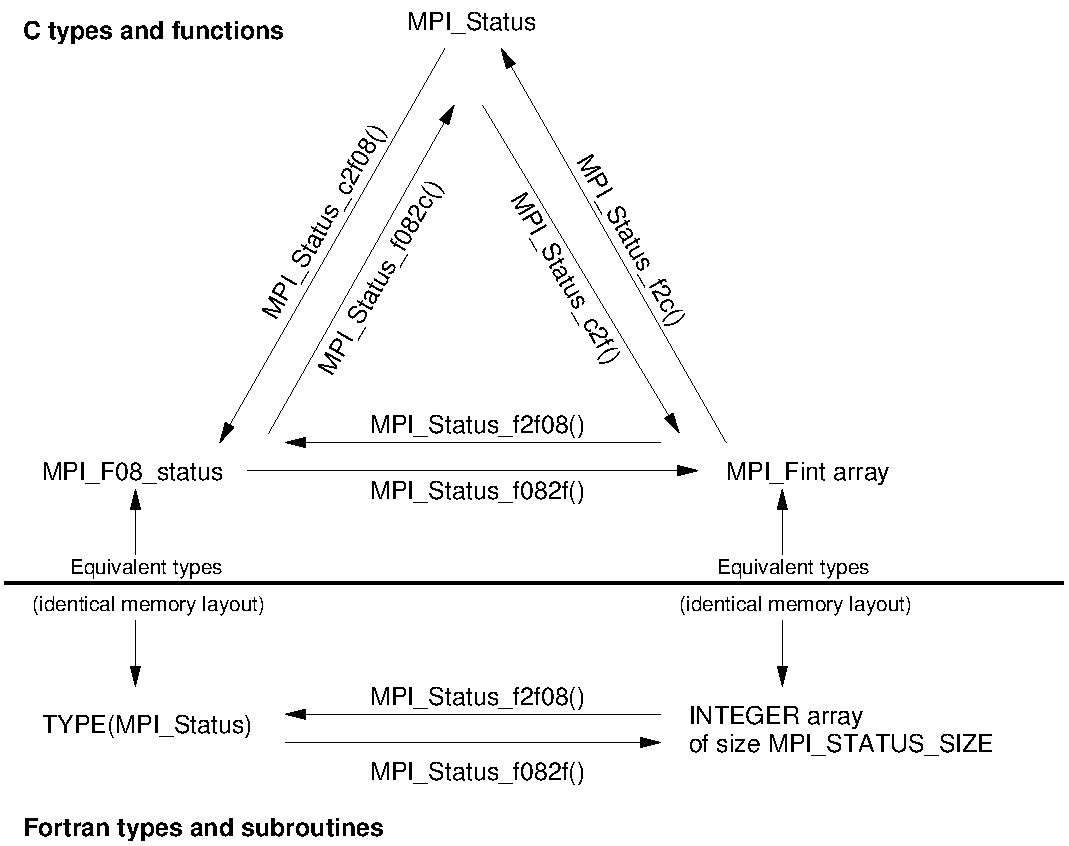
\includegraphics[width=120mm]{figures/status-conversion-triangle}}
\caption{Status conversion routines}
\label{fig:fortran:status-conversion-triangle}
\end{figure}

\cdeclindex{MPI\_Status}%
\mpiemptybindidx{MPI\_Status\_f082c}{(\gb{}const~MPI\_F08\_status~*f08\_status, MPI\_Status~*c\_status)}{int}{MPI\_STATUS\_F082C}

This C routine converts a Fortran \code{mpi\_f08} \mpiftype{TYPE(MPI\_Status)}\cdeclindex{MPI\_Status}
into a C \mpictype{MPI\_Status}.

\cdeclindex{MPI\_Status}%
\mpiemptybindidx{MPI\_Status\_c2f08}{(\gb{}const~MPI\_Status~*c\_status, MPI\_F08\_status~*f08\_status)}{int}{MPI\_STATUS\_C2F08}

This C routine converts a C \mpictype{MPI\_Status}
into a Fortran \code{mpi\_f08} \mpiftype{TYPE(MPI\_Status)}\cdeclindex{MPI\_Status}.
Two global variables of type \code{MPI\_F08\_status*},
\mpiconstmain{MPI\_F08\_STATUS\_IGNORE} and \mpiconstmain{MPI\_F08\_STATUSES\_IGNORE}
are declared in \code{mpi.h}.  They can be used to test, in C, whether
\mpiarg{f\_status} is the Fortran value of \mpiconst{MPI\_STATUS\_IGNORE}
or \mpiconst{MPI\_STATUSES\_IGNORE} defined in the \code{mpi\_f08} module.
These are global
variables, not C constant expressions and cannot be used in places
where C requires constant expressions. Their value is defined only
between the calls to \mpifunc{MPI\_INIT} and \mpifunc{MPI\_FINALIZE}
and should not be changed by user code.


Conversion between the two Fortran versions of a status can be done with:

\label{sec:conversion:status:status_f2f08}
\begin{funcdef}{MPI\_STATUS\_F2F08}{(\mbox{f\_status}, \mbox{f08\_status})}
\funcarg{\IN}{f\_status}{status object declared as array (status)}
\funcarg{\OUT}{f08\_status}{status object declared as named type (status)}
\end{funcdef}
\mpibindmain{MPI\_Status\_f2f08}{(\gb{}const~MPI\_Fint~*f\_status, MPI\_F08\_status~*f08\_status)}
\mpifnewbindmain{MPI\_Status\_f2f08}{(f\_status, f08\_status, ierror) \fargs INTEGER, INTENT(IN)\ ::\ \mbox{f\_status(MPI\_STATUS\_SIZE)}\fnarg{}TYPE(MPI\_Status), INTENT(OUT)\ ::\ \mbox{f08\_status}\fnfinalarg{}INTEGER, OPTIONAL, INTENT(OUT)\ ::\ \mbox{ierror}}
\mpifbindspecial{MPI\_STATUS\_F2F08}{(F\_STATUS, F08\_STATUS, IERROR) \fargs INTEGER :: \mbox{F\_STATUS(MPI\_STATUS\_SIZE)}, \mbox{IERROR}\fnfinalarg{}TYPE(MPI\_Status) :: \mbox{F08\_STATUS}}

This routine converts a Fortran \ftype{INTEGER}, \ftype{DIMENSION(MPI\_STATUS\_SIZE)} status array
into a Fortran \code{mpi\_f08} \mpiftype{TYPE(MPI\_Status)}\cdeclindex{MPI\_Status}.

\begin{funcdef}{MPI\_STATUS\_F082F}{(\mbox{f08\_status}, \mbox{f\_status})}
\funcarg{\IN}{f08\_status}{status object declared as named type (status)}
\funcarg{\OUT}{f\_status}{status object declared as array (status)}
\end{funcdef}
\mpibindmain{MPI\_Status\_f082f}{(\gb{}const~MPI\_F08\_status~*f08\_status, MPI\_Fint~*f\_status)}
\mpifnewbindmain{MPI\_Status\_f082f}{(f08\_status, f\_status, ierror) \fargs TYPE(MPI\_Status), INTENT(IN)\ ::\ \mbox{f08\_status}\fnarg{}INTEGER, INTENT(OUT)\ ::\ \mbox{f\_status(MPI\_STATUS\_SIZE)}\fnfinalarg{}INTEGER, OPTIONAL, INTENT(OUT)\ ::\ \mbox{ierror}}
\mpifbindspecial{MPI\_STATUS\_F082F}{(F08\_STATUS, F\_STATUS, IERROR) \fargs TYPE(MPI\_Status) :: \mbox{F08\_STATUS}\fnfinalarg{}INTEGER :: \mbox{F\_STATUS(MPI\_STATUS\_SIZE)}, \mbox{IERROR}}

This routine converts a Fortran \code{mpi\_f08} \mpiftype{TYPE(MPI\_Status)}\cdeclindex{MPI\_Status}
into a Fortran \ftype{INTEGER}, \ftype{DIMENSION(MPI\_STATUS\_SIZE)} status array.

\subsection{\texorpdfstring{\MPI/}{MPI} Opaque Objects}
\mpitermtitleindex{opaque objects}
\label{subsec:mpiopaqueobjects}

Unless said otherwise, opaque objects are ``the same'' in all languages:
they carry the same information, and have the same meaning in both
languages.  The mechanism described in the previous section can be
used to pass references to \MPI/ objects from language to language.
An object created in one language can be accessed, modified or freed
in another language.

We examine below in more detail issues that arise for each type of
\MPI/ object.

\subsubsection{Datatypes}
\mpitermtitleindex{datatypes}
\label{sec:misc-datatypes}

Datatypes encode the same information in all languages.  E.g., a
datatype accessor like \mpifunc{MPI\_TYPE\_GET\_EXTENT} will return the
same information in all languages.
If a datatype defined in
one language is used for a communication call in another language, then the
message sent will
be identical to the message that would be sent from the first language: the
same
communication buffer is accessed, and the same representation
conversion is performed, if needed.
All predefined
datatypes can be used in datatype constructors in any language. If
a datatype is committed, it can be used for
communication in any language.

The function \mpifunc{MPI\_GET\_ADDRESS} returns the same value in
all languages.  Note that we do not require that the
constant \mpiconst{MPI\_BOTTOM} have the same value in all languages (see
\sectionref{sec:misc-constants}).

\begin{example}
Absolute addresses and the conversion of datatype handles in a mixed Fortran/C program.
\Exindex{Fortran}{C/Fortran handle conversion and absolute addresses}{MPI\_Get\_address}%
\label{sec:misc-interlangcom}
% following 4 lines have been substituted:
%  INTEGER TYPE, IERR
%  INTEGER(KIND=MPI_ADDRESS_KIND) ADDR
%  CALL MPI_GET_ADDRESS(R, ADDR, IERR)
%  CALL MPI_TYPE_CREATE_STRUCT(1, 5, ADDR, MPI_REAL, TYPE, IERR)
%%HEADER
%%LANG: FORTRAN
%%FRAGMENT
%%DECL: interface
%%DECL: subroutine c_routine(val)
%%DECL: integer val
%%DECL: end subroutine c_routine
%%DECL: end interface
%%ENDHEADER
\begin{lstlisting}[language={[MPI]Fortran}]
! FORTRAN CODE
REAL :: R(5)
INTEGER :: DTYPE, IERR, AOBLEN(1), AOTYPE(1)
INTEGER(KIND=MPI_ADDRESS_KIND) :: AODISP(1)

! create an absolute datatype for array R
AOBLEN(1) = 5
CALL MPI_GET_ADDRESS(R, AODISP(1), IERR)
AOTYPE(1) = MPI_REAL
CALL MPI_TYPE_CREATE_STRUCT(1, AOBLEN, AODISP, AOTYPE, DTYPE, IERR)
CALL C_ROUTINE(DTYPE)
\end{lstlisting}

%%HEADER
%%LANG: C
%%ENDHEADER
\begin{lstlisting}[language={[MPI]C}]
/* C code */

void C_ROUTINE(MPI_Fint *ftype)
{
   int count = 5;
   int lens[2] = {1,1};
   MPI_Aint displs[2];
   MPI_Datatype types[2], newtype;

   /* create an absolute datatype for buffer that consists   */
   /*  of count, followed by R(5)                            */

   MPI_Get_address(&count, &displs[0]);
   displs[1] = 0;
   types[0] = MPI_INT;
   types[1] = MPI_Type_f2c(*ftype);
   MPI_Type_create_struct(2, lens, displs, types, &newtype);
   MPI_Type_commit(&newtype);

   MPI_Send(MPI_BOTTOM, 1, newtype, 1, 0, MPI_COMM_WORLD);
   /* the message sent contains an int count of 5, followed  */
   /* by the 5 REAL entries of the Fortran array R.          */
}
\end{lstlisting}
\end{example}

\begin{implementors}
The following implementation can be used:  \MPI/ addresses, as
returned by \mpifunc{MPI\_GET\_ADDRESS}, will have
the same value in all languages.
One obvious choice is that
\MPI/ addresses be identical to regular addresses.
The address is stored in the
datatype, when datatypes with absolute addresses are constructed.
When a send or receive operation is performed, then addresses stored in
a datatype are interpreted as displacements that are all augmented by
a base address.  This base address is (the address of) \mpiarg{buf},
or zero, if \mpiarg{buf}\mpicode{ = }\mpiconst{MPI\_BOTTOM}.  Thus, if
\mpiconst{MPI\_BOTTOM} is zero then a send or
receive call with \mpiarg{buf}\mpicode{ = }\mpiconst{MPI\_BOTTOM} is implemented
exactly as a call with a regular buffer argument:  in both cases the
base address is \mpiarg{buf}.
On the other
hand, if \mpiconst{MPI\_BOTTOM} is not zero, then the
implementation has to be slightly different.  A test is performed
to check whether \mpiarg{buf}\mpicode{ = }\mpiconst{MPI\_BOTTOM}.  If true, then
the base address is zero, otherwise it is \mpiarg{buf}.
In particular, if \mpiconst{MPI\_BOTTOM} does not have the same value in
Fortran and C,
then an additional test for \mpiarg{buf}\mpicode{ = }\mpiconst{MPI\_BOTTOM}
is needed in at least one of the languages.

It may be desirable to use a value other than zero for
\mpiconst{MPI\_BOTTOM} even in C,
so as to distinguish it from a NULL
pointer.
If \mpiconst{MPI\_BOTTOM}\ =\ c then one can still avoid the test
\mpiarg{buf}\mpicode{ = }\mpiconst{MPI\_BOTTOM}, by using the displacement from
\mpiconst{MPI\_BOTTOM}, i.e., the regular address $-$ c, as the \MPI/ address
returned by \mpifunc{MPI\_GET\_ADDRESS} and stored in absolute datatypes.
\end{implementors}


\subsubsection{Callback Functions}
\mpitermtitleindex{callback functions!language interoperability}

\MPI/ calls may associate callback functions with \MPI/
objects: error handlers are associated with communicators, files, windows, and sessions; attribute copy
and
delete functions are associated with attribute keys; reduce operations
are
associated
with operation objects, etc.  In a multilanguage
environment, a function passed in an \MPI/ call in one language may be
invoked by an \MPI/ call in another language.  \MPI/ implementations
must make sure that such invocation will use the calling convention of
the language the function is bound to.

\begin{implementors}
Callback functions need to have a language tag.  This tag is set
when the callback function is passed in by the library function (which
is presumably different for each language and language support method),
and is used to generate
the right calling sequence when the callback function is invoked.
\end{implementors}

\begin{users}
\label{advice:bindings:predefined:Fortran:users}%
If a subroutine written in one language or Fortran support method wants to
pass a callback routine including the predefined Fortran functions (e.g.,
\mpiconstfunc{MPI\_COMM\_NULL\_COPY\_FN}) to another application routine written in another language
or Fortran support method, then it must be guaranteed that both routines use the callback
interface definition that is defined for the argument when passing the callback to an \MPI/
routine (e.g., \mpifunc{MPI\_COMM\_CREATE\_KEYVAL});
see also the advice to users on page~\pageref{advice:context:predefined:Fortran:users}.
\end{users}

\subsubsection{Error Handlers}
\mpitermtitleindex{error handling!error handlers}

\begin{implementors}
Error handlers, have,
in C, a variable length argument list.
It might be useful to
provide to the handler information on the language environment where
the error occurred.
\end{implementors}

\subsubsection{Reduce Operations}
\mpitermtitleindex{reduction operations}

All predefined named and unnamed datatypes as
listed in \sectionref{coll-predefined-op} can be used in the listed
predefined operations independent of the programming language from
which the \MPI/ routine is called.

\begin{users}
Reduce operations receive as one of their arguments the datatype of the
operands.
Thus, one can define ``polymorphic'' reduce
operations that work for C and Fortran datatypes.
\end{users}

\subsection{Attributes}
\mpitermtitleindex{attribute}
\label{sec:misc-attr}


Attribute keys can be allocated in one language and freed in another.
Similarly, attribute values can be set in one language and accessed in
another.  To achieve this, attribute keys will be allocated in an integer
range that is valid all languages.  The same holds true for system-defined
attribute values (such as \mpiconst{MPI\_TAG\_UB},
\mpiconst{MPI\_WTIME\_IS\_GLOBAL}, etc.).

Attribute keys declared in one language are associated with copy and
delete functions in that language
\mpifuncindex{MPI\_TYPE\_CREATE\_KEYVAL}%
\mpifuncindex{MPI\_COMM\_CREATE\_KEYVAL}%
\mpifuncindex{MPI\_WIN\_CREATE\_KEYVAL}%
\mpifuncindex{MPI\_TYPE\_CREATE\_KEYVAL}%
\mpifuncindex{MPI\_COMM\_CREATE\_KEYVAL}%
\mpifuncindex{MPI\_WIN\_CREATE\_KEYVAL}%
(the functions provided by the \mpiskipfunc{MPI\_\XXX/\_CREATE\_KEYVAL} call).
When a
communicator is duplicated, for each attribute, the corresponding copy
function is called, using the right calling
convention for the language of that function; and similarly, for the
delete callback function.

\begin{implementors}
This requires that attributes be tagged either as
``C'' or ``Fortran''
 and that the language tag be checked in order to use
the right calling convention for the callback function.
\end{implementors}

The attribute manipulation functions described in
\sectionref{sec:caching}
defines
attributes arguments to be of type \code{void*} in C, and of type
\ftype{INTEGER}, in Fortran.  On some systems,
\ftype{INTEGER}s will have 32 bits, while
C pointers will have
64 bits.  This is a problem if communicator attributes are used to
move information from a Fortran caller to a
C callee, or
vice-versa.

\MPI/ behaves as if it stores,
internally, address sized attributes.  If Fortran \ftype{INTEGER}s
are smaller, then the (deprecated) Fortran function \mpifunc{MPI\_ATTR\_GET} will
return the least significant part of the attribute word; the (deprecated) Fortran
function \mpifunc{MPI\_ATTR\_PUT} will set the least significant part
of the attribute word, which will be sign extended to the entire word.
(These two functions may be invoked explicitly by user code, or
implicitly, by attribute copying callback functions.)

As for addresses, new functions are provided that manipulate
Fortran address sized attributes, and have the same functionality as the
old
functions in C.  These functions are described in
\sectionref{sec:caching}.
Users are encouraged to use these new functions.


\MPI/ supports two types of attributes:  address-valued (pointer) attributes,
and integer-valued attributes.  C
attribute functions put and get address-valued
attributes.  Fortran attribute functions put and get integer-valued
attributes.  When an integer-valued attribute is accessed from
C,
then
\cfunc{MPI\_\XXX/\_get\_attr}
will return the address of (a pointer to) the integer-valued
attribute, which is a pointer to
  \mpictype{MPI\_Aint} if the attribute was stored with Fortran
\mpifuncindex{MPI\_COMM\_SET\_ATTR}\mpifuncindex{MPI\_TYPE\_SET\_ATTR}\mpifuncindex{MPI\_WIN\_SET\_ATTR}%
  \mpiskipfunc{MPI\_\XXX/\_SET\_ATTR}, and a pointer to \ctype{int} if it was
  stored with the deprecated Fortran \mpifunc{MPI\_ATTR\_PUT}.  When an
address-valued attribute is accessed from
\mpifuncindex{MPI\_COMM\_GET\_ATTR}\mpifuncindex{MPI\_TYPE\_GET\_ATTR}\mpifuncindex{MPI\_WIN\_GET\_ATTR}%
Fortran, then \mpiskipfunc{MPI\_\XXX/\_GET\_ATTR}
will convert the address into an integer and
return the result of this conversion.  This conversion is lossless if new
style
attribute functions are used, and an integer of kind
\mpiconst{MPI\_ADDRESS\_KIND}
is returned.  The conversion may cause truncation if
deprecated
attribute functions are used.
In C, the deprecated routines
\mpifuncindex{MPI\_ATTR\_PUT}\mpifuncindex{MPI\_ATTR\_GET}%
  \cfunc{MPI\_Attr\_put} and \cfunc{MPI\_Attr\_get} behave identical
\mpifuncindex{MPI\_COMM\_SET\_ATTR}\mpifuncindex{MPI\_COMM\_GET\_ATTR}%
  to \cfunc{MPI\_Comm\_set\_attr} and \cfunc{MPI\_Comm\_get\_attr}.


\label{exa:misc-attr:c:pagebegin}%
\begin{example}
Setting an attribute in C and reading in C or Fortran.
\exindex{Attributes between languages}%
\Exindex[Attributes between languages, set in C]{C}{Attributes between languages!set in C}{MPI\_Comm\_set\_attr,MPI\_Comm\_get\_attr}%
\label{exa:misc-attr:c}%

A. Setting an attribute value in C
%%HEADER
%%LANG: C
%%FRAGMENT
%%DECL: int keyval1=0, keyval2=0, keyval3=0;
%%DECL: struct foo { int a; };
%%ENDHEADER
\begin{lstlisting}[language={[MPI]C}]
int set_val = 3;
struct foo set_struct;

/* Set a value that is a pointer to an int */

MPI_Comm_set_attr(MPI_COMM_WORLD, keyval1, &set_val);
/* Set a value that is a pointer to a struct */
MPI_Comm_set_attr(MPI_COMM_WORLD, keyval2, &set_struct);
/* Set an integer value */
MPI_Comm_set_attr(MPI_COMM_WORLD, keyval3, (void *) 17);
\end{lstlisting}

B. Reading the attribute value in C

%%HEADER
%%LANG: C
%%FRAGMENT
%%DECL: int keyval1=0, keyval2=0, keyval3=0;
%%ENDHEADER
\begin{lstlisting}[language={[MPI]C}]
int flag, *get_val;
struct foo *get_struct;

/* Upon successful return, get_val == &set_val
   (and therefore *get_val == 3) */
MPI_Comm_get_attr(MPI_COMM_WORLD, keyval1, &get_val, &flag);
/* Upon successful return, get_struct == &set_struct */
MPI_Comm_get_attr(MPI_COMM_WORLD, keyval2, &get_struct, &flag);
/* Upon successful return, get_val == (void*) 17 */
/*        i.e., (MPI_Aint) get_val == 17 */
MPI_Comm_get_attr(MPI_COMM_WORLD, keyval3, &get_val, &flag);
\end{lstlisting}

C. Reading the attribute value with (deprecated) Fortran \MPII/ calls

%%HEADER
%%LANG: Fortran
%%FRAGMENT
%%DECL: integer keyval1, keyval2, keyval3
%%ENDHEADER
\begin{lstlisting}[language={[MPI]Fortran}]
LOGICAL FLAG
INTEGER IERR, GET_VAL, GET_STRUCT

! Upon successful return, GET_VAL == &set_val, possibly truncated
CALL MPI_ATTR_GET(MPI_COMM_WORLD, KEYVAL1, GET_VAL, FLAG, IERR)
! Upon successful return, GET_STRUCT == &set_struct, possibly truncated
CALL MPI_ATTR_GET(MPI_COMM_WORLD, KEYVAL2, GET_STRUCT, FLAG, IERR)
! Upon successful return, GET_VAL == 17
CALL MPI_ATTR_GET(MPI_COMM_WORLD, KEYVAL3, GET_VAL, FLAG, IERR)
\end{lstlisting}

D. Reading the attribute value with Fortran \MPIII/ calls

%%HEADER
%%LANG: Fortran
%%FRAGMENT
%%DECL: integer keyval1, keyval2, keyval3
%%ENDHEADER
\begin{lstlisting}[language={[MPI]Fortran}]
LOGICAL FLAG
INTEGER IERR
INTEGER(KIND=MPI_ADDRESS_KIND) GET_VAL, GET_STRUCT

! Upon successful return, GET_VAL == &set_val
CALL MPI_COMM_GET_ATTR(MPI_COMM_WORLD, KEYVAL1, GET_VAL, FLAG, IERR)
! Upon successful return, GET_STRUCT == &set_struct
CALL MPI_COMM_GET_ATTR(MPI_COMM_WORLD, KEYVAL2, GET_STRUCT, FLAG, IERR)
! Upon successful return, GET_VAL == 17
CALL MPI_COMM_GET_ATTR(MPI_COMM_WORLD, KEYVAL3, GET_VAL, FLAG, IERR)
\end{lstlisting}
\end{example}

\begin{example}
\label{exa:misc-attr:f-old}%
Setting an attribute in Fortran and reading in C or Fortran.
\Exindex[Attributes between languages, set in Fortran]{Fortran}{Attributes between languages!set in Fortran}{MPI\_ATTR\_PUT,MPI\_ATTR\_GET,MPI\_COMM\_GET\_ATTR}%

A. Setting an attribute value with the (deprecated) Fortran \MPII/ call

%%HEADER
%%LANG: Fortran
%%FRAGMENT
%%DECL: integer keyval
%%ENDHEADER
\begin{lstlisting}[language={[MPI]Fortran}]
INTEGER IERR, VAL
VAL = 7
CALL MPI_ATTR_PUT(MPI_COMM_WORLD, KEYVAL, VAL, IERR)
\end{lstlisting}

B. Reading the attribute value in C

%%HEADER
%%LANG: C
%%FRAGMENT
%%DECL: int keyval=0;
%%ENDHEADER
\begin{lstlisting}[language={[MPI]C}]
int flag;
int *value;

/* Upon successful return, value points to internal MPI storage and
   *value == (int) 7 */
MPI_Comm_get_attr(MPI_COMM_WORLD, keyval, &value, &flag);
\end{lstlisting}

C. Reading the attribute value with (deprecated) Fortran \MPII/ calls

%%HEADER
%%LANG: Fortran
%%FRAGMENT
%%DECL: integer keyval
%%ENDHEADER
\begin{lstlisting}[language={[MPI]Fortran}]
LOGICAL FLAG
INTEGER IERR, VALUE

! Upon successful return, VALUE == 7
CALL MPI_ATTR_GET(MPI_COMM_WORLD, KEYVAL, VALUE, FLAG, IERR)
\end{lstlisting}

D. Reading the attribute value with Fortran \MPIII/ calls

%%HEADER
%%LANG: Fortran
%%FRAGMENT
%%DECL: integer keyval
%%ENDHEADER
\begin{lstlisting}[language={[MPI]Fortran}]
LOGICAL FLAG
INTEGER IERR
INTEGER(KIND=MPI_ADDRESS_KIND) VALUE

! Upon successful return, VALUE == 7 (sign extended)
CALL MPI_COMM_GET_ATTR(MPI_COMM_WORLD, KEYVAL, VALUE, FLAG, IERR)
\end{lstlisting}
\end{example}

\label{exa:misc-attr:f-new:pagebegin}

\begin{example}
\label{exa:misc-attr:f-new}%
Setting an attribute in Fortran and reading in C or Fortran.
\Exindex[Attributes between languages, set in Fortran]{Fortran}{Attributes between languages!set in Fortran}{MPI\_COMM\_SET\_ATTR,MPI\_ATTR\_GET,MPI\_COMM\_GET\_ATTR}%

A. Setting an attribute value via a Fortran \MPIII/ call

%%HEADER
%%LANG: Fortran
%%FRAGMENT
%%DECL: integer keyval1, keyval2
%%ENDHEADER
\begin{lstlisting}[language={[MPI]Fortran}]
INTEGER IERR
INTEGER(KIND=MPI_ADDRESS_KIND) VALUE1
INTEGER(KIND=MPI_ADDRESS_KIND) VALUE2
VALUE1 = 42
VALUE2 = INT(2, KIND=MPI_ADDRESS_KIND) ** 40

CALL MPI_COMM_SET_ATTR(MPI_COMM_WORLD, KEYVAL1, VALUE1, IERR)
CALL MPI_COMM_SET_ATTR(MPI_COMM_WORLD, KEYVAL2, VALUE2, IERR)
\end{lstlisting}

B. Reading the attribute value in C

%%HEADER
%%LANG: C
%%FRAGMENT
%%DECL: int keyval1=0, keyval2=0;
%%ENDHEADER
\begin{lstlisting}[language={[MPI]C}]
int flag;
MPI_Aint *value1, *value2;

/* Upon successful return, value1 points to internal MPI storage and
   *value1 == 42 */
MPI_Comm_get_attr(MPI_COMM_WORLD, keyval1, &value1, &flag);
/* Upon successful return, value2 points to internal MPI storage and
   *value2 == 2^40 */
MPI_Comm_get_attr(MPI_COMM_WORLD, keyval2, &value2, &flag);
\end{lstlisting}

C. Reading the attribute value with (deprecated) Fortran \MPII/ calls

%%HEADER
%%LANG: Fortran
%%FRAGMENT
%%DECL: integer keyval1, keyval2
%%ENDHEADER
\begin{lstlisting}[language={[MPI]Fortran}]
LOGICAL FLAG
INTEGER IERR, VALUE1, VALUE2

! Upon successful return, VALUE1 == 42
CALL MPI_ATTR_GET(MPI_COMM_WORLD, KEYVAL1, VALUE1, FLAG, IERR)
! Upon successful return, VALUE2 == 2^40, or 0 if truncation
! needed (i.e., the least significant part of the attribute word)
CALL MPI_ATTR_GET(MPI_COMM_WORLD, KEYVAL2, VALUE2, FLAG, IERR)
\end{lstlisting}

D. Reading the attribute value with Fortran \MPIII/ calls

%%HEADER
%%LANG: Fortran
%%FRAGMENT
%%DECL: integer keyval1, keyval2
%%ENDHEADER
\begin{lstlisting}[language={[MPI]Fortran}]
LOGICAL FLAG
INTEGER IERR
INTEGER(KIND=MPI_ADDRESS_KIND) VALUE1, VALUE2

! Upon successful return, VALUE1 == 42
CALL MPI_COMM_GET_ATTR(MPI_COMM_WORLD, KEYVAL1, VALUE1, FLAG, IERR)
! Upon successful return, VALUE2 == 2^40
CALL MPI_COMM_GET_ATTR(MPI_COMM_WORLD, KEYVAL2, VALUE2, FLAG, IERR)
\end{lstlisting}
\end{example}


The predefined \MPI/ attributes can be integer valued or address-valued.
Predefined integer valued attributes, such as \mpiconst{MPI\_TAG\_UB},
behave as if they
were put by a call to the
  deprecated Fortran routine \mpifunc{MPI\_ATTR\_PUT},
i.e.,
in Fortran,
\mpifunc{MPI\_COMM\_GET\_ATTR}\code{(MPI\_COMM\_WORLD, MPI\_TAG\_UB, val, flag, ierr)}
will return in \mpiarg{val}
the upper bound for tag value; in C,
\mpifuncindex{MPI\_COMM\_GET\_ATTR}%
\cfunc{MPI\_Comm\_get\_attr(MPI\_COMM\_WORLD, MPI\_TAG\_UB, \&p, \&flag)}
will return in \mpiarg{p}
a pointer to an int containing the upper bound for tag value.

Address-valued predefined attributes, such as \mpiconst{MPI\_WIN\_BASE}
behave as if
they were put by a C call,
i.e.,
in  Fortran,
\mpifunc{MPI\_WIN\_GET\_ATTR}\code{(win, MPI\_WIN\_BASE, val, flag, ierror)}
will return in \mpiarg{val} the base address of the window,
converted to an integer.  In C,
\mpifuncindex{MPI\_WIN\_GET\_ATTR}%
\cfunc{MPI\_Win\_get\_attr(win, MPI\_WIN\_BASE, \&p, \&flag)}
will return in \mpiarg{p}
a pointer to the window base, cast to \code{(void~*)}.

\begin{rationale}
The design is consistent with the behavior
specified
for predefined
attributes, and ensures that no information is lost when attributes are
passed from language to language.
Because the language interoperability for
  predefined attributes was defined based on \mpifunc{MPI\_ATTR\_PUT},
  this definition is kept for compatibility reasons although the
  routine itself is now deprecated.
\end{rationale}

\begin{implementors}
  Implementations should tag attributes either as
  (1)
    address attributes, (2) as
    \code{INTEGER(KIND=MPI\_ADDRESS\_KIND)} attributes or (3) as
    \code{INTEGER} attributes, according to whether they were set in
    (1) C (with \cfunc{MPI\_Attr\_put} or
\mpifuncindex{MPI\_COMM\_SET\_ATTR}\mpifuncindex{MPI\_TYPE\_SET\_ATTR}\mpifuncindex{MPI\_WIN\_SET\_ATTR}%
    \cfunc{MPI\_\XXX/\_set\_attr}), (2) in Fortran with
    \ffunc{MPI\_\XXX/\_SET\_ATTR} or (3) with the deprecated Fortran
\mpifuncindex{MPI\_ATTR\_PUT}
    routine \ffunc{MPI\_ATTR\_PUT}.
    Thus, the right choice can be made when the attribute is retrieved.
\end{implementors}

\subsection{Extra-State}
\mpitermtitleindex{extra-state}

Extra-state should not be modified by the copy or delete callback
functions.  (This is obvious from the C binding, but not obvious from the
Fortran binding).  However, these functions may update state that is
indirectly accessed via extra-state.  E.g., in C, extra-state can be a
pointer to a data structure that is modified by the copy or callback
functions; in Fortran, extra-state can be an index into an entry in a
\code{COMMON} array that is modified by the copy or callback functions.  In a
multithreaded environment, users should be aware that distinct threads may
invoke the same callback function concurrently: if this function modifies
state associated with extra-state, then mutual exclusion code must be used
to protect updates and accesses to the shared state.


\subsection{Constants}
\mpitermtitleindex{constants}
\label{sec:misc-constants}

\MPI/ constants have the same value in all languages,
unless specified otherwise.
This does not apply to constant handles (\type{MPI\_INT},
\mpiconst{MPI\_COMM\_WORLD}, \mpiconst{MPI\_ERRORS\_RETURN},
\mpiconst{MPI\_SUM}, etc.)
These handles need to be converted, as explained in
Section~\ref{sec:misc-handleconvert}.
Constants that specify maximum lengths of strings (see
Section~\ref{subsec:annexa-const} for a listing) have a value one less
in Fortran than C since in
C the length includes the null
terminating character. Thus, these constants represent the amount of
space that must be allocated to hold the largest possible such
string, rather than the maximum number of printable characters the
string could contain.

\begin{users}
This definition means that it is safe in C
to allocate a buffer to receive
a string using a declaration like
%%HEADER
%%LANG: C
%%FRAGMENT
%%TAIL: if (name[0]) exit(1);
%%ENDHEADER
\begin{lstlisting}[language={[MPI]C}]
char name [MPI_MAX_OBJECT_NAME];
\end{lstlisting}
\end{users}

Also constant ``addresses,'' i.e., special values for reference
arguments that are not handles, such as  \mpiconst{MPI\_BOTTOM} or
\mpiconst{MPI\_STATUS\_IGNORE} may
have different values in different languages.


\begin{rationale}
The current \MPI/ standard specifies that \mpiconst{MPI\_BOTTOM} can be
used in initialization expressions in C, but not in Fortran.  Since
Fortran does not normally support call by value, then
\mpiconst{MPI\_BOTTOM} in Fortran must be the name of a predefined
static variable, e.g., a variable in an \MPI/ declared \ftype{COMMON}
block. On the other hand, in C, it is natural to take
\mpiconst{MPI\_BOTTOM}\ =\ 0 (Caveat: Defining \mpiconst{MPI\_BOTTOM}\ =\ 0
implies that \code{NULL} pointer cannot be distinguished from
\mpiconst{MPI\_BOTTOM}; it may be that \mpiconst{MPI\_BOTTOM}\ =\ 1 is better.
See the advice to implementors in the \nameref{sec:misc-datatypes} subsection in
Section~\ref{subsec:mpiopaqueobjects})
Requiring that the Fortran and C values be the same will complicate
the initialization process.
\end{rationale}

\subsection{Interlanguage Communication}
\mpitermtitleindex{interlanguage communication}
\label{subsec:interlanguage-communication}
The type matching rules for communication in \MPI/ are not changed:
the datatype specification for each item sent should match,
in type signature, the datatype specification used to receive this item
(unless one of the types is \type{MPI\_PACKED}).
Also, the
type of a message item should match the type declaration for the
corresponding communication buffer location, unless the type is
\type{MPI\_BYTE} or \type{MPI\_PACKED}.  Interlanguage
communication is allowed if it complies with these rules.

\begin{example}
\exindex{Interlanguage communication}%
\Exindex{Fortran}{Interlanguage communication}{MPI\_Type\_create\_struct,MPI\_Get\_address}%
In the example below, a Fortran array is sent from Fortran and received in
C.

% following 4 lines have been substituted:
%  INTEGER TYPE, IERR, MYRANK
%  INTEGER(KIND=MPI_ADDRESS_KIND) ADDR
%  CALL MPI_GET_ADDRESS(R, ADDR, IERR)
%  CALL MPI_TYPE_CREATE_STRUCT(1, 5, ADDR, MPI_REAL, TYPE, IERR)
%%HEADER
%%LANG: FORTRAN08
%%ALLOWMISMATCH
%%ENDHEADER
\begin{lstlisting}[language={[MPI08]Fortran}]
! FORTRAN CODE
SUBROUTINE MYEXAMPLE()
USE mpi_f08
REAL :: R(5)
INTEGER :: IERR, MYRANK, AOBLEN(1)
TYPE(MPI_Datatype) :: DTYPE, AOTYPE(1)
INTEGER(KIND=MPI_ADDRESS_KIND) :: AODISP(1)

! create an absolute datatype for array R
AOBLEN(1) = 5
CALL MPI_GET_ADDRESS(R, AODISP(1), IERR)
AOTYPE(1) = MPI_REAL
CALL MPI_TYPE_CREATE_STRUCT(1, AOBLEN, AODISP, AOTYPE, DTYPE, IERR)
CALL MPI_TYPE_COMMIT(DTYPE, IERR)

CALL MPI_COMM_RANK(MPI_COMM_WORLD, MYRANK, IERR)
IF (MYRANK .EQ. 0) THEN
   CALL MPI_SEND(MPI_BOTTOM, 1, DTYPE, 1, 0, MPI_COMM_WORLD, IERR)
ELSE
   CALL C_ROUTINE(DTYPE%MPI_VAL)
END IF
END SUBROUTINE
\end{lstlisting}

%%HEADER
%%LANG: C
%%ENDHEADER
\begin{lstlisting}[language={[MPI]C}]
/* C code */

void C_ROUTINE(MPI_Fint *fhandle)
{
   MPI_Datatype type;
   MPI_Status status;

   type = MPI_Type_f2c(*fhandle);

   MPI_Recv(MPI_BOTTOM, 1, type, 0, 0, MPI_COMM_WORLD, &status);
}
\end{lstlisting}
\end{example}

\MPI/ implementors may weaken these type matching rules, and allow
messages to be sent with Fortran types and received with C types, and
vice versa, when those types match.  I.e., if the Fortran type
\ftype{INTEGER} is identical to the C type
\ctype{int}, then an \MPI/ implementation may allow data to be sent
with datatype \type{MPI\_INTEGER} and be received with datatype
\type{MPI\_INT}.  However, such code is not portable.

